\documentclass[11pt, twoside]{uwthesis}
% ***********************************************************
% ******************* PHYSICS HEADER ************************
% ***********************************************************
% Version 2
%\documentclass[11pt]{article} 
\usepackage{amsmath} % AMS Math Package
\usepackage{amsthm} % Theorem Formatting
\usepackage{amssymb}	% Math symbols such as \mathbb
\usepackage{graphicx} % Allows for eps images
\usepackage{multicol} % Allows for multiple columns
%\usepackage[dvips,letterpaper,margin=0.75in,bottom=0.5in]{geometry}
 % Sets margins and page size
%\pagestyle{empty} % Removes page numbers
%\makeatletter % Need for anything that contains an @ command 
%\renewcommand{\maketitle} % Redefine maketitle to conserve space
%{ \begingroup \vskip 10pt \begin{center} \large {\bf \@title}
	%\vskip 10pt \large \@author \hskip 20pt \@date \end{center}
  %\vskip 10pt \endgroup \setcounter{footnote}{0} }
%\makeatother % End of region containing @ commands
\renewcommand{\labelenumi}{(\alph{enumi})} % Use letters for enumerate
% \DeclareMathOperator{\Sample}{Sample}
\let\vaccent=\v % rename builtin command \v{} to \vaccent{}
\renewcommand{\v}[1]{\ensuremath{\mathbf{#1}}} % for vectors
\newcommand{\gv}[1]{\ensuremath{\mbox{\boldmath$ #1 $}}} 
% for vectors of Greek letters
\newcommand{\uv}[1]{\ensuremath{\mathbf{\hat{#1}}}} % for unit vector
\newcommand{\abs}[1]{\left| #1 \right|} % for absolute value
\newcommand{\avg}[1]{\left< #1 \right>} % for average
\let\underdot=\d % rename builtin command \d{} to \underdot{}
\renewcommand{\d}[2]{\frac{d #1}{d #2}} % for derivatives
\newcommand{\dd}[2]{\frac{d^2 #1}{d #2^2}} % for double derivatives
\newcommand{\pd}[2]{\frac{\partial #1}{\partial #2}} 
% for partial derivatives
\newcommand{\pdd}[2]{\frac{\partial^2 #1}{\partial #2^2}} 
% for double partial derivatives
\newcommand{\pdc}[3]{\left( \frac{\partial #1}{\partial #2}
 \right)_{#3}} % for thermodynamic partial derivatives
\newcommand{\ket}[1]{\left| #1 \right>} % for Dirac bras
\newcommand{\bra}[1]{\left< #1 \right|} % for Dirac kets
\newcommand{\braket}[2]{\left< #1 \vphantom{#2} \right|
 \left. #2 \vphantom{#1} \right>} % for Dirac brackets
\newcommand{\matrixel}[3]{\left< #1 \vphantom{#2#3} \right|
 #2 \left| #3 \vphantom{#1#2} \right>} % for Dirac matrix elements
\newcommand{\grad}[1]{\gv{\nabla} #1} % for gradient
\let\divsymb=\div % rename builtin command \div to \divsymb
\renewcommand{\div}[1]{\gv{\nabla} \cdot #1} % for divergence
\newcommand{\curl}[1]{\gv{\nabla} \times #1} % for curl
\let\baraccent=\= % rename builtin command \= to \baraccent
\renewcommand{\=}[1]{\stackrel{#1}{=}} % for putting numbers above =
\newtheorem{prop}{Proposition}
\newtheorem{thm}{Theorem}[section]
\newtheorem{lem}[thm]{Lemma}
\theoremstyle{definition}
\newtheorem{dfn}{Definition}
\theoremstyle{remark}
\newtheorem*{rmk}{Remark}

% ***********************************************************
% ********************** END HEADER *************************
% ***********************************************************

\usepackage{tabularx}
\usepackage{graphicx}
\usepackage{alltt}
\usepackage{rotating}
\usepackage{amsmath}
\usepackage[toc,page]{appendix}
\usepackage{float}
\usepackage{verbatim}
\usepackage{hyperref}


\DeclareMathOperator{\sech}{sech}
\begin{document}

\newcommand{\ion}{$^{+}$}
\newcommand{\degree}{$^{\circ}$}
\newcommand{\baseven}{$^{137}$Ba$^{+}$}
\newcommand{\ba}{$^{138}$Ba$^{+}$}
\newcommand{\curdir}{theory}

\prelimpages

\Title{Mixed Species Ion Chains for Scalable Quantum Computation}
\Author{John Albert Wright}
\Year{2015}
\Program{Department of Physics}

\Chair{Boris Blinov}{Associate Professor}{Department of Physics}
\Signature{Subhadeep Gupta}
\Signature{Xiaodong Xu}

\titlepage

\newpage
\copyrightpage

\abstract{
Mixed species chains of barium and ytterbium ions are investigated as a tool for building scalable quantum computation devices.  Ytterbium ions provide a stable, environmentally-insensitive qubit that is easily initialized and manipulated, while barium ions are easily entangled with photons that can allow quantum information to be transmitted between systems in modular quantum computation units.  Barium and ytterbium are trapped together in a linear chain in a linear rf trap and their normal mode structure and the thermal occupation numbers of these modes are measured with a narrow band laser addressing an electric quadrupole transition in barium ions. Before these measurements, barium ions are directly cooled using Doppler cooling, while the ytterbium ions are sympathetically cooled by the barium.  For radial modes strongly coupled to ytterbium ions the average thermal occupation numbers vary between 400 and 12,000 depending on ion species configuration and trap parameters.  Ion chain temperatures are also measured using a technique based on ion species reordering.  Surface traps with many dc electrodes provide the ability to controllably reorder the chain to optimize normal mode cooling, and initial work towards realizing this capability are discussed.  Quantum information can be transferred between ions in a linear chain using an optical system that is well coupled to the motional degrees of freedom of the chain.  For this reason, a 532~nm Raman system is developed and its expected performance is evaluated.

}

\tableofcontents
\listoffigures
\listoftables

\newpage
\begin{center}
{\bf\Large ABBREVIATIONS}
\end{center}
\begin{description}
	\item[ADC] Analog to Digital Converter.  Converts analog voltage or current signals to the digital representation of a corresponding number in Volts or Amperes.

	\item[AOM] Acousto-Optic Modulator.  Device to diffract an incoming laser beam against a rf standing wave.  Allows the frequency and power of a diffracted beam to be quickly controlled by changing RF parameters.

	\item[CW] Continuous Wave.  Mode of laser operation with constant light emission.  Often used to distinguish from pulsed or mode-locked operation, where the laser outputs light in discrete pulses.

	\item[DAC] Digital to Analog Converter.  Converts a digital representation of a number to a corresponding analog signal of that many Volts or Amperes.

	\item[DC] Direct Current.  Current flowing in a constant direction.  Often used to refer to signals with no time variation.

	\item[DDS] Direct Digital Synthesizer.  Frequency synthesizer with digital control interface. 

	\item[DPAOM] Double Passed Acousto-Optic Modulator.  Optical system that diffracts light twice off an AOM to increase optical isolation and minimize pointing shifts due to changing the rf frequency applied to the AOM.

	\item[DSUB] D-subminiature.  A common type of electrical connector often used for serial connections.

	\item[ECDL] External Cavity Diode Laser.  Laser made by externally frequency selecting and feeding back light into a laser diode.

	\item[EMCCD]  Electron Multiplying Charge Coupled Device. Charge coupled device with an electron multiplying readout channel with controllable gain.

	\item[EOM] Electro-Optic Modulator.  Device to modulate a laser beam with an electric control field.  Allows modulation of the frequency, power, or phase of the beam.

	\item[FPGA] Field Programmable Gate Array.  Integrated circuit with programmable interconnects between logical gates enabling rapid development of logic circuits.

	\item[HWP] Half Wave Plate. Delays light polarized along one direction by half a wavelength while not affecting the orthogonal direction of polarization.  Often used to rotate the polarization of light by a desired angle.

	\item[PBS] Polarizing Beam Splitter.  Reflects light polarized along one direction while transmitting the orthogonal direction of polarization.

	\item[PCB] Printed Circuit Board.  Insulating board with small printed conducting traces on its surface.  Often printed to implement complicated circuits without large amounts of tedious wiring.

	\item[PID Controller] Proportional, Integral, Differential Controller.  Feedback controller with three feedback terms proportional to the error signal, its integral, and its derivative.

	\item[PMT] Photomultiplier Tube.  Single photon detection device based on photoelectron amplification.

	\item[QWP] Quarter Wave Plate. Delays light polarized along one direction by a quarter of a wavelength while not affecting the orthogonal direction of polarization.  Often used to elliptically or circularly polarize light.

	\item[RF] Radio Frequency.  Frequencies between a few kHz and $\approx$ 1000~GHz.

	\item[SRAM] Static Random-Access Memory.  Digital, computer memory that is stable so long as power is provided to it.

	\item[TTL] Transistor-Transistor Logic.  Digital signaling standard using voltages between 0 and 0.8~V for ``0'' and 2.2 to 5~V for ``1''.

	\item[UHV] Ultra-High Vacuum.  Pressures below 10$^{-9}$~torr.  Usually only achievable with all metal seals and careful chamber preparation.	

	\item[UDP] User Datagram Protocol.  Protocol for sending information over an Internet Protocol network.  
\end{description}



\acknowledgments{
I would like to thank my parents, Juli and William Wright, and my stepmother, Ellen Fox, for working hard to raise me well and provide me with all the opportunities I could hope for.  I also have to thank my wonderful wife, Allison Wootan.  We have been a huge part of each other's lives for almost a decade now, and I can't imagine being here without her.  Without the love and support of these people I certainly would not have made it to where I am today.

I would also like to thank Boris Blinov for his support since the first day I arrived at the University of Washington.  He's given me the opportunity to take apart everything in our lab, and I've even managed to put most of it back together.  I can't imagine working in any other kind of lab, and I've greatly enjoyed it and learned so much from him.

I've been fortunate to work with a great team of graduate students and postdoctoral researchers.  In particular, I learned a huge fraction of what I know about ion trapping by talking with fellow graduate students Thomas Noel and Matt Hoffman.  It's been great working closely with Tomasz Sakrejda these past few years and seeing Carolyn Auchter, Spencer Williams, and CK Chou around the lab.  I've also enjoyed working with our postdocs Richard Graham and Zichao Zhou.  There have also been many undergraduates who have helped build so much of the infrastructure I use everyday including Matthew Bohman, Wen Lin Tan, Sarah Innes-Gold, Sean Nelson, and many others.

}

\textpages

\part{Quantum Computation in Ion Traps}

\chapter{Quantum Computation}
\renewcommand{\curdir}{qcomp}
\label{sec:qcomp}

\graphicspath{ {\curdir/Graphics/}  }

Quantum computation is a method for performing calculations on data that utilizes additional properties of quantum mechanics that classical computation does not.  Quantum algorithms running on capable systems will be able to perform some calculations in exponentially less time than classical computers will ever be able to.  To realize these speed increases, we need to engineer unprecedented control over thousands of coupled quantum systems.  There are a number of physical systems that have a sufficient degree of isolation from environmental noise that it is possible to consider implementing a quantum computer using them.  These systems include superconducting junctions \cite{Devoret:13}, quantum dots \cite{Kloeffell:13}, trapped neutral atoms \cite{Saffman:10}, and trapped ions.

\section{Motivating Quantum Computing}
In order to quantify the possible speed increase that quantum computers represent, it is useful to refer to the idea of complexity classes in computer science.  Complexity classes are groups of problems that share a similar dependence between the input size of a problem and the time and memory required to solve it using a given computational system.  In Figure~\ref{fig:bqp}, PSPACE, or ``polynomial space'', is the class of problems that can be solved using an amount of memory that is polynomial in the size of the problem on a classical computer.  The size of the problem in this context refers to the size required to represent the inputs of the problem in computer memory.  For example, if the input is a single number, $N$, it can be represented in memory space proportional to $\log{N}$.  For problems that require a large series of numbers as input, the logarithm of each number is approximately the same size and the problem size is often written as the number of input numbers ignoring the approximately constant multiplicative factor.  The ``nondeterministic polynomial'', or NP, complexity class in Figure~\ref{fig:bqp} is the class of problems that can be solved in an amount of computational time that is a polynomial function of the size of the input on a nondeterministic computer.  A nondeterministic computer can take multiple computational paths at every branching point in a program and determine at the end of the computation which path led to a solution.  This class of problems also has the characteristic that a possible solution can be verified in polynomial time on a classical computer.  One of the most important open questions in computer science is whether these problems that can be verified in polynomial time can also be solved in polynomial time on a classical computer, and therefore are also a member of the complexity class P, ``polynomial''.  It is generally believed that these complexity classes are not equal, that is $P \ne NP$, and therefore classical algorithms to efficiently solve NP problems will never be found.  Instead we will have to use algorithms that scale poorly with the size of the problem, and can become difficult to solve even for small scale problems.

\begin{figure}
	\centering
	
\includegraphics[width=0.4\linewidth] {BQP_complexity_class_diagram}
	\caption[Relationship of BQP complexity class to P, NP, and PSPACE]{The currently believed relationship between the BQP complexity class and other classical computing complexity classes.  BQP includes some problems from NP, as well as some problems from PSPACE outside of NP.  See text for a description of these complexity classes.}
	\label{fig:bqp}
\end{figure}

Quantum algorithms are analyzed as probabilistic algorithms that take into account the probability of the algorithm producing the wrong solution.  The computational class of problems that are easily solved using a quantum computer is named ``bounded error quantum polynomial time'', or BQP.  It is the class of problems solvable in polynomial time on a quantum computer with a probability of failure that is less than $\frac{1}{3}$.  We can see from Figure~\ref{fig:bqp} that quantum computers should be able to efficiently solve some problems that will probably never be efficiently solved classically, including some problems in NP and some problems in PSPACE that are outside of NP.

The most famous quantum algorithm is known as Shor's algorithm.  It is an algorithm for solving the discrete logarithm problem.  The inputs to the problem are two elements, $a$ and $b$, of some finite group, $G$, and the desired output is an exponent, $n$, such that $a^n = b$.  The trivial algorithm is to continuously exponentiate $a$ to higher and higher powers, which takes time proportional to the number of elements of $G$.  Since the input to the problem is two elements of G, the input size of the problem is proportional to $\log \left| G \right|$ and the na\"{\i}ve algorithm takes time proportional to $\left| G \right|$ and exponential in the input size.  Shor's algorithm provides a solution to the discrete logarithm problem that requires only time linear in the size of the input.  

Practically speaking, this problem has applications in cryptography for which groups with size $2^{256}$ or larger are often chosen. Solving this problem is the difficult task that keeps public key cryptographically secured information safe, and it is generally suspected that for sufficiently large groups it will never be solved on classical hardware.  A functional quantum computer of sufficient size could use Shor's algorithm to break all known public key cryptography techniques using a very small amount of computational time. These encryption techniques fall into two groups, those based on factoring large integers and those based on solving for roots of elliptic curves in finite fields.  Both of these problems are easy to solve in one direction, but classically very costly to solve in the opposite direction unless you know a secret piece of information.  Someone desiring to encrypt something can easily compute the result of these calculations for some given parameters, but unless you know the information used to calculate those parameters decrypting the result of the calculation is very difficult.  Both of these known public-key cryptography problems are extremely susceptible to quantum computing, because the secret information can be quickly determined from the calculation parameters.

There are also many other interested quantum algorithms.  Grover's algorithm allows a computer to find a desired item in an unordered list of $N$ items in time proportional to $\sqrt{N}$.  There are also algorithms that allow us to determine the characteristics of quantum black box devices very quickly including the Deutsch-Jozsa algorithm and Simon's algorithm.  There is still ongoing research into finding new computer science problems where quantum computers can outperform classical.

From a physicist's point of view, perhaps the larger motivation for building a quantum computer is the ability to simulate complicated quantum systems.  Trapped ion based quantum computers are beginning to approach being able to find results for physical problems that are very difficult for classical computers to solve.  In particular, frustrated magnetic systems can already be simulated using trapped ions \cite{Islam:13}, but these systems are very difficult to solve classically even for only dozens of particles.  Optical lattices of neutral atoms are also already being used to probe condensed matter states such as Mott insulators and antiferromagnetic states \cite{Bakr:09}.  Simulating full Hamiltonians of complicated systems may remain infeasible on classical computers for decades still, while because of their favorable scaling, quantum computers will be trivially able to do so.

\section{The DiVincenzo Criteria}
\label{sec:divincenzo}

Although there are many systems under investigation as potential quantum computing technologies, I am only going to seriously discuss the possibilities of trapped ion quantum computers.  In order to guide our discussion of how trapped ions represent a possible technology for implementing quantum computation, I will follow the venerable DiVincenzo criteria \cite{DiVincenzo:00}.  These five criteria were proposed by David DiVincenzo in 2000, and describe the basic requirements for a feasible quantum computing architecture.  They place limits on both the physical system chosen to represent quantum information and the technologies that isolate and interact with it.

The operational units of a quantum computer are usually referred to as qubits (short for quantum bits).  Qubits have two possible values $\ket{0}$ and $\ket{1}$ just like classical bits have two possible values 0 and 1, but they can also represent any superposition of those two values.  Two energy states in the ion are chosen to represent these two values.   The populations and coherences of these energy levels are manipulated by applying external fields.  Additionally, quantum computers can work with quantum entangled states of qubits, which is a necessary capability for the additional computational power of quantum computers.

\subsubsection{1. A scalable physical system with well characterized qubits}

The first criteria is unfortunately the one that is most difficult to realize with a trapped ion system.  The qubits themselves, represented by long-lived internal energy states of the ions, are certainly well characterized.  However, the physical system required to trap the ions and generate entanglement between them has proven difficult to scale to large numbers of ions.  Current state of the art systems can simultaneously entangle 14 qubits \cite{Monz:11}, which is already technically very challenging and still of limited use computationally.  The focus of the rest of this thesis will be on one proposal for scaling ion trap systems up to useful number of qubits.

\subsubsection{2. The ability to initialize the state of the qubits to a simple fiducial state, such as $\ket{000...}$} 

This ability is easily realized in trapped ions by tuning the polarization or frequency of a group of lasers to drive transitions from all but one accessible long-lived state, a technique called optical pumping.  The exact details depend on the species being trapped, but are usually very straightforward.  A possible procedure for an ion with a J = 1/2 excited and ground state is outlined in Figure~\ref{fig:optical-pumping}.  

Once these transitions are addressed the population will be pumped to the non-addressed long-lived state by decay from the excited states.  From this optically pumped state the qubit can be transferred to whatever state represents $\ket{0}$ in the proposed computation scheme.  In practice, only a few lasers are often necessary to realize this procedure and the desired state can be initialized with fidelities easily greater than 99\%.

\begin{figure}
	\centering
	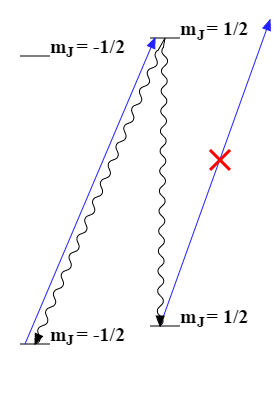
\includegraphics[width=0.35\textwidth]{optical-pumping}
	\caption[Diagram of optical pumping procedure]{Diagram of polarization optical pumping procedure.  Transitions with $\Delta m_J = 1$ are selected by applying $\sigma^+$ polarized light along the angular momentum quantization axis.  Population is pumped to the $m_J = +1/2$ level of the ground state because there are no allowed transition from that state but population can decay there after a transition from the other $m_J$ state.}
	\label{fig:optical-pumping}
\end{figure}

\subsubsection{3. Long relevant decoherence times, much longer than the gate operation time}

Once again the exact details of the implementation depend on the chosen atomic species and isotope, but there are usually several possible long lived states in a given species that could serve as qubits.  In particular, in species with odd nuclear spin there are first order magnetic field insensitive ground state levels with coherence times easily reaching several seconds \cite{Olmschenk:07,Mount:13}.  There are even energy levels separated by optical transition frequencies that have similar decoherence times.  These time scales compare very favorably with gate operation times between 1~$\mu$s and 10~$\mu$s.

\subsubsection{4. A universal set of quantum gates}

A universal set of gates refers to a set of operations that can be performed on the qubits in order to approximate any unitary operator.  In practice, the necessary set can be relatively small and involve only a few single qubit rotations and an entangling operation between qubits.  These kinds of operations are easily accomplished using external electric and magnetic fields with rf and optical frequencies.  The rotations can be accomplished with near-resonant radiation at the qubit energy. The Coulomb interaction between trapped ions provides a strong coupling between their motional energy states that can be used to perform entangling operations.  Fidelities for these operations can be very high, and gate times can be very short \cite{Mount:13}.

\subsubsection{5. A qubit-specific measurement capability}

Ions that can be trapped usually have a strong, cycling optical transition that can scatter millions of photons per second.  By manipulating the internal state of the ions to allow or disallow such a transition, the ions' state can be read out by merely collecting fluorescence.  The state can be determined by collecting fluorescence for tens of milliseconds and applying a simple threshold to separate background fluorescence from fluorescence from the ion (see Figure~\ref{fig:statedetection}).  Read out times as short as 10.5~$\mu$s with 99\% fidelity have been demonstrated \cite{Noek:13}.  This internal state manipulation is often as simple as transferring the ion to a state outside of the decay channels of the driven transition.

\begin{figure}
	\centering
	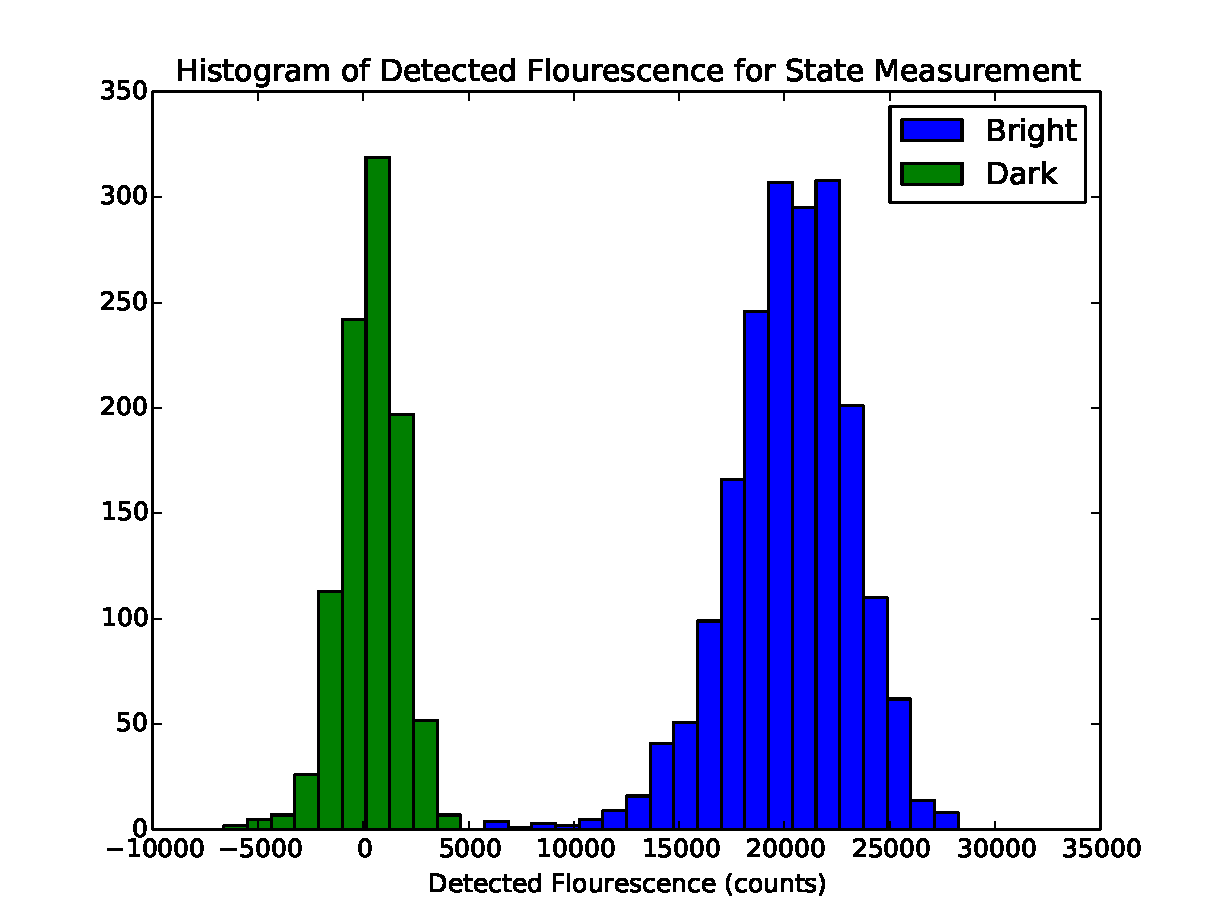
\includegraphics[width=0.6\textwidth]{StateMeasurement}
	\caption[Histogram of collected ion fluoresence for state detection]{Histogram of ion fluorescence detected with an EMCCD in 0.1~s for state detection.  A constant background has been subtracted.  ``Bright'' and ``dark'' states corresponding to the ion being in or out of the cooling cycle can be distinguished with high probability.} 
	\label{fig:statedetection}
\end{figure}

\section{Qubits and Operators}
Initialization and readout of trapped ion quantum systems requires analysis of the atomic structure of the particular choice of species.  Specific lasers and procedures are required for different ions, but only resonant transitions and fluorescence collection are required.  The necessary techniques for our ions will be discussed in Chapter~\ref{sec:ioncool}.  Quantum gates to be performed between out initialization and readout can also be engineered, but we will need to analyze the effects of nonresonant lasers and ion motional modes.  To realize a universal quantum computer we must be able to perform each gate in a universal set of quantum gates.  There are many possible choices for such a set, but I will consider the Hadamard (H), the $\frac{\pi}{8}$ (T), and controlled-not (CNOT) gates.  These gates can be represented as the unitary matrices
\begin{equation}
	U_H = \frac{1}{\sqrt{2}} \left( \begin{array}{cc} 
		1 & 1 \\ 1 & -1 
	\end{array} \right) \quad
	U_T = \left( \begin{array}{cc} 
		1 & 0 \\ 0 & e^{i \frac{\pi}{4}}
	\end{array} \right) \quad
	U_{CNOT} = \left( \begin{array}{cccc}
	1 & 0 & 0 & 0 \\
	0 & 1 & 0 & 0 \\
	0 & 0 & 0 & 1 \\
	0 & 0 & 1 & 0
	\end{array}\right) \mathrm{.}
	\label{eqn:univgates}
\end{equation}
The first two gates are single qubit gates that we must be able to apply to any qubit in the system.  The third is a two qubit entangling gate that we must be able to apply to any pair of qubits in the system.  A mathematical approach to the interaction between light and ions will help clarify how to engineer these gates.  Once we have chosen our two qubit levels, $\ket{0}$ and $\ket{1}$, in a given ion whose energies are $E_0$ and $E_1$, the state of the system can be described by a wavefunction of the form 
\begin{eqnarray}
	\Psi(t) &=& a e^{i \frac{E_0}{\hbar} t} \ket{0} + b e^{i \frac{E_1}{\hbar} t} \ket{1} \\
	&=& \cos( \theta/2 ) \ket{0} + \sin( \theta/2 ) e^{i \phi} e^{i \omega t} \ket{1} \mathrm{,}
\end{eqnarray}
where a and b are arbitrary complex numbers satisfying $\left| a \right|^2 + \left| b \right|^2 = 1$, and $\omega \equiv \frac{E_1 - E_0}{\hbar}$. The second form has dropped an overall phase and reparametrized $a$ and $b$ into angles $\theta$ and $\phi$.  Often such wavefunctions are represented graphically by vectors on the Bloch sphere (see Figure~\ref{fig:bloch}).  The $+\hat{z}$ axis is usually chosen to represent $\ket{1}$, and the $-\hat{z}$ axis to represent $\ket{0}$.  The polar angle of any arbitrary vector is given by $\theta$, while the azimuthal angle is equal to $\phi$.  The Bloch sphere itself is rotating at angular frequency $\omega$.

\begin{figure}
	\centering
	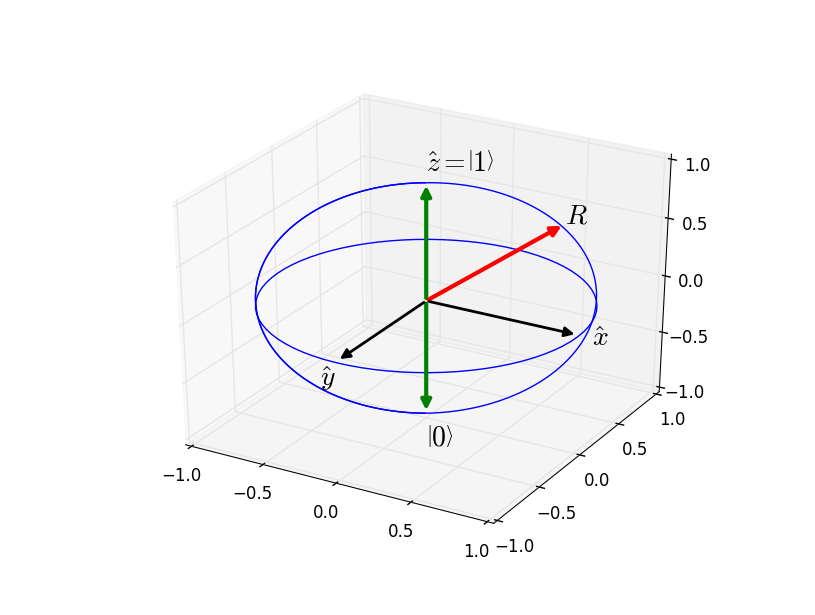
\includegraphics[width=0.7\linewidth]{Bloch_Sphere}
	\caption[Bloch sphere representation of qubit wavefunction]{Vectors on the Bloch sphere can represent any possible qubit state $\Psi = a\ket{0} + b\ket{1}$. The $\hat{z}$ axis represents $\ket{1}$, while the $-\hat{z}$ axis represents $\ket{0}$.  Positions along the equator represent equal population superpositions at different phases $\Psi = \frac{1}{\sqrt{2}}( \ket{0} + e^{i \phi} \ket{1} )$.}
	\label{fig:bloch}
\end{figure}

Rotations are a convenient basis for describing coherent operations on qubits because all decoherence-free operations will preserve $\left| a \right|^2 + \left| b \right|^2 = 1$ and will therefore merely rotate the Bloch representation of each state along the surface of the Bloch sphere.  To perform these rotations using systems with a strong dipole moment, it is only necessary to use an external electric field.  Consider the two level Hamiltonian for our qubit system
\begin{equation}
H = \frac{\hbar}{2} \omega \sigma_z \mathrm{,}
\end{equation}
where $\omega$ is the angular frequency defined above and I have used $\sigma_z$, one of the three Pauli matrices
\[ 
\sigma_x = \left( \begin{array}{cc} 0 & 1 \\ 1 & 0 \end{array} \right) \quad
\sigma_y = \left( \begin{array}{cc} 0 & -i \\ i & 0 \end{array} \right) \quad
\sigma_z = \left( \begin{array}{cc} 1 & 0 \\ 0 & -1 \end{array} \right)\mathrm{.}
\]
We can generally describe coherent interaction of this two level system with an external electric field via the potential
\begin{equation}
	V = \left| \vec{\mu} \cdot \vec{E} \right| \cos{\left( (\omega + \delta) t \right)} \sigma_x \mathrm{,}
\end{equation}
where $\vec{\mu}$ is the ion dipole moment, $\vec{E}$ is the electric field magnitude and polarization, and $\delta$ is the detuning of the electric field oscillation angular frequency from $\omega$.

Consider a qubit system initialized to $\ket{0}$.  Using time dependent perturbation theory, we can find the time derivatives of $a$ and $b$ to be 
\begin{eqnarray}
	\label{eqn:dota}
	\dot{a} &=& -i \Omega b e^{i \delta t} \\
	\label{eqn:dotb}
	\dot{b} &=& -i \Omega a e^{-i \delta t} \mathrm{,}
\end{eqnarray}
where we have dropped the quickly oscillating complex amplitudes and defined $\Omega \equiv \frac{ \vec{\mu} \cdot \vec{E} }{\hbar}$.  For short interaction times we can approximate the probability amplitudes of the two states as constant and let $a(t) \approx 1$ and $b(t) \ll 1$.  In this approximation, the population transferred to the excited state, $\ket{1}$, 
\begin{equation}
	\left| b \right| ^2 = \Omega^2 \frac{\sin^2{ \delta t / 2 }}{\delta^2} \mathrm{.}
	\label{eqn:shortpulses}
\end{equation}
This equation will be useful for using short pulses to make simple measurements of $\Omega$ in later chapters.

The above approximations hold for small population transfers, but in order to analyze the long term behavior we need to simultaneously consider both the excited and ground state occupations.  In order to make a geometric connection we can start by considering
\begin{eqnarray}
	u &=& 2\Re(a b^* e^{i \delta t}) \\
	v &=& 2\Im(a b^* e^{i \delta t}) \\
	w &=& \left| b \right|^2 - \left| a \right|^2
\end{eqnarray}
where $u$, $v$, and $w$ are the x, y, and z components of the Bloch sphere representation of $\ket{\Psi}$ with an additional rotation of the Bloch sphere at angular frequency $\delta$.  Their time derivatives can then be found using Equations~\ref{eqn:dota} and \ref{eqn:dotb} to be
\begin{eqnarray}
	\dot{u} &=& \delta v \\
	\dot{v} &=& -\delta u + \Omega w \\
	\dot{w} &=& -\Omega v
	\label{eqn:wdot}
\end{eqnarray}
Defining $\vec{P} = u \hat{x} + v \hat{y} + w \hat{z}$ to be the vector representing $\ket{\Psi}$, we can write $\dot{\vec{P}} = \vec{P} \times ( \Omega \hat{x} + \delta \hat{z} )$.  This formulation makes it clear that we can coherently control the state of a single qubit by controlling the frequency and amplitude of near resonant electric fields.  These degrees of freedom choose a vector about which the Bloch sphere representation of the qubit state will precess, and choosing the correct time duration allows us to reach any state we desire. 

If we are only interested in the probability of measuring $\ket{1}$ after beginning in $\ket{0}$, we can derive the results easily from Equation~\ref{eqn:wdot}.  The maximum probability to reach $\ket{1}$ can be found by reflecting the $-\hat{z}$ axis across the vector $\vec{W} = \Omega \hat{x} + \delta \hat{z}$, and the rotation speed is determined by the length of $\vec{W}$.  The transition is driven with probability
\begin{equation}
	\left| b \right|^2 = \frac{\Omega^2}{W^2} \sin^2( W t / 2 )
\end{equation}
where we have defined
\begin{equation}
	W^2 \equiv \Omega^2 + \delta^2 \mathrm{.}
\end{equation}
By applying resonant ($\delta$ = 0) electric fields, we see that we can cause population to fully oscillate between $\ket{0}$ and $\ket{1}$.  This behavior is called Rabi oscillation and $\Omega$ is often referred to as the Rabi frequency.  Simply controlling the exposure time of the fields to the ion allows us to perform an arbitrary rotation around the $\hat{y}$ axis on the Bloch sphere.  Given the strength of these couplings in ions, full population transfers can easily be achieved in 1~$\mu$s to 10~$\mu$s with readily available optical or rf power.  By controlling the detuning of the field or by allowing some phase evolution between the field and qubit, we can perform rotations about $\hat{z}$.  Combining the two we can easily implement the H and T gates, or any other set of single qubit gates that we need.

However, the fundamental speed increases available through quantum computation rely on the ability to generate entanglement between qubits.  Without entanglement a quantum computer will not be able to outperform a classical, probabilistic computer.  Therefore, we must have at least one operation which can generate entanglement between our qubits.  A common choice is the controlled NOT operation, which is described by the unitary matrix given in Equation~\ref{eqn:univgates}.  The corresponding classical action can be described as flipping the state of the controlled qubit if the other qubit is set to $\ket{1}$, and otherwise doing nothing.

While single qubit operations are relatively easily engineered in trapped ion systems, implementing entangling operations is significantly more difficult.  The method used to implement them is dependent on the interaction that can be engineered between the qubits themselves.  In trapped ion systems, $N$ ions that are confined in the same trap share $3N$ quantum harmonic oscillator modes of motion coupled via Coulomb forces.  These harmonic oscillator states are used as intermediate states to allow communication between the qubits.  A number of methods for generating entanglement between ions have been proposed including the Cirac-Zoller gate \cite{Cirac:95}, the M{\o}lmer-S{\o}rensen gate \cite{Sorensen:00}, and the Garc\'{i}a-Ripoll gate \cite{GarciaRipoll:03}.  The Garc\'{i}a-Ripoll gate has the most desirable properties including being completely insensitive to the ions motional energy and having a total gate time that can be much quicker than the time scale of the motion of the ions.  However, the optical setup to efficiently implement it is complicated \cite{Mizrahi:13}, and we will instead use the M{\o}lmer-S{\o}rensen gate for the moment.

\begin{figure}
	\centering
	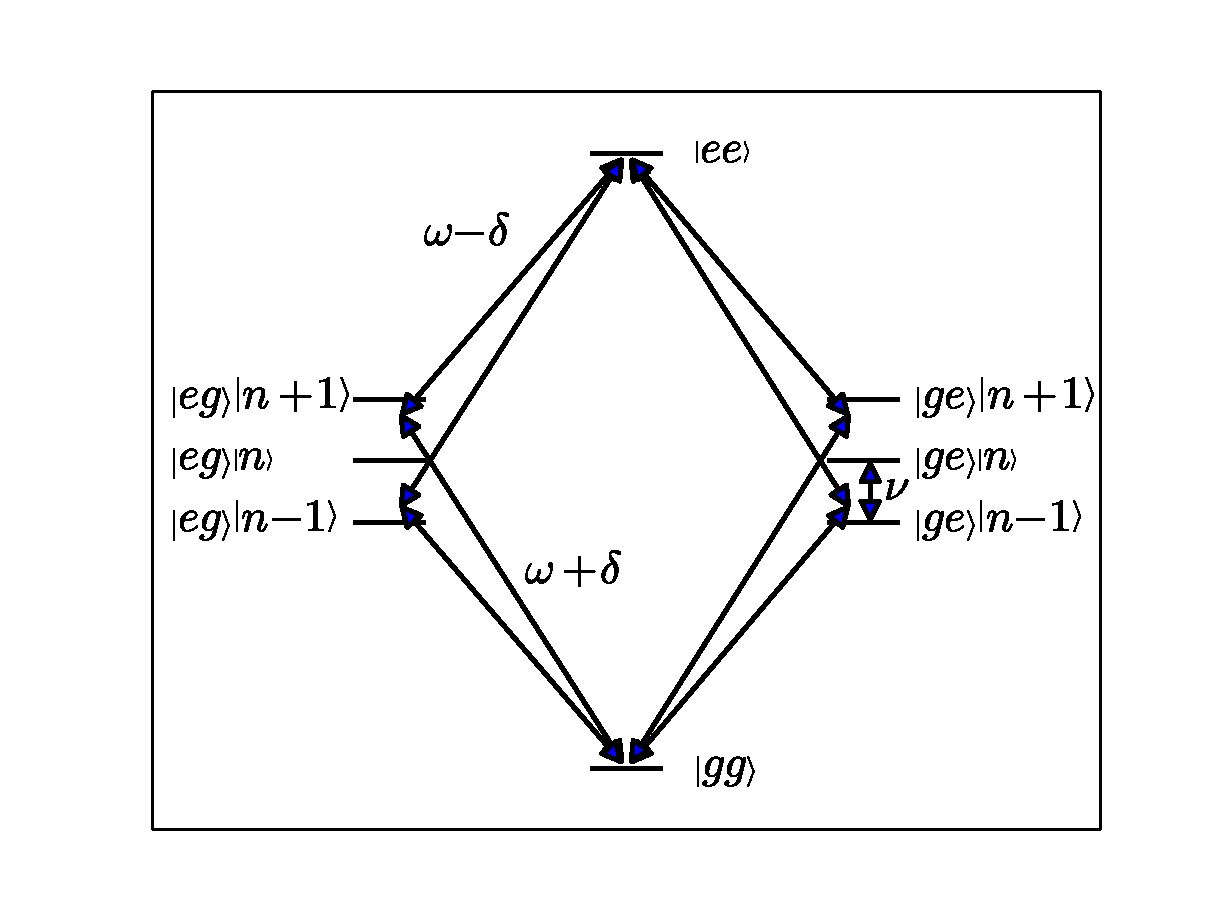
\includegraphics[width=0.7\textwidth]{MolmerSorensen}
	\caption[Diagram of M\o{}lmer-S\o{}rensen gate]{Diagram of relevant energy levels and transitions for implementing the M\o{}lmer-S\o{}rensen gate.  Two optical fields are each applied to two ions at frequencies $\omega \pm \delta$, where $\omega$ is the angular frequency splitting between the qubit levels $\ket{0}$ and $\ket{1}$.  $\delta$ is tuned near but not resonant with the motional mode angular frequency, $\omega_x$.}
	\label{fig:molmersorensen}
\end{figure}

The M{\o}lmer-S{\o}rensen gate is a two qubit entangling gate that uses these motional modes and is tolerant to finite temperature in them.  For a normal mode with angular frequency $\omega_x$ and a qubit angular frequency $\omega$, the two ions are both exposed to two external fields with angular frequencies $\omega \pm \delta$.  When $\delta$ is tuned close to $\omega_x$, these fields excite a virtual phonon into the motional mode and then remove it.  The resulting evolution of the qubit states is independent of the number of motional quanta in the mode, $n$ (for sufficiently small $n$), but the two ions are linked via the exchange of the phonon and must coherently transition together.  The action of this pulse sequence on two qubit states of our qubit levels, $\ket{0}$ and $\ket{1}$, can be described by
\begin{eqnarray}
	\ket{00} &\rightarrow& \cos\left( \frac{\Omega_{MS} t}{2} \right) \ket{00} + i \sin\left( \frac{\Omega_{MS} t}{2} \right) \ket{11} \\
	\ket{11} &\rightarrow& \cos\left( \frac{\Omega_{MS} t}{2} \right) \ket{11} + i \sin\left( \frac{\Omega_{MS} t}{2} \right) \ket{00} \\
	\ket{01} &\rightarrow& \cos\left( \frac{\Omega_{MS} t}{2} \right) \ket{01} - i \sin\left( \frac{\Omega_{MS} t}{2} \right) \ket{10} \\
	\ket{10} &\rightarrow& \cos\left( \frac{\Omega_{MS} t}{2} \right) \ket{10} - i \sin\left( \frac{\Omega_{MS} t}{2} \right) \ket{01} 
\end{eqnarray}
where we have defined
\begin{equation}
	\Omega_{MS} = \frac{(\Omega \eta)^2}{\delta - \omega_x}\mathrm{,}
\end{equation}
and $\Omega$ is the coupling strength of the field to the qubit transition as in Equations~\ref{eqn:dota} and ~\ref{eqn:dotb}, while $\eta = \sqrt{\frac{\hbar}{2 m \omega_x}} k_x$ is the Lamb-Dicke parameter that describes the coupling strength between the photon momentum and each ion's motional states in terms of the ion's mass, $m$, and the photon wavevector in the $\hat{x}$ direction, $k_x$.  Since this transition is independent of the motional energy level of the ion, it can be driven with relatively high temperatures that can easily be reached with simple laser cooling techniques.  The entanglement is even robust against ion heating during the transition and only requires that the ion be cold enough to satisfy $\eta^2 n \ll 1$.  This type of gate has been successfully performed with reasonable fidelities in ion traps \cite{Hayes:12,Hayes:10}.  The M{\o}lmer-S{\o}rensen gate implements an entangling operation, but it is not the easily described CNOT operation from above.  However, by performing single qubit rotations before and after this entangling operation, CNOT gates can be realized.
	
Implementing a quantum algorithm can be thought of as applying a complicated unitary matrix on a number of initialized input and ancillary qubits.  The Solovay-Kitaev algorithm allows us to approximate any such quantum algorithm we want to perform using a sequence of operations drawn from a universal set of quantum gates \cite{Dawson:06}.  This algorithm allows us to construct an approximation with error at most $\epsilon$ to any unitary matrix using a number of simple gates that scales as $\log^2(1 / \epsilon )$.  The approximation can be found efficiently on a classical computer before the algorithm is implemented on a quantum device.  For this reason, we can only concern ourselves with implementing the H, T, and CNOT gates I have described, with the promise that by performing many of these gates we can approximate any algorithm.  The only problem with this course of action is the accumulation of errors by performing millions of these simple gates.  Error rates $<$ 10$^{-4}$ have been demonstrated for single qubit gates in trapped ion systems \cite{Brown:11}, but lower rates will be necessary for more than a few thousand gates.  For complicated quantum algorithms, quantum error correction will be necessary to stop this propagation of error, and maintain the fidelity of the approximation to the algorithm in question.  Quantum error correction was first conceived of by Shor and requires more ancilla qubits for each computational qubit and more simple gates for each operation, but promises a higher total fidelity at the end of the algorithm\cite{Shor:95}.  The techniques have been adapted to many different quantum computing proposals including new, scalable architectures for trapped ions\cite{Oi:06}.

All of the basic requirements for quantum computation have been demonstrated with ion trapping systems using available technology.  The difficulty remains in scaling the number of communicating trapped ions to a sufficiently large number to outperform classical computers.  The number of required ions is not the billions it would take to compete with the number of bits in a classical computer, but instead only a few hundred to a few thousand because of the incredibly efficient quantum algorithms that are available for some difficult problems.  In Chapter~\ref{sec:musiqc}, I will discuss our strategies for reaching these numbers of communicating ions.


\chapter{Scalable Ion Trap Quantum Computation}
\renewcommand{\curdir}{musiqc}
\label{sec:musiqc}

\graphicspath{ {\curdir/Graphics/}  }

Hopefully, I have convinced you by now that trapped ions offer the potential to realize the building blocks of a quantum computer.  The difficulty in performing useful quantum computing tasks with them is then relatively easily reduced to the problem of having a sufficient number of communicating qubits available.  A single ion trap can easily confine ten ions, but as more ions are loaded into the trap difficulties begin to arise.  It becomes increasingly difficult to form stable linear chains, and once crystallized, it is more difficult to spatially address individual ions with lasers and to frequency address individual motional modes of the ions.  The motional modes become closer together in frequency and the motional amplitude per ion in each mode is reduced.  Also, the additional motional modes of the trap contribute to decoherence through off-resonant processes.  In order to build an ion trap quantum computer of useful size we will need to couple ions in separate, modular traps.

\section{MUSIQC Architecture}
\label{sec:arch}

To address these issues, a collaboration of ion trappers proposed a new architecture that works towards scalability in two ways. The architecture is known as the Modular Universal Scalable Ion-trap Quantum Computer (MUSIQC) \cite{Monroe:14}.  The first increase in scalability is to implement additional voltage degrees of freedom to improve our control of dc electric fields in ion traps.   In Figure~\ref{fig:musiqc}, this idea is represented by the many small dc electrodes near the trapped ions in the left panel.  This technology will enable us to trap additional ions in a single trapping region and to form additional trapping regions in each vacuum chamber.  In order to easily address and image ions from outside of the vacuum chamber, it is far preferable to crystallize them in a linear chain.  Therefore, their axial confining strength must be kept weaker than their radial confining strength.  The difficulty that arises is that as more ions are loaded into the same trap, the ions at the outer ends of the chain provide additional axial confinement to the center ions through Coulomb repulsion.  The result of which is that trapping increasing numbers of ions in a linear chain requires increasing amounts of radial trap strength to counteract the additional axial confinement.  Especially for heavier ions species, increasing radial strength can become difficult quickly.

\begin{figure}
	\centering
	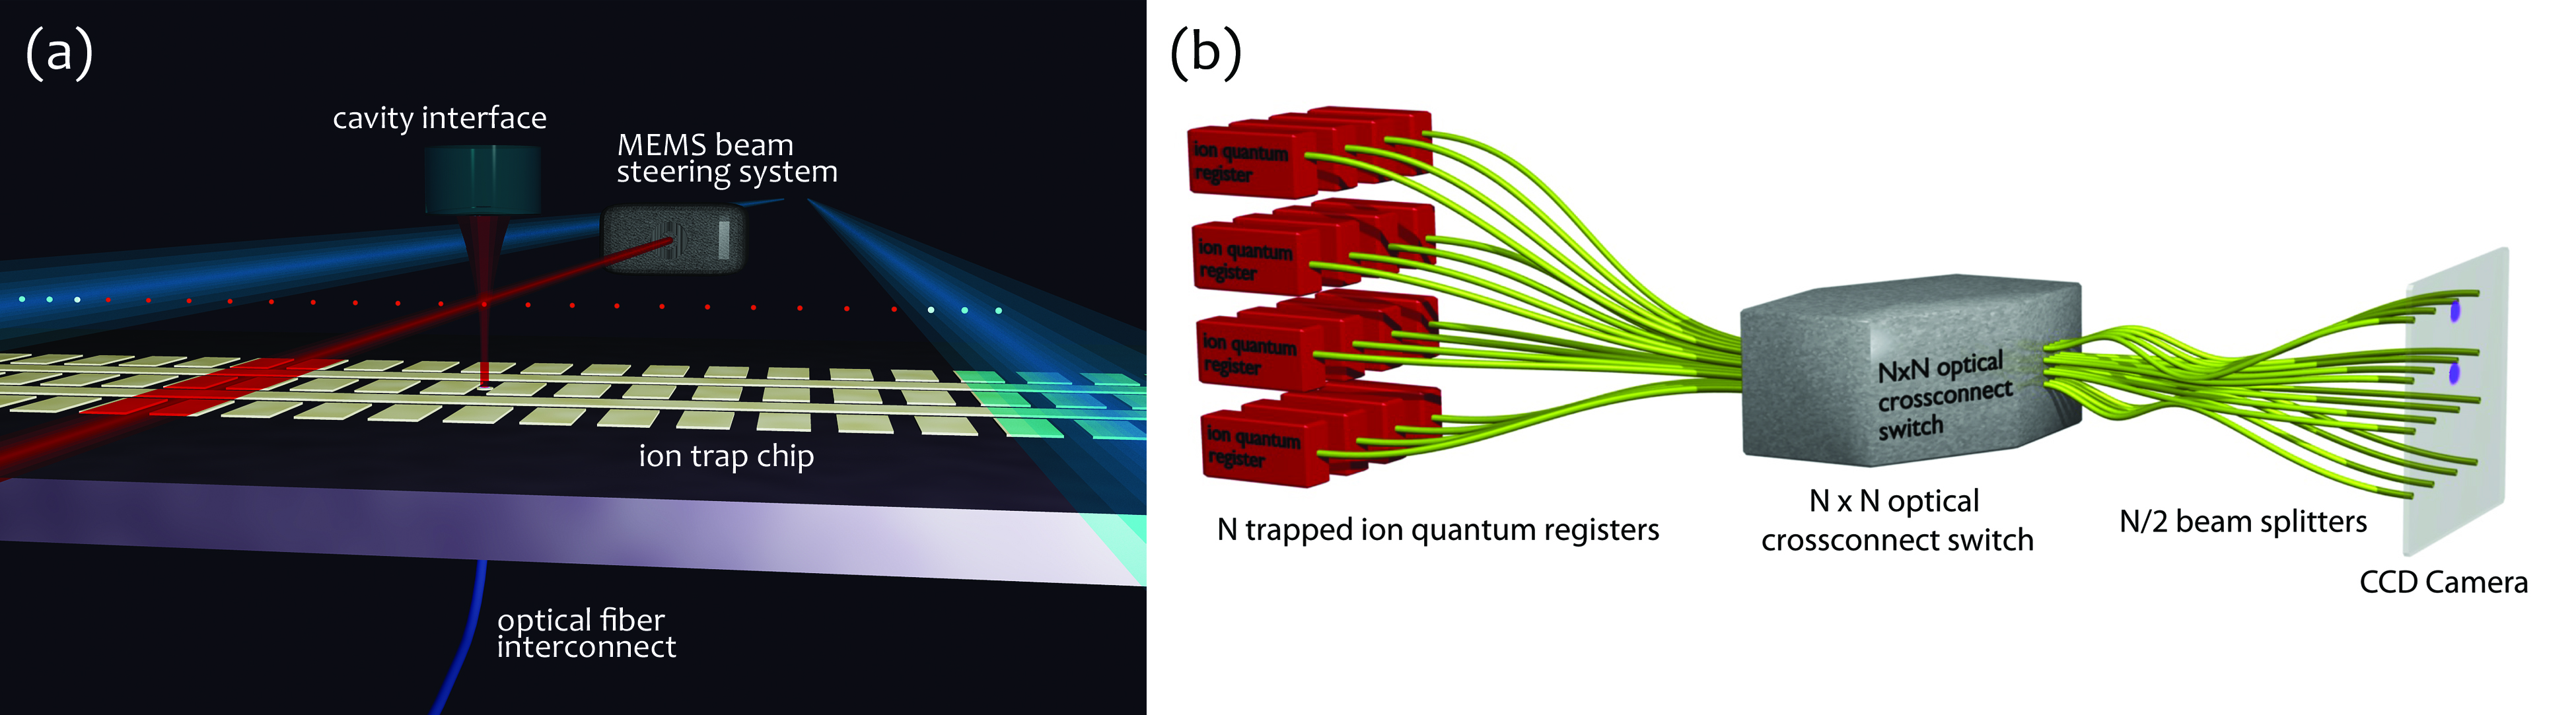
\includegraphics[width=\textwidth]{MUSIQC-plan}
	\caption[Schematic diagram of the MUSIQC architecture]{Schematic diagram of the Modular Universal Scalable Ion-trap Quantum Computer architecture.  Two species of ions are trapped in a surface ion trap with some ions coupled to optical fiber (left).  Photons in these optical fibers can be switched and interfered to generate entanglement between separate modular ion trapping systems (right).}
	\label{fig:musiqc}
\end{figure}

In order to correct for this effect, it is desirable to lower the axial confinement that the center ions experience without compromising the confinement of the entire chain.  Adding higher order anharmonic terms to the axial trap potential can reduce the increase in the axial frequency and allow more ions to be stably trapped \cite{Lin:09}.  Since ions are very sensitive to electric fields, it is easy to add additional controls to their axial potential just by adding more dc control electrodes.  In order to have many small control electrodes, ion traps that are made using standard microfabrication techniques have been developed.  These techniques have been used in the condensed matter community for decades and transfer very well to the manufacture of small ion traps.  Using these additional trap degrees of freedom we expect to be able to trap $\approx$ 20 ions in a trapping region.

Using these additional dc voltage controls, it is also possible to generate and control multiple trapping regions inside the same vacuum chamber.  In fact, generating multiple trapping locations has already been demonstrated, as well as separating ions from and merging ions into these traps \cite{Moehring:11}.  While entangling operations rely on shared motional modes between the ions and can only occur between ions in the same trapping region, entangled ions can be moved between different trapping regions without decoherence \cite{Bowler:12}.  Using these capabilities we can perform our entangling operations in traps with fewer ions and therefore fewer motional modes to improve fidelity and then shuttle the ions back to other trapping locations.  The current usefulness of this procedure is limited by a few concerns.  The separation and merging operations using our current dc control systems take several milliseconds, and the operation might be complicated depending on how many ions need to be reordered to transfer the desired information.  However, with more complicated trap geometries this idea may become more feasible in the future.

Using current surface trap designs, it is possible to store hundreds of ions inside a single vacuum chamber.  While this would be a very impressive technical demonstration, it would not be a modular system and additional scalability would be difficult.  Also, adding more trapping regions to each vacuum chamber increases the difficulty of shuttling ions between them.  All of the lasers applied to the ions need to be carefully focused and directed to avoid interacting with the many other ions inside the $\approx$ 5~mm diameter microfabricated trap.  Applying rf and microwave control fields to single ions in such systems would be very difficult because of their wavelengths, which is unfortunate because many desirable qubit levels are separated by these frequencies.   While none of these difficulties are insurmountable, a separate method of scaling our system will almost certainly prove useful.

The second way that we propose to work towards scalability is by transferring entanglement between separate microfabricated traps or even separate vacuum chambers.  Given an appropriate choice of qubit, it is very easy to generate entanglement between the qubit levels in a trapped ion and single photons \cite{Moehring:04,Stute:12}.  The resulting qubit state of an ion emitting a photon can be encoded into the frequency and polarization of the emitted photon.  The problem of coupling quantum information in ions between vacuum chambers is then reduced to the problem of coupling photons between the chambers.

Coupling photons together is a problem that has already been almost entirely solved.  Optical fiber technology is available that will transfer photons from ions with reasonable loss rates.  Any necessary operations on the photons polarization can be accomplished using optical fiber tools.  The only remaining difficulty is interconnecting the fibers of any desired pair of ion traps.  This last task can be accomplished using a custom microelectromechanical system (MEMS) of mirrors to redirect light from an input array of fibers to any desired output fibers which has already been demonstrated \cite{Olkhovets:04}.  The trapping and quantum operations apparatus can be built into a modular device, and more qubits can be connected by the system by connecting their fiber ports to the fiber switch (see the right panel of Figure~\ref{fig:musiqc}).

For reasons discussed in the next section, this photonic information transfer will be significantly slower than the timescale of other operations in the trap.  Quantum gates between ions in the same trap can usually be performed at rates of $\approx$ 100~kHz to 1~MHz.  Shuttling ions containing information between separate trapping regions can be accomplished at a rate of $\approx$ 1~kHz - 10~kHz.  Transferring quantum information between remote ions in separate vacuum chambers can currently be done at 1~Hz to 10~Hz, but we believe that we can increase this rate to $\approx$ 1~kHz.  Nevertheless, quantum algorithms will be possible using this architecture. Analysis has shown that the MUSIQC architecture compares favorably with other commonly suggested scalable quantum computer architectures \cite{Monroe:14}.  The slower remote entanglement step also does not preclude the implementation of quantum error correction.

\section{Remote Entanglement}
\label{sec:remote}

The first step to implementing this remote ion-ion entanglement procedure is collecting single photons from trapped ions.  Each modular trap system will need to feature one or more locations that are optically coupled to a single mode optical fiber.  An ion trap system that was not designed with this feature in mind will usually collect approximately 2\% of the available ion fluorescence using a long working distance microscope objective placed outside of the vacuum chamber.  The resulting probability of successfully managing to entangle two ions in distant traps in a single trial will be very small.  Attempting the entanglement and hoping that it worked is not a realistic possibility.  Fortunately, there is a protocol by which it can be determined whether the entanglement process was successful without performing a measurement that would destroy the entanglement.

First, we must simultaneously couple two single photons each entangled with an ion in separate modules.  The ion is initialized to one qubit state and then excited to a state that can decay to either qubit state by emitting a distinguishable photon (see Figure~\ref{fig:remoteentangle}).  For example, considering vacuum chambers $A$ and $B$, photon quantum states $\ket{H}$ and $\ket{V}$, and ion qubit states $\ket{\uparrow}$ and $\ket{\downarrow}$ we will generate the state
\begin{equation}
	\ket{\Psi} = \bigotimes_{i=A,B} \frac{1}{\sqrt{2}} \left( \ket{H}_{i}\ket{\uparrow}_{i} + \ket{V}_{i}\ket{\downarrow}_{i} \right)\mathrm{.}
\end{equation}
The photon states need to be some distinguishable photon states maximally entangled with the ion states.  Polarization states can be used easily or frequency states can be used if the frequency separation is larger than the linewidth of the transition.  We can then overlap the photon spatial modes on a 50-50 beamsplitter at some other location.  When single photon detectors placed at both output ports of the beamsplitter are simultaneously triggered that will correspond to measuring the photon state as $\frac{1}{\sqrt{2}} \left( \ket{H}_A\ket{V}_B - \ket{V}_A\ket{H}_B \right)$.  If the photons were both in $\ket{H}$ or both in $\ket{V}$, the probabilities of both photons reflecting off the beamsplitter or both transmitting through the beamsplitter interfere and the photons must both be output on the same interferometer arm.  We can determine the resulting state of the ion by projecting the measured photon state onto $\ket{\Psi}$.  The ions are left in the state
\begin{equation}
	\ket{\Psi}_\mathrm{ion} = \frac{1}{\sqrt{2}} \left( \ket{\uparrow}_A \ket{\downarrow}_B - \ket{\downarrow}_A \ket{\uparrow}_B \right)
\end{equation}
which is a maximally entangled state of the ion qubits.  This procedure destroys the initial qubit state of the ions, but remotely entangled qubits can be prepared in advance and used a resource during the computation.

\begin{figure}
	\centering
	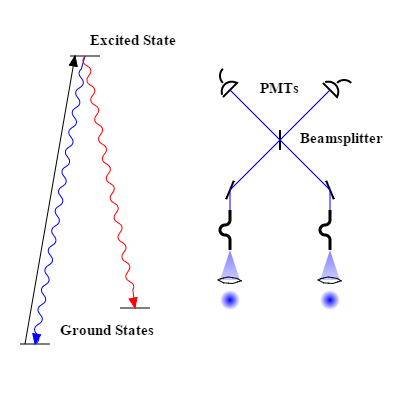
\includegraphics[width=0.6\textwidth]{remote-entanglement}
	\caption[Remote ion-ion entanglement procedure]{Diagram of the remote ion-ion entanglement experiment.  An ion is excited to a state with two possible photon decay paths (left).  The photons are collected and interfered before being detected on two PMTs (right).  The overlap of the spatial modes removes the which-path information from the system before the detection and leaves the ions entangled.}
	\label{fig:remoteentangle}
\end{figure}

Successful remote ion-ion entanglement in small scale systems with other ion species has been successfully demonstrated \cite{Matsukevich:08}.  We have begun generating entangled ion-photon pairs and are working towards a remote ion-ion entanglement demonstration using barium ions \cite{Auchter:14}.  In any given attempt an entangled ion-photon pair can be generated with probability $P$ given by,
\begin{equation}
	P = P_\mathrm{exc} f  \eta \frac{\Omega}{4 \pi} f_\mathrm{gate} T
\end{equation}
where $P_\mathrm{exc}$ is the probability of driving the transition to the excited state ($\approx$ 0.2 in our current experimental setup), $f$ is the branching ratio back to the initial state if other decays are possible ($\approx$ 0.75), $\eta$ is the quantum efficiency of the single photon detector ($\approx$ 0.2), $\Omega$ is the solid angle for the collection optics ($\approx 0.02 \times 4 \pi$), $f_\mathrm{gate}$ is the fraction of emitted photons in our detection window ($\approx$ 0.8), and $T$ accounts for other losses including transmission through all other optics ($\approx$ 0.3).  These factors currently limit us to generating an entangled ion-photon pair at about 2.5~Hz given our 17~kHz repetition rate \cite{Auchter:14}.  

Generating an entangled ion-ion pair requires the simultaneous generation of two ion-photon pairs which means that it only succeeds with probably proportional to $P^2$.  The photons must also be transmitted through a length of optical fiber, have their spatial modes overlapped, and be in a correct state to allow the heralded entanglement scheme to occur, but these factors are insignificant or unavoidable.  The largest achievable gains in our apparatus would be to $P_\mathrm{exc}$ which can easily be increased to unity, and $\Omega$ which can be increased by a factor of 5 to 10.  The MUSIQC collaborators are exploring a number of possible methods to improve $\Omega$ including in vacuum cavities \cite{Sterk:12} and diffractive optics \cite{Clark:14}.  We have designed and built an ion trap inside of a parabolic mirror which can be used to collect $\ge 40\%$ of an ion's fluorescence \cite{Shu:11}, and we are working to implement ion-ion entanglement experiments in that system.  Using currently available technology, we believe a remote ion-ion entanglement rate of $\approx$ 1~kHz is feasible and we are working towards achieving that goal.

\section{Mixed Ion Species}
\label{sec:mixed}

Unfortunately, as the implementation of this scheme proceeded, field crosstalk between neighboring ions was a problematic issue.  The generation of remote entangled ion pairs requires the application of resonant laser beams on strong transitions.  Even with ion separations of 10~microns, well focused lasers can still scatter hundreds of photons per second from neighboring ions.  Scattering any photon will completely destroy the quantum information that might have previously been held in the ion, and can quickly disrupt an entire calculation.  The determination was eventually made that we needed to take measures to avoid this problem.

\begin{figure}
	\centering
	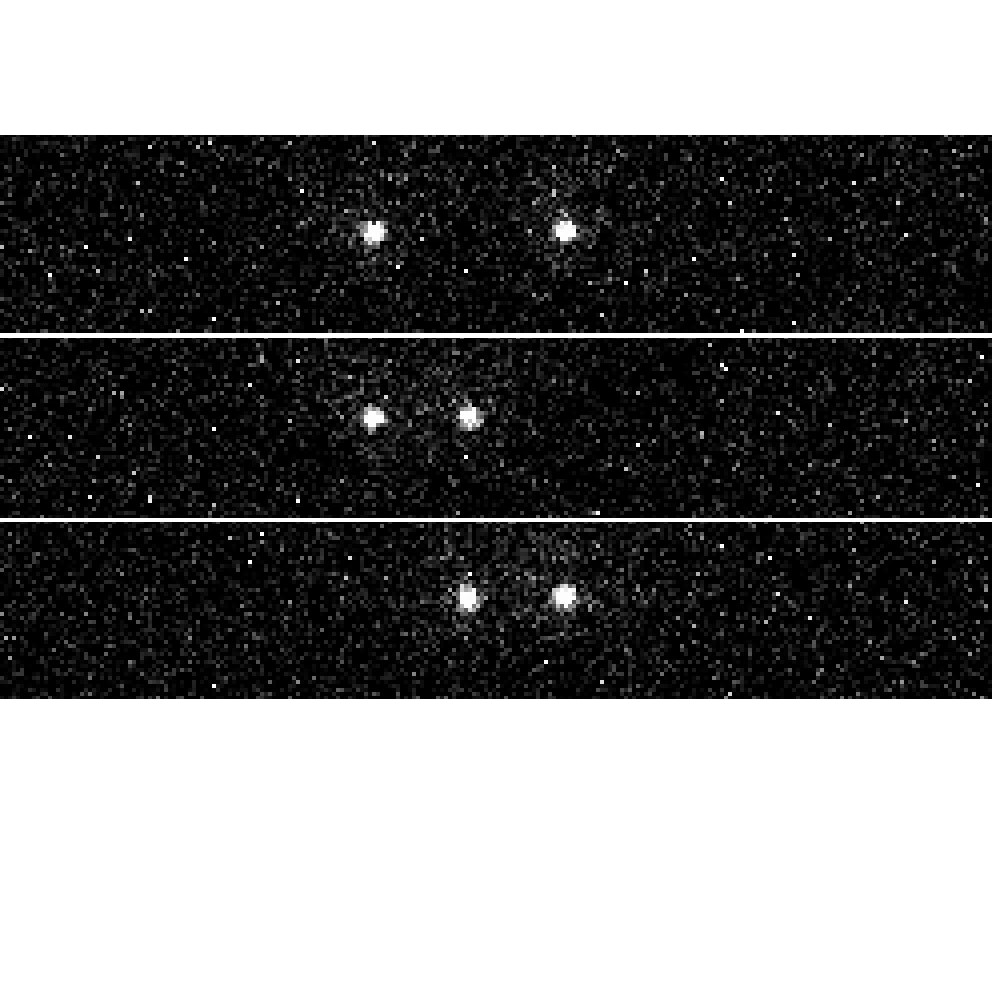
\includegraphics[width=0.6\textwidth]{BaYb}
	\caption[CCD image of barium and ytterbium ions]{CCD image of two barium and a ytterbium ion in the a linear ion crystal.  Fluorescence from the barium ions is visible, while the ytterbium ion is dark.  The ytterbium ion is in the center in the top panel, the left in the middle panel, and the right in the bottom panel.}
	\label{fig:bayb-ccd}
\end{figure}

The method chosen to minimize the field crosstalk issue was to use separate ion species for quantum computation and the remote entanglement generation.  This choice cements the idea of remote entangled pairs as a computational resource.  One ion species can be dedicated to generating many entangled pairs that can be transferred into the computation by quantum teleportation of the entanglement onto the computational ion species.  Only the computational ion species will store quantum information for any significant period of time or perform any calculations with it.  Previous work towards a similar mixed ion species system has been done with small numbers of ions already \cite{Lin:13}.

Another advantage of adopting this scheme is that there are now many ions motionally coupled to the computational ions, but with well-separated optical transition frequencies.  Laser cooling can be performed on the remote entanglement species with a negligible chance of scattering a photon from the computational ions.  Since the two species are motionally coupled, it should be possible to keep the entire chain of ions cold without affecting ongoing quantum algorithms.  By using quantum gates that are insensitive to small motional occupation numbers and electromagnetically-induced-transparency cooling \cite{Lin:13, Roos:00}, it may even be possible to avoid ever having to laser cool the computational ions.  This would allow quantum algorithms to continue running until qubit begins to decohere instead of being forced to stop by heating issues as is often the case.  The use of the M{\o}lmer-S{\o}rensen gate discussed in Chapter~\ref{sec:qcomp} is also helpful here because of its resistance to decoherence even when performed at finite ion temperatures and during ion heating.  

The added difficulty in only laser cooling one species is that different ion species obviously have different masses, which causes each normal mode of the chain to couple more strongly to one ion species than the other.  For large mass differences, this imbalance can make it impossible to cool one ion species using the other.  Each mode will have eigenvector components of order one with one ion species and all of its eigenvector components with the other ion species may be $\le$ 0.01 or even less.  The result is that even with large amounts of energy in this mode, the ion species being laser cooled may have very little motion.  

It is hoped that by choosing ion species with small mass differences and by exploring other degrees of freedom, this cooling scheme may be possible.  These other degrees of freedom include number and arrangement of the cooling ions and overall trap strengths and anharmonicities.  After going through our ion trapping, cooling, initialization, and readout procedures in more detail in Chapters~\ref{sec:trap} and \ref{sec:ioncool}, I will explore these ideas further.

The two ion species that will be used for the MUSIQC program are ytterbium and barium.  We have already successfully trapped these two species in the same linear ion chain (see Figure~\ref{fig:bayb-ccd}).  Ytterbium-171 has a pair of ground state levels with excellent insensitivity to magnetic fields.  These levels have very long coherence times and the state of the ion can be determined using a simple optical setup.  Barium has the advantage of having a strong transition at 493~nm, which is a long wavelength transition among ion species that can be laser cooled.  This wavelength is transmitted through fibers easier than more ultraviolet transitions which will improve the rate at which remote entangled pairs can be generated.  Further the two species are relatively close in mass, which should help to improve their motional coupling.




\part{Trapping Barium and Ytterbium Ions}

\chapter{Linear and Surface RF Traps}
\renewcommand{\curdir}{trap}
\label{sec:trap}

\graphicspath{ {\curdir/Graphics/}  }

Basic electrostatics requires that in free space the electric potential $\phi$ obey
\begin{equation}
	\nabla^2 \phi = 0
\end{equation}
and therefore it is impossible to have $\partial_x^2 \phi > 0$, $\partial_y^2 \phi > 0$, and $\partial_z^2 \phi > 0$ at the same point in space, which is the condition for having a stable trap in three dimensions for a positively charged particle.  The best possibility with electrostatics is to form a trap in two dimensions, but the third axis will always be an unstable equilibrium point.

Therefore to stably confine a charged particle, we have to use either static magnetic fields or time-varying electric fields.  Both of these possibilities are used in modern labs, but working with magnetostatics in Penning traps requires that the ions precess about the magnetic field axis which makes performing quantum operations on them more difficult.  All control lasers and readout must be continuously corrected for the rotation \cite{Sawyer:12,Britton:12}.  These traps are often used for precision measurements in fundamental physics \cite{Blaum:10}.  Most quantum information efforts with trapped ions use linear rf traps, which use radio frequency and dc electric fields to generate stable trapping \cite{Paul:90}.  Linear rf traps allow stationary confinement of any charged particle.

In order to more rapidly evaluate different ion trap designs, we have been working on two separate traps in different vacuum chambers.  Power from all of the necessary ionization and cooling lasers is split between the two traps.  Both chambers were originally designed to hold microfabricated surface traps, but one has been converted to hold a standard macroscopic linear rf trap in order to more easily test new quantum operations.

\section{Linear RF Traps}
\label{sec:paul}

\begin{figure}
	\centering
	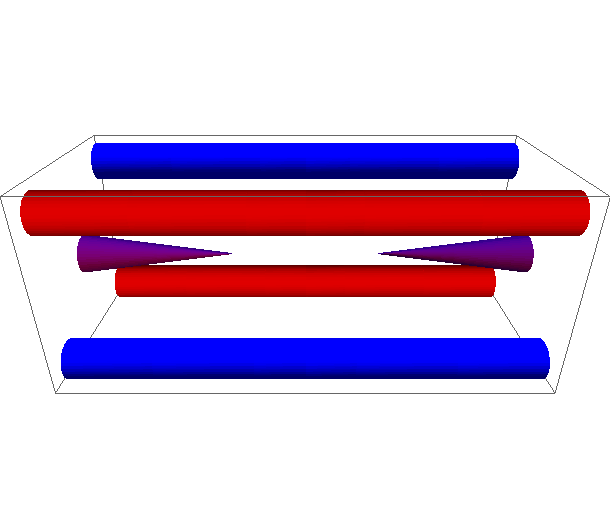
\includegraphics[width=0.8\linewidth]{PaulTrap}
	\caption[Schematic drawing of a linear rf trap]{Schematic drawing of a linear rf trap.  Radial confinement is provided by applying high voltage rf to the red rods while the blue rods are held at ground. Axial confinement is generated by applying high voltage dc to the purple needles.}
	\label{fig:paultrap}
\end{figure}

The easiest linear rf trap geometry to understand features four long rods arranged in a square with their long axis along z (see Figure~\ref{fig:paultrap}).  Radio frequency voltage is applied to two rods in opposite corners (red) and the other two rods are grounded (blue).  The rods provide radial confinement for the ions, and axial confinement is then provided by applying high voltage dc to two electrodes centered between the rods at opposite ends (purple).

At the center of the trap the rods form an oscillation radial quadrupole electric field that is a function of the angular frequency of the applied rf, $\Omega_\mathrm{rf}$, the amplitude of the rf voltage, $V_\mathrm{rf}$, and a geometrical constant, $\kappa_\mathrm{rf}$.  The resulting potential is
\begin{equation}
	\Psi_\mathrm{rf} = \kappa_\mathrm{rf} V_\mathrm{rf} \cos( \Omega_\mathrm{rf} t ) \left( x^2 - y^2 \right) \mathrm{.}
	\label{eq:pot_rf}
\end{equation}
The dc electrodes form a stable trap in the z (axial) direction, and an unstable equilibrium in x and y.  The electric potential caused by the dc electrodes at the center of the trap is
\begin{equation}
	\Psi_\mathrm{dc} = \kappa_\mathrm{dc} V_\mathrm{dc} \left( z^2 - \frac{1}{2} \left( x^2 + y^2 \right) \right) \mathrm{,}
	\label{eq:pot_dc}
\end{equation}
where $V_\mathrm{dc}$ is the dc voltage applied to both needles and $\kappa_\mathrm{dc}$ is a geometrical constant.  

The resulting axial trap frequency can easily be derived from Equation~\ref{eq:pot_dc} and is 
\begin{equation}
	\omega_z = \sqrt{ 2 \kappa_\mathrm{dc} V_\mathrm{dc} q / m }
	\label{eqn:axialfreq}
\end{equation}
for an ion of charge $q$ and mass $m$.  The equation of motion for one of the radial directions, $\hat{x}$, can be converted to the standard form of the Mathieu equation
\begin{equation}
	\frac{d^2 x}{d \xi^2} + (a_x + 2 q_x \cos(2 \xi)) x = 0 \mathrm{,}
\end{equation}
with the definitions
\begin{eqnarray}
	\xi &\equiv& \Omega_\mathrm{rf} t / 2 \\
	a_x &\equiv& \frac{4 q \kappa_\mathrm{dc} V_\mathrm{dc}}{m \Omega_\mathrm{rf}^2} \\
	q_x &\equiv& \frac{2 q V_\mathrm{rf}}{ \Omega_\mathrm{rf}^2 m } \mathrm{.}
\end{eqnarray}
Typically in experimental conditions we will have $a_x < q_x^2 \ll 1$, which results in a stable solution of the Mathieu equation.  The motion of the ion under these approximations can be written as
\begin{equation}
	x(t) = A_x \cos( \omega_x t + \phi_x ) \left( 1 + \frac{q_x}{2} \cos(\Omega_\mathrm{rf} t) \right) \mathrm{.}
	\label{eqn:mathieu-soln}
\end{equation}
The radial secular frequencies, $\omega_x$, correspond to the angular frequency of the harmonic oscillator potential the ion feels and are defined as 
\begin{equation}
	\omega_x \equiv \frac{\Omega_\mathrm{rf}}{2} \sqrt{ \frac{a_x + q_x^2/2}{1 - 3 q_x^2 / 8} } \mathrm{.}
	\label{eqn:radialfreq}
\end{equation}
The $A_x$ parameter is an amplitude set by the initial conditions of the ion.  There is still some residual motion of the ion at the frequency of the applied rf, $\Omega_\mathrm{rf}$, but the quantized motion of the ion is only described by $\omega_x$.  All of the above arguments carry through for both radial directions although I've only been discussing $\hat{x}$.  However, it is undesirable to have the radial frequencies be extremely close together because the resulting low frequency beat note makes the ions sensitive to low frequency electric field noise.  Therefore, $\omega_x$ and $\omega_y$ are usually separated either by slightly perturbing the radial symmetry of the geometry or by applying a radial symmetry-breaking dc field.

In Figure~\ref{fig:mathieu}, a solution to the Mathieu equation given a starting location near the trap center is shown.  Fast motion at the applied rf frequency, $\Omega_\mathrm{rf}$, is visible as well as the slower confining oscillation at the secular frequency, $\omega_x$.  These fast oscillations are known as trap micromotion and should be minimized as much as possible.  They lead to Doppler frequency sidebands on all lasers applied to the ion and increase ion heating when ions are moved by changing dc electrode voltages.  Additional micromotion is also induced when the ions are pushed off the quadrupole null by stray electric fields.  We will analyze micromotion further in Section~\ref{sec:secfreqs} when we work towards characterizing the secular frequencies and stray fields of a surface trap.

\begin{figure}
	\centering
	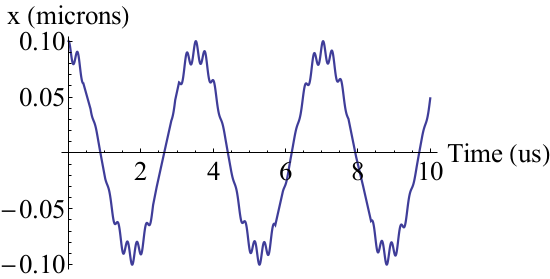
\includegraphics[width=0.8\linewidth]{PaulTrap-ion_motion}
	\caption[Sample trapped ion motion from the Mathieu equation]{Sample trajectory for an ion trapped in a linear rf trap.  The Mathieu equation is numerically integrated from a starting location near the trap center. Slow oscillation at the secular frequency and fast, driven micromotion are visible.}
	\label{fig:mathieu}
\end{figure}

When with standard macroscopic linear rf traps we have used a design exactly as pictured in Figure~\ref{fig:paultrap}.  The trap is formed by four 0.017~in (430~micron) diameter tungsten rods separated by approximately 800~microns.  The rods are held in place at either end of the trap by an alumina spacer.  In order to provide axial confinement two tungsten needles were created by electrochemically etching a fine point onto tungsten rods.  These needles are also inserted into the alumina spacers and everything is secured with a UHV-compatible cement (Sauereisen Ceramic Cement No. 8).

The rods and needles are connected to an 8-pin vacuum feedthrough.  High voltage rf to generate the trapping potential is created using a helical can resonator \cite{Siverns:12}.  Two long pieces of 3~mm diameter copper tubing are wound into a double helix of $\approx$ 4~cm diameter and 15 turns and held in the center of a 7.5~cm diameter copper can.  One end of each copper helix is connected to an rf ground and the other is connected to the vacuum feedthrough.  Rf is coupled into the resonator using a small induction coil placed inside the double helix. The shape and length of this coil can be manipulated to match the load to the standard 50~$\Omega$ output impedance of a rf amplifier.

The ground electrodes of the trap and the ends of the helix coils after the rf grounds are connected to precision dc voltage sources.  By adjusting the dc voltage of these four rods we can control the radial dc field in the trap.  These degrees of freedom allow us to cancel out any radial stray field that may be present in the trap as well as break the radial symmetry of the trap to separate the radial secular frequencies.

Although the effects of the rf are easiest to see in this type of linear rf trap geometry, many different rf and dc electrode geometries are possible.  The only requirements for this kind of trapping to work are an oscillating quadrupole electric field overlapped with dc confinement in the other directions of the correct magnitudes to correspond to a stable solution of the Mathieu equation.  A particularly simple electrode geometry is applying rf to a metal ring with dc electrodes above and below it.  Another geometry used in our group applies rf to a large parabolic mirror with a grounded metal needle inside of it \cite{Shu:11}.  The position of the ion can be manipulated by moving the needle, and by positioning it at the focus of the parabolic mirror very large fractions of the light emitted by the ion can be collected.

\section{Surface Traps}
\label{sec:surface}

A favorable geometry for working towards scalable quantum computing is called a surface electrode trap.  In this geometry, all of the electrodes are placed in a single plane.  Surface electrode traps have several advantages over standard three dimensional linear rf traps, including repeatable manufacturing processes and many separately controllable dc electrodes.  These electrodes allow the creation of separate trapping regions as well as shuttling between the regions and splitting and merging ions into them.  Many groups have been developing the techniques to design and manufacture these traps \cite{Allcock:12, Daniilidis:11, Wright:13}.

\begin{figure}
	\centering
	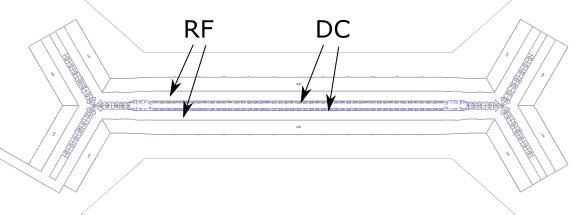
\includegraphics[width=\textwidth]{HOA}
	\caption[Electrode structure of Sandia National Lab's ``High Optical Access'' surface trap]{Electrode structure of the ``High Optical Access'' (HOA) surface trap manufactured by Sandia National Labs.  Rf voltage is applied to the long electrodes shown in red to provide radial confinement along all 5 arms of the trap.  Axial confinement is provided by applying dc voltages to the segmented electrodes between the rf electrodes.}
	\label{fig:sandia-hoa}
\end{figure}

Georgia Tech Research Institute and Sandia National Labs have provided us with microfabricated surface traps for evaluation.  The MUSIQC collaboration has been exploring a number of additional features that can be engineered into surface traps including regions of high optical access to allow tightly focused lasers, regions with optical cavities to increase ion fluorescence collection, and junctions between linear trapping regions that allow chains with different ion species composition and ordering to be organized.  Figure~\ref{fig:sandia-hoa} shows a schematic diagram of the electrodes on the trap we are currently using, the ``High Optical Access'' (HOA) trap designed and built by Sandia National Labs.  It features two junctions that allow ions to be reordered and a region in the middle where the width of the trap surface has been minimized to allow tightly focused lasers to be applied to ions from the side without clipping the trap surface.  In order to be able to evaluate different trap designs quickly we have designed and implemented a vacuum chamber that allows for quick trap replacement \cite{Graham:14}.

The surface electrode traps we receive are wirebonded onto a CPGA-100 carrier.  This carrier slots into a UHV-compatible Zero Insertion Force (ZIF) socket in the center of our vacuum chamber (see Figure~\ref{fig:chipchamber}).  The ZIF socket connects to a custom PCB that can, if necessary, host additional filtering for the dc voltages that will be applied to the trap.  The PCB also routes the connections from the socket to four 25~pin D-Sub connectors that are connected through a vacuum feedthrough to our control electronics.  The neutral atom ovens mount below the PCB.  The bottom flange of the vacuum chamber can be removed to replace the oven, and the top flange can be removed to replace the trap.  This system has been cycled from atmospheric pressure to pressures below 5~$\times$~10$^{-11}$~torr more than ten times, often in a week or less.

In order to minimize the deposition of metallic barium and ytterbium from the ovens on the back of the surface trap we have developed several techniques to shutter the ovens in the vacuum chamber.  The shutter can be activated before running the oven at very high temperatures to remove material deposited during the bake out of the UHV chamber.  These high temperature runs are necessary before the oven will produce a usable flux of the element to be ionized.  We have seen evidence that during these runs barium ovens can eject pieces large enough to completely block the loading holes on surface electrode traps.  The shutter shown in Figure~\ref{fig:chipchamber} is made of a small metal plane attached to a bimetallic strip that curls when its temperature is increased.  By running several amperes of current through the bimetallic strip the plane can be actuated to block flux from the oven below the surface trap.

\begin{figure}
	\centering
	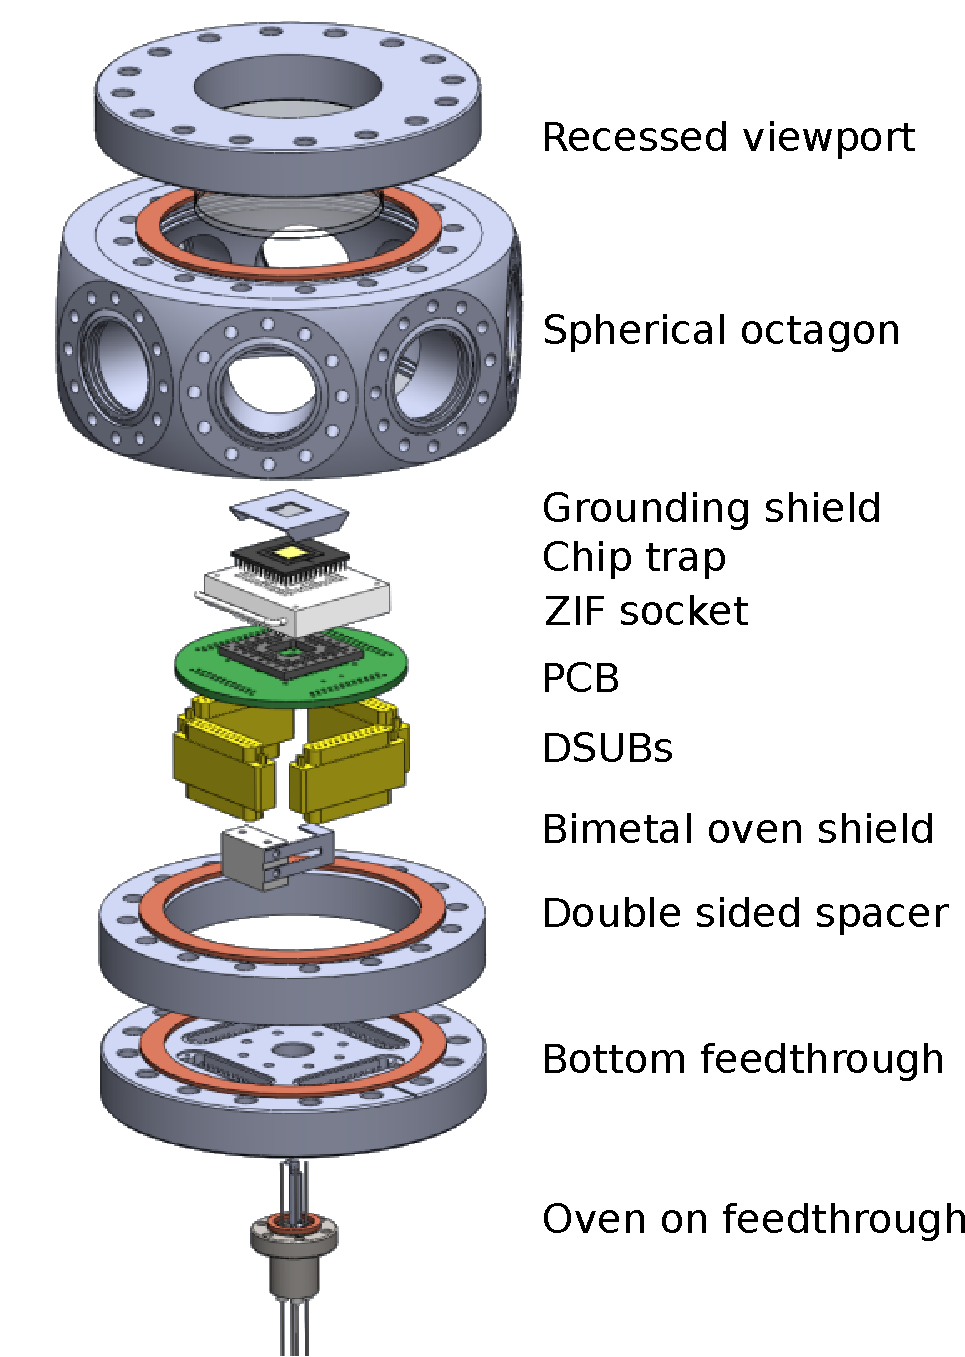
\includegraphics[width=0.7\textwidth]{chiptrap-chamber}
	\caption[Diagram of surface trap vacuum chamber]{Diagram of vacuum chamber designed for working with surface traps.  The surface trap mounts in a ZIF socket and its electrical connections are routed through 4 25-pin D-Sub connectors.  Barium and ytterbium ovens are located below the trap and can be blocked with a bimetal shutter.}
	\label{fig:chipchamber}
\end{figure}

The next step to begin working with these microfabricated traps is to calculate the correct voltage to apply to each dc electrode to generate a stable axial trap.  The electric fields at the trapping location in surface traps as a function of the applied dc voltages are often calculated using the Boundary Element Method (BEM).  All of the surfaces in the trap are subdivided into small triangles or quadrilaterals and a surface charge degree of freedom is placed at each vertex of this mesh.  In the lowest order approximation, the actual surface charge is assumed to be the linear interpolation of the surface charge at these points. These steps reduce the problem from one large integral to the sum of a large number of integrals that depend linearly on the surface charge at each vertex.  In other words, the problem of solving for the electric potential, $\phi$, is changed from
\begin{equation}
	\phi(x) = \int_{\{S\}} \frac{\sigma(x')}{4 \pi \epsilon_0 \left| x - x' \right| } dx' \mathrm{,}
\end{equation}
where $\sigma(x)$ is the surface charge density and $\{S\}$ is the set of surfaces in the trap, to the more numerically tractable
\begin{equation}
	\phi(x_i) = \sum_{S_k = x_q, x_r, x_s} \int_0^1 \int_0^v \frac{(1-u-v)\sigma(x_q) + u\sigma(x_r) + v\sigma(x_s)}{4 \pi \epsilon_0 \left| x_{S_k}(u, v) - x_i \right| } \left| \frac{\partial x}{\partial (u,v)} \right| du dv \mathrm{,}
\end{equation}
where $u$ and $v$ are a linear parametrization of the small triangular surface $S_k$, defined by the three vertices $x_q$, $x_r$ and $x_s$, such that $x_{S_k}(0, 0) = x_q$, $x_{S_k}(1, 0) = x_r$, and $x_{S_k}(0, 1) = x_s$.  The $S_k$ triangles are chosen to approximate the surfaces $\{S\}$ to the desired level of accuracy.  The desired solution is then a set of $\sigma(x_i)$ given a desired set of voltages on each surface $\phi(x_i)$ where both of these functions are only evaluated at the vertices of the mesh.

The problem of solving for these vertex surface charges can then be reduced to linear algebra by computing the integrals 
\begin{eqnarray}
	U_{ij} &=& \int_0^1 \int_0^v \frac{u}{4 \pi \epsilon_0 \left| x_{S_j}(u, v) - x_i \right| } \left| \frac{\partial x}{\partial (u,v)} \right| du dv \\
	V_{ij} &=& \int_0^1 \int_0^v \frac{v}{4 \pi \epsilon_0 \left| x_{S_j}(u, v) - x_i \right| } \left| \frac{\partial x}{\partial (u,v)} \right| du dv 
\end{eqnarray}
for every vertex $x_i$ and every triangle $S_j$.  Then, given the desired voltages on each surface, the resulting surface charge distribution can be calculated by standard linear algebra techniques.  We have developed software that performs the integration using Gaussian quadrature, and inverts the generated matrix using the open source PETSc\footnote{Portable, Extensible Toolkit for Scientific Computation - \url{http://www.mcs.anl.gov/petsc/}} package.

\begin{figure}
	\begin{tabular}{ccc}
		\centering
		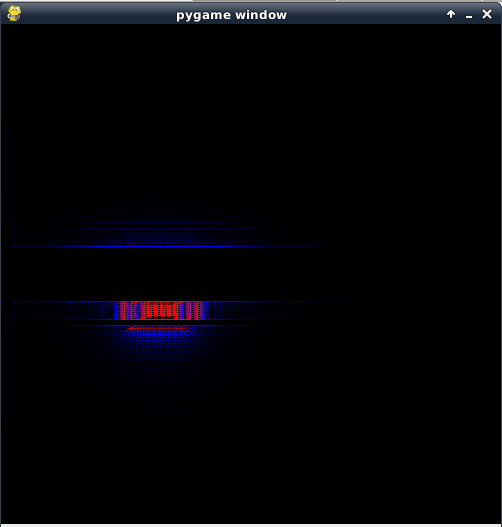
\includegraphics[width=0.3\textwidth]{dc_5} &
		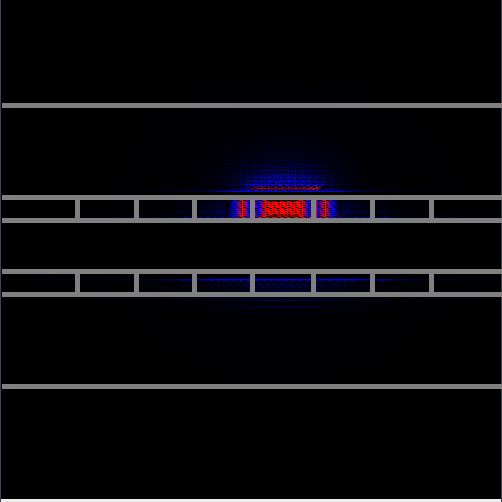
\includegraphics[width=0.3\textwidth]{dc_10} &
		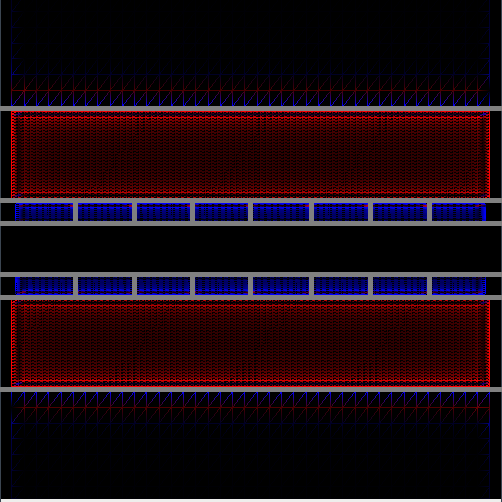
\includegraphics[width=0.3\textwidth]{rf_rails} \\

		
\includegraphics[width=0.3\textwidth]{yz_5} &
		
\includegraphics[width=0.3\textwidth]{yz_10} &
		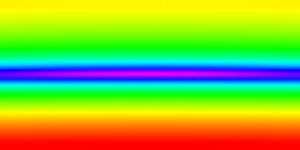
\includegraphics[width=0.3\textwidth]{yz_rf}
	\end{tabular}
	\caption[Electric potentials for sample electrodes in a surface trap]{Electric potential in the center of the Sandia HOA trap caused by charging individual electrodes.  The upper panels show the induced surface charges on the trap electrodes and the lower panels show the electric potential in the vertical and axial directions found using the BEM method.  The left and center panels are for two different dc electrodes, while the right panel shows the pseudopotential resulting from the rf electrode.}
	\label{fig:BEMpots}
\end{figure}

Usually in order to be able to quickly analyze voltage solutions the electric field of each electrode is solved individually (see Figure~\ref{fig:BEMpots}).  Every electrode is set to 0~V except for one which is assigned some nominal value, for example 1~V.  The total electric field for a set of voltages can then be found using superposition by scaling and adding these results for each electrode.  The radial trapping potential is analyzed by performing the same analysis for the rf electrodes and then calculating the electric field from this analysis.  The radial behavior of the ion can be described by an rf pseudopotential approximation
\begin{equation}
	\phi_{\mathrm{pseudo}} = \frac{q}{4 m \Omega_\mathrm{rf}^2}\left| \nabla \vec{E} \right| ^2
\end{equation}
where $\vec{E}$ is the electric field vector, $q$ is the charge of the ion, $m$ is the ion mass, and $\Omega_\mathrm{rf}$ is the frequency of the applied rf voltage.  The secular motion of the ion is described by this potential under the same approximations that we made before, but micromotion is not taken into account.  The minimum of the potential and its harmonic coefficients are found by repeatedly fitting the potential at a trial point to a second order polynomial in three dimensions and moving the trial point along the linear gradient \cite{Blakestad:11}.  When the linear terms are minimized, the bottom of the potential has been found and the harmonic terms can be found by diagonalizing the second order polynomial.

Multidimensional functional minimization is then used to find voltage solutions with desired trap strengths and locations.  Ions can be shuttled axially by solving for voltages that generate a trap every few microns along the region of interest.  Applying these solutions in order at some sufficiently high fixed speed will shuttle the ion at roughly constant velocity.  Stray fields in surface traps can be compensated by finding combinations of voltages that produce electric fields in each direction at the trapping location.  Scaling and combining these electric field generating voltages allows us to cancel any stray field.

Once a trapping potential has been calculated, it must be applied to the dc electrodes.  The current generation of traps have up to 96 dc electrodes that must be independently controlled.  After evaluating potential solutions, including using many 8 channel National Instruments cards in a PCI chassis or a hundred separate high precision DAC chips, we decided to implement a solution using a few many-channel DAC chips.  The AD5372 is an Analog Devices chip that contains 32 independent DACs with 16-bit precision and 20~V output range.  The latter two specifications are sufficient for our needs and, with 32 channels each, three chips suffice to control any of the current generation surface electrode traps.

The disadvantage of using a many-channel chip is that it is not possible to update the voltages of all of the electrodes simultaneously.  Each chip supports a serial interface at 50~MHz and a minimum time between channel updates of 600~ns.  To perform a single step in a shuttling solution it is necessary to update 8 to 10 adjacent electrodes.  These updates must be sent sequentially to separate channels on a single DAC chip which limits the overall update rate to $\approx$ 200~kHz.  The AD5372 does include the functionality to buffer all of the channel updates in a single shuttling step into its registers and then present the voltages simultaneously to the ion trap.  The potential the ion sees is never in an intermediate state and always corresponds to one of the potentials in the solution file even though the updates are communicated serially to the DAC board.

Communication with the DAC chips is accomplished through their serial interface using a custom FPGA software solution implemented on an Altera DE2-115 FPGA development board.  This board features 512~KB of SRAM and a DM9000a ethernet controller.  In order to shuttle the ion, the lab computer loads the shuttling solution from files and transmits it via UDP to the DM9000a ethernet controller.  The FPGA board stores each solution step in SRAM and confirms its receipt to the lab computer.  Once the solution has been loaded it can be played from any desired step to any other at the maximum update rate of the DAC chips by the FPGA.  Since each step could take a different number of channel updates and it is desirable to maintain the same time period between steps in the shuttling solution file the FPGA will automatically generate delays if necessary between solution steps.

Using this system we have successfully trapped barium ions in two different surface electrode traps and have demonstrated shuttling ions.  In order to work on ions at different positions along the axis we have also developed computer controlled systems for positioning the cooling lasers and imaging systems.  We currently shift the position of the cooling lasers using a mirror with a piezoelectric control system.  A custom dc-dc amplifier transforms voltages from an ADC output from a microcontroller into a high voltage input for the piezo mirror.  The microcontroller communicates with the experimental control computer over a serial interface, and it can be program to any desired voltage or to sweep over multiple voltages spending a designated amount of time at each voltage.  This second mode is useful for working on multiple trapping regions at the same time.

In this chapter we have described all of the technology we will need to trap ions for the rest of this work.  Macroscopic linear rf traps are useful for easily evaluating new techniques because of their lower heating rates and easier optical access.  Surface traps will enable us to work with larger numbers of ions and to work efficiently with multiple ion species.  The next two pieces of setup we need are the ionization lasers and the cooling lasers that will create and cool our ions and maintain their low temperatures.  I will discuss these in the next chapter.

\chapter{Working with Barium and Ytterbium}
\renewcommand{\curdir}{ioncool}
\label{sec:ioncool}

\graphicspath{ {\curdir/Graphics/}  }

The two ion species that were chosen to load into these traps as part of our computer architecture were barium and ytterbium.  These elements have several advantages for building a quantum computer using our architecture which will be discussed in this chapter.  Ytterbium will be used to implement the actual quantum computation, while barium will be used to generate remotely entangled ion pairs between ion traps and cool both species.

\section{Ionization}
\label{sec:ionization}

Before any of the trapping technology discussed in the previous section will work we need a source of ions. The atoms to be ionized are generated by heating a small alumina oven tube inside the vacuum chamber.  The oven is loaded with small pieces cut from metallic barium or ytterbium before the chamber is sealed.  It is wrapped with small diameter tungsten wire which is then connected to a vacuum feedthrough.  By running currents between 1-2~A (depending on the length of the wire and its contact with the oven) the oven can be heated to a sufficient temperature to emit a usable flux of the neutral atom.  The flux from the oven is difficult to measure directly, but very reasonable trapping rates of a few ions per minute can be achieved with these currents.  Ionization is accomplished by applying lasers energetic enough to strip the outer electron from the atom, often using intermediate states of the neutral atom to provide isotope selectivity or increase the wavelength of the necessary beams.


\begin{figure}
	\centering
	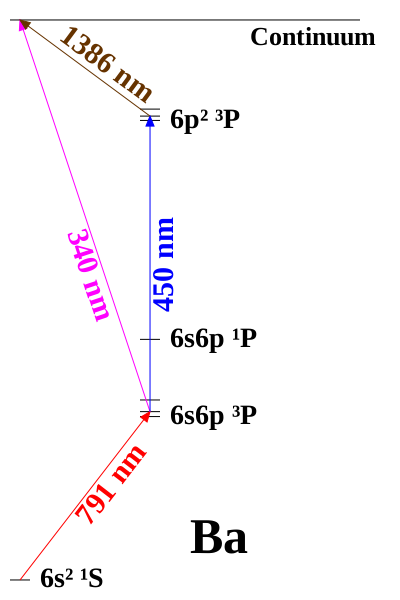
\includegraphics[width=0.5\textwidth]{neutral-Ba}
	\caption[Energy levels of neutral barium]{Energy levels of neutral barium (to scale) \cite{Karlsson:99}.  Possible ionization paths including direct, via 6s6p $^3$P and then direct, and via 6s6p $^3$P and 6p$^2$ $^3$P are shown.}
	\label{fig:neutralba}
\end{figure}

Barium is an alkaline earth metal which makes the atomic structure of its ion easy to analyze.  The spectrum of neutral barium provides many different possibilities for ionization paths as shown in Figure~\ref{fig:neutralba}.  Originally, we directly ionized with a xenon-mercury arc lamp which has ultraviolet spectral components at 237~nm, the ionization threshold of barium.  This method is not isotope selective, and the lamp is generally very difficult to focus.  We then switched to use a two-photon ionization scheme, first driving a transition from the 6s$^2$ $^1$S ground state to a 6s6p $^3$P$_1$ excited state and then ionizing using a 337~nm nitrogen pulse laser.  The first transition, accomplished using a single mode laser diode at approximately 791~nm, provides isotope selectivity.  In addition, both transitions are driven by lasers that can be reasonably well focused near the trapping location.  

The 791~nm laser frequency is stabilized using a side-of-the-fringe locking circuit to a low finesse optical cavity.  This circuit subtracts a constant value from the voltage output of a transimpedance amplifier connected to a photodiode behind the optical cavity.  This voltage provides an error signal that, when fed back to the piezoelectric element in the ECDL with a PID controller, will stabilize the frequency of the laser to a frequency on the side of the cavity line shape.  The cavity itself is temperature stabilized with another PID controller feeding back a temperature signal from a thermistor onto the current through a resistive heater using a MOSFET in the linear regime.  We observe short term frequency stability of a 1-3~MHz and long term drifts of 10-20~MHz, most likely due to residual variation in temperature and changes in atmospheric pressure.

This method of ionization has been very successful for a long time.  The only downside is that it still uses a fairly energetic beam in the 337~nm nitrogen laser.  This laser is energetic enough to easily ionize material deposited on the trap surfaces nearby which can create stray, uncontrolled electric fields that perturb the position of the ion.  This ionization becomes increasingly problematic for wavelengths below 400~nm \cite{Harter:14}.  In macroscopic linear rf traps, this issue has never caused any serious problems because the trap surfaces are several hundred microns from the trapping location and the ionization lasers can be well focused between these surfaces.  When working with surface traps, the trapping region is only separated from the nearest surface by 50-80~microns, and this charging can be a more serious issue.

Therefore, after some initial difficulties trapping in surface traps, we switched to a different ionization scheme that uses only longer wavelength lasers.  The initial step is still the transition driven by the 791~nm laser, but then we instead drive a second intermediate transition to the 6p$^2$ $^3$P$_1$ state using a 450~nm ECDL.  From this excited state the 791~nm or any shorter wavelength laser provides sufficient energy to complete the ionization.  We have successfully used this scheme to ionize barium in surface traps and have not observed excessive charging of the surface during several months of repeated exposure.

\begin{figure}
	\centering
	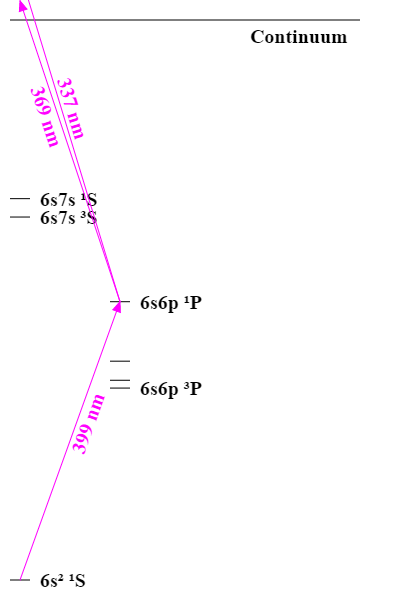
\includegraphics[width=0.5\textwidth]{neutral-Yb}
	\caption[Energy levels of neutral ytterbium]{Energy levels of neutral ytterbiun (to scale) \cite{Sansonetti:05}.  Ionization is achieve using a 399~nm laser and a 369~nm laser.}
	\label{fig:neutralyb}
\end{figure}

Ytterbium is a lanthanoid and has 14 more protons and electrons than barium.  These additional electrons are often bound in the 4f subshell and again, in Yb$^+$ there is a single valence electron in the 6s subshell that is easy to analyze.  There is the additional complication that one of the electrons from the 4f subshell can sometimes be excited to a higher energy subshell giving rise to some additional energy levels with an inner shell vacancy.  Currently we ionize ytterbium using a two-step isotope-selective process.  The neutral atom is addressed with a 399~nm laser that drives a transition from the 6s$^2$ $^1$S ground state to 6s6p $^1$P singlet state which provides isotope selectivity (see Figure~\ref{fig:neutralyb}).  We then ionize using the same nitrogen pulse laser that can be used to ionize barium.  Once we have set up our ytterbium cooling lasers, the 369~nm cooling beam will be a more efficient ionization path from the intermediate state.

\section{Doppler Cooling}
\label{sec:cooling}

When the atoms are ionized they are traveling in a hot thermal beam at a few hundred meters per second, and then suddenly they are affected by the electric fields of the ion trap.  The ions that are trapped need to be cooled to a much lower temperature in order to be well localized so that other operations can be performed on them.  This initial cooling can be accomplished by a technique called laser Doppler cooling.  A strong transition in the ion is addressed by a laser detuned to a frequency slightly lower than the center of the transition.  Cooling is then accomplished using the effect of the Doppler shift because of the ions motion.  When the ion is moving towards the source of the laser, the laser frequency in the ion's rest frame is higher and closer to the center of the resonance.  Therefore the ion absorbs more photons when it is moving towards the laser than when it is moving away from it.  The momentum from these absorptions slows the ion, while the momentum gained from emitting the photons is randomly directed and averages to zero.

The rate at which an ion scatters photons from a laser can be found to be
\begin{equation}
r_{scatter} = \frac{\Gamma}{2} \frac{s}{1 + s + \frac{4 \delta^2}{\Gamma^2}}
\end{equation}
where $\Gamma$ is the linewidth of the atomic transition, $s \equiv \frac{2 \Omega^2}{\Gamma^2}$ is called the saturation parameter, and $\delta$ is the frequency detuning between the source and the center of the atomic transition.  Each photon scattering event also transfers the momentum from the photon to the ions motion.  The resulting force on an ion is
\begin{equation}
	\vec{F}_\mathrm{scatter} = \hbar \vec{k} r_\mathrm{scatter} = \hbar \vec{k} \frac{\Gamma}{2} \frac{s}{1 + s + \frac{4 \delta^2}{\Gamma^2}} \mathrm{.}
\end{equation}
where $\vec{k} = \frac{2 \pi}{\lambda} \hat{k}$ is the photon wavevector.

The Doppler effect modulates this force by causing an additional velocity-dependent frequency shift on the detuning.  The detuning $\delta$ can be rewritten for small ion velocities as $\delta - k v_{ion}$, where $v_{ion}$ is the velocity of the ion with respect to the laser. Cooling can be achieved by choosing these parameters such that the ion experience a force of the form $F = -\gamma v_{ion}$ that acts in opposition to its velocity when $\gamma$ is positive.  For small velocities the force due to photon scattering has the form
\begin{eqnarray}
	F_\mathrm{scatter,doppler} &\approx& F_\mathrm{scatter} - k v_\mathrm{ion} \frac{\partial F_\mathrm{scatter}}{\partial \delta} \\
	&=& F_\mathrm{scatter} \left( 1 + \frac{ 8 k \delta / \Gamma^2 }{ 1 + s + \frac{4 \delta^2}{\Gamma^2} } v_\mathrm{ion} \right)
\end{eqnarray}
where we can identify the term multiplying $v_\mathrm{ion}$ as the damping force coefficient.  For detunings, $\delta$, less than zero this force acts to cool the motion of the ions.

The minimum temperature that can be reached by Doppler cooling is set by the random impulses the ion feels when it emits photons that it has absorbed.  Although these photons are randomly directed and average to no net contribution to the momentum, the ions temperature is still affected by them.  Balancing the cooling rate of the lasers and the heating rate from these random fluctuations, the minimum kinetic energy in the $\hat{x}_i$ direction can be found to be
\begin{equation}
	E_i = \hbar \left( 1 + f_i \frac{r_\mathrm{tot}}{r_\mathrm{i}} \right) \frac{ (\Gamma / 2)^2 + \delta^2 }{8 \delta} \mathrm{,}
	\label{eqn:doppler}
\end{equation}
where $f_i$ is the probability for the ion to scatter a photon in the $\hat{x}_i$ direction and $r_\mathrm{tot}$ and $r_\mathrm{i}$ are the total and fraction due to the beam along the $\hat{x_i}$ direction of the  average scattering rate \cite{Eschner:03, Itano:82}.  We have also assumed that the saturation parameter, $s$, is small.  Figure~\ref{fig:doppler} shows the dependence of the minimum temperature as a function of detuning, $\delta$, for cooling barium ions with a 493~nm laser.  The minimum temperature is $\approx$ 0.25~mK.

\begin{figure}
	\centering
	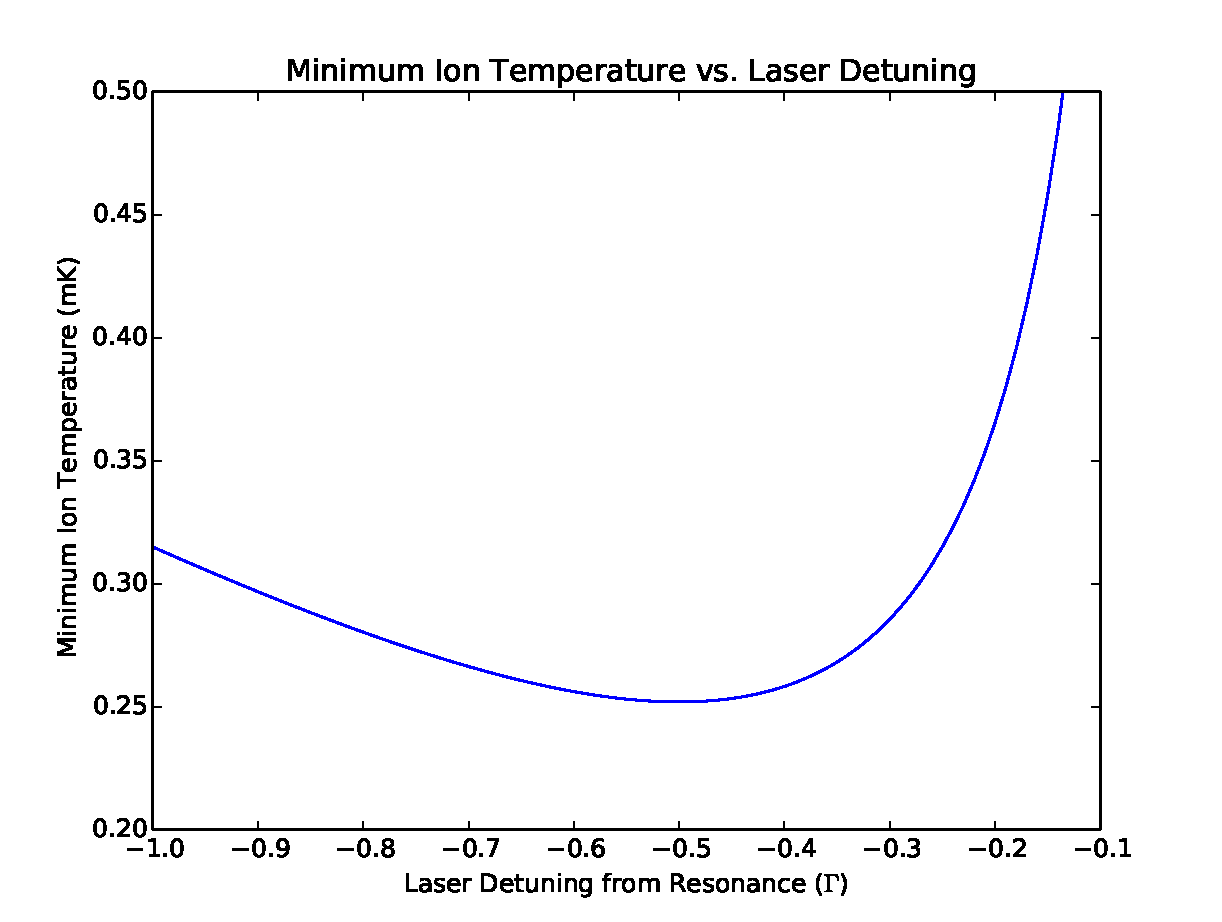
\includegraphics[width=0.8\textwidth]{DopplerCooling}
	\caption[Temperature of Doppler cooled barium ions]{Minimum ion temperature for Doppler cooled barium ions.  The temperature is a function of detuning of the Doppler cooling laser from resonance in units of the natural linewidth $\Gamma$.  The temperature reaches a minimum of $\approx$ 0.25~mK at a detuning of -0.5 $\Gamma$.  Low 493~nm power is assumed and the effect of the 650~nm repump laser is ignored.}
	\label{fig:doppler}
\end{figure}

Doppler cooling barium actually involves using two lasers.  The 493~nm transition scatters the most photons and provides the dominant cooling force.  Unfortunately, there are two possible decay paths from the 6P$_{1/2}$ state that the 493~nm laser excites.  The ion can decay directly back to the 6S$_{1/2}$ ground state from which the 493~nm transition may be driven again to continue cooling, but it may also decay to the long-lived 5D$_{3/2}$ state (see Figure~\ref{fig:ionizedba}).  Since the lifetime of this state is $\approx$ 30~s \cite{Gurell:07} it is necessary to use a second laser to depopulate this state in order to continue to scatter 493~nm photons to cool the ion.  A 650~nm laser is used to drive a transition from the 5D$_{3/2}$ state to the 6P$_{1/2}$ state which closes the cooling cycle because there are no unaddressed decay paths.  This ``repump'' laser complicates the minimum temperature of the ion by introducing an additional laser force as well as two-photon coupling between 6S$_{1/2}$ and 5D$_{3/2}$.  However, when the 650~nm laser is tuned exactly on resonance, the minimum temperature as a function of the 493~nm detuning is only slightly increased.

The 650~nm laser is an external cavity diode laser directly providing approximately 7~mW of optical power, but there were no available 493~nm diodes at the times the setup was designed.  Instead, we have a 986~nm ECDL that produces approximately 150~mW of optical power.  The 986~nm light is sent through an AOM and the first order diffracted beam is sent through a periodically-poled lithium niobate doubling crystal waveguide to produce 493~nm light.  The light can be switched by switching the rf applied to the AOM using a TTL rf switch.  Since this switching is performed in the infrared light, the extinction is squared in the blue light sent to the ion due to the nonlinearity in the frequency doubling process.  We cannot directly measure the actual extinction, but we have determined that it is $>$ 43~dB.  The 650~nm light is shuttered using a single- or double-passed AOM depending on the needs of the experiment being performed (see Figure~\ref{fig:optics}).

\begin{figure}
	\centering
	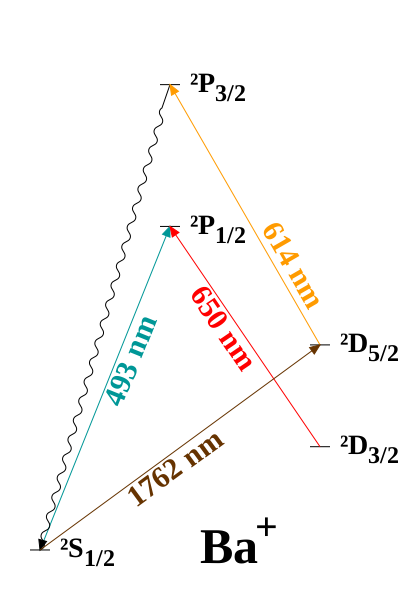
\includegraphics[width=0.5\textwidth]{ionized-Ba}
	\caption[Energy levels of BaII]{Energy levels of singly ionized barium (to scale) \cite{Karlsson:99}.  Laser cooling is accomplished using the 493~nm transition with a 650~nm repump.  The D$_{5/2}$ is used as a ``shelving'' state that is outside of the cooling cycle.  Population can be transferred to D$_{5/2}$ using a 1762~nm laser and returned to the cooling cycle using a 614~nm laser.}
	\label{fig:ionizedba}
\end{figure}

These lasers are already sufficiently stable on short time scales to perform Doppler cooling, but they both exhibit slow frequency drifts on the order of 1~MHz/min that makes it difficult to perform long experiments without stabilization.  For this reason both lasers are stabilized to optical cavities.  The light sent to the optical cavities is offset by an adjustable frequency offset using a DPAOM.  The frequency detuning of the DPAOM is modulated at 20~kHz to modulate the cavity signal.  A phase shifter, frequency mixer, and low pass filter are used to demodulate the cavity signal with the reference 20~kHz modulation signal.  The result is an error signal that crosses zero at the top of the cavity signal.  The error signal is sent through a PID controller and then to a piezoelectric element controlling the feedback frequency inside the ECDL.  As shown in Figure~\ref{fig:optics}, the light being sent to the optical cavity comes from the 0$^{th}$ order of an AOM used for shuttering the light going to the vacuum chamber.  For this reason, the optical power sent to the cavities can vary by a factor of 5 to 10 during an experiment, when the AOMs are frequently turned on and off.  The circuit described here is insensitive to this change in power because it stabilizes the laser to the top of the fringe, whereas the side-of-the-fringe circuit described earlier would cause large frequency shifts whenever the shuttering AOM was switched. 

\begin{figure}
	\centering
	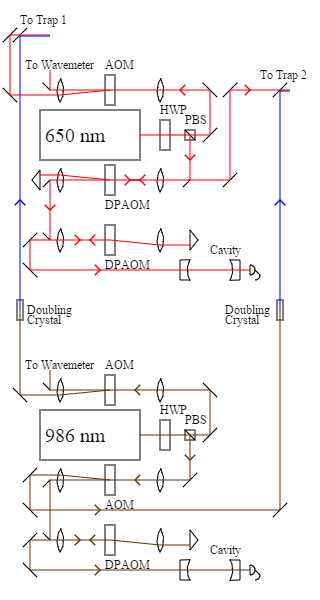
\includegraphics[height=0.6\textheight]{optics-layout}
	\caption[Schematic of optical layout of barium Doppler cooling lasers]{Layout of optics for Doppler cooling barium ions.  A 650~nm ECDL and a 986~nm ECDL are both used. The 986~nm laser is frequency doubled to produce 493~nm light using a nonlinear crystal.  Both lasers are divided into two independent paths to cool ions in two separate vacuum chambers with the amount of power in each beam controllable by a HWP.  The lasers for each trap are then combined using a dichroic mirror and sent to the traps via single mode fiber (not shown).}
	\label{fig:optics}
\end{figure}

A diagram of the Yb$^+$ energy levels is shown in Figure~\ref{fig:ionizedyb}.  The dominant cooling transition is at 369~nm and can be reached using a direct diode.  The $^2$P$_{1/2}$ excited state that is reached via this transition can also decay to a long-lived 5D$_{3/2}$ state.  Unlike in barium, it is most convenient to depopulate this state using a transition to a different excited state formed by exciting an electron from the f shell.  This transition at 935~nm does not introduce any other long-lived possible decay states and the cooling cycle is closed.  There is one other complication in working with ytterbium though.  The ion can be collisionally excited to the 5F$_{7/2}$ state, which has a lifetime of 5.4~years.  We currently do not have any way to repump from this state, which will limit the useful lifetimes of the ytterbium we trap.

The ytterbium lasers are not currently shuttered in any way, although that will be necessary to perform quantum operations on ytterbium ions eventually.  They are again stabilized to optical cavities using a side of the fringe locking circuit similar to the one used with the 791~nm laser.  We are making final preparations to begin using them for cooling the ytterbium ions we have already trapped.

\begin{figure}
	\centering
	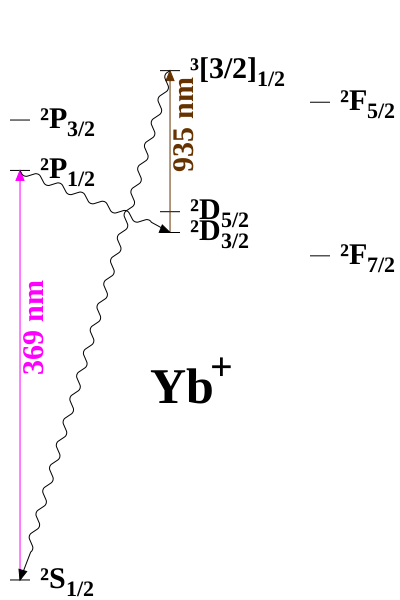
\includegraphics[width=0.5\textwidth]{ionized-Yb}
	\caption[Energy levels of YbII]{Energy levels of singly ionized ytterbium (to scale) \cite{Sansonetti:05}.  Laser cooling is accomplished using the 369~nm transition with a 935~nm repump. The $^2$F$_{7/2}$ state can be collisionally excited and has a lifetime of 5.4~years \cite{Roberts:00}, but can be repumped using a 638~nm laser when this limit to our useful ion lifetime becomes problematic.}
	\label{fig:ionizedyb}
\end{figure}

\section{Initialization and Readout}
\label{sec:initread}

Now we have successfully ionized, trapped, and cooled both barium and ytterbium ions.  In order to begin performing quantum information operations on this system, we need to identify qubits in both that will satisfy the DiVincezo criteria from Subsection~\ref{sec:divincenzo}.  In particular we need to choose two energy states that can be initialized to some simple state representing $\ket{0}$, stay coherent for long enough for our computation to take place, and then be measured.

Ytterbium-171 has some very desirable properties for fulfilling these criteria. It has nuclear spin $\frac{1}{2}$, which means that its 6S$_{1/2}$ ground state is split into two hyperfine levels with $F = 0$ and $F = 1$.  The hyperfine splitting between the two $F$ levels is 12.643~GHZ, and therefore laser line widths are small enough to frequency select which $F$ manifold to address.  The $F = 0$ hyperfine level has only one possible $m_F$ quantum number $m_F = 0$.  The $F = 1$ hyperfine manifold has three levels, $m_F = -1, 0, 1$.  These two $m_F = 0$ levels make excellent qubit levels because they are insensitive to the first order to external magnetic fields.  Coherence times for this qubit of greater than a second have been measured without any kind of magnetic shielding \cite{Olmschenk:07}.  

Initialization and readout of these qubit levels is also very easy.  Readout can be performed by tuning the 369~nm laser to the energy difference between the $F = 1$ manifold in the 6S$_{1/2}$ ground state and the $F = 0$ manifold in the 6P$_{1/2}$ excited state.  Due to angular momentum conservation the decay to the $F = 0$ manifold of the ground state is forbidden.  If the ion was initially in the $F = 1$ qubit level, it will continuously absorb and emit light on this transition until it is off-resonantly driven to the $F = 1$ manifold in the excited state.  Due to the large hyperfine splitting compared to the transition linewidth, thousands of photons can be collected to determine the state with a simple threshold.  Initialization can be performed with a frequency-selective optical pumping scheme.  The 369~nm laser is tuned to the 6S$_{1/2}$ $F = 1$ to 6P$_{1/2}$ $F = 1$ transition because the ion can decay to the unaddressed 6S$_{1/2}$ $F = 0, m_F = 0$ qubit level.  Both of these procedures have been accomplished by applying fixed frequency shifts to the 369~nm laser that can be accomplished by controlling microwaves sent to an EOM for that laser.

Ytterbium-174 has nuclear spin 0 and none of these beneficial properties, but it is more naturally abundant and easier to cool because there are no additional hyperfine levels that need to be addressed to close the cooling cycle.  For this reason, and other experimental limitations we are currently working with Yb-174 instead, but actual quantum computation experiments will use Yb-171 in the future.

Choosing a qubit for operations in barium is somewhat more complicated.  There are three possible isotopes that might be considered for use in quantum computation. Barium-138 is most naturally abundant isotope and it has nuclear spin 0 and therefore no hyperfine structure.  Barium-137 has hyperfine structure because of its nuclear spin I=$\frac{3}{2}$, however this does not give rise to the same nice properties as I=$\frac{1}{2}$.  There are no simple selection rules allowing for easy initialization and detection.  There is an isotope of barium, Ba-133, with nuclear spin I=$\frac{1}{2}$, but it undergoes radioactive decay with a half-life of 10.551~yrs \cite{NuDat}.  Therefore an enriched sample must be used in order to work with this isotope.

Currently we have been working with the easiest isotope, Barium-138. Its ground state is a 6S$_{1/2}$ state with two Zeeman levels $m_J = \pm \frac{1}{2}$.  These levels form a nice qubit, but are very sensitive to magnetic field and maintaining coherence for times longer than $\approx$ 1~ms is quite difficult without magnetic shielding.  Fortunately, following the description of our architecture given earlier, we don't need to store quantum information in this species for long periods of time.  Barium ions can be used to cool the ytterbium ions and to generate remote ion entanglement.  The only time quantum information will be stored in barium is after remote entanglement generation, and this entanglement can easily be transferred to ytterbium ions using a gate sequence of a few hundred microseconds. Since we can work around this short coherence time and the ground state Zeeman levels are otherwise suitable to work with, we have chosen them to be the barium qubit levels in our architecture.  We will still need to be able to initialize and readout these qubit levels in order to perform the remote entanglement and transfer the entanglement to ytterbium ions.

Initialization of these levels is again fairly straightforward.  Circularly polarized light can be utilized to initialize the ion into either Zeeman state.  Because of the conservation of angular momentum, the two circular polarization of light, $\sigma^\pm$, when sent along the quantization axis of the ion, must drive transitions with $\Delta m_J = \pm 1$.  Since the 493~nm transition in ionized barium transfers population between two states with angular momentum $J=\frac{1}{2}$ (see Figure~\ref{fig:ionizedba}), $\sigma^+$ 493~nm light cannot drive a transition from 6S$_{1/2} m_J = +\frac{1}{2}$ to any other state.  However, this light can drive transitions between the 6S$_{1/2}$ $m_J = -\frac{1}{2}$ level and the 6P$_{1/2}$ state. Once the transition is driven, the ion can decay to either ground state Zeeman level.  After the $\sigma^+$ polarized 493~nm light has been applied for a period of time that corresponds to tens of scattering events ($\approx$ 100 $\mu$s), population will accumulate in the $m_J=+\frac{1}{2}$ level because no lasers are addressing this level.

In other trapping systems we have implemented this procedure using two separate 493~nm beams.  One beam is focused onto the ion along the quantization axis with linear polarization and therefore can drive transitions from either Zeeman level and will Doppler cool the ion.  The other beam is sent along the quantization axis with a circular polarization to perform optical pumping.  By shuttering the linearly polarized beam, the ion can be optically pumped to the state the circularly polarized beam does not address.

Since our setup switches the 986~nm beam before it is frequency doubled (see Figure~\ref{fig:optics}) the optical pumping procedure can not be implemented in the same way because we cannot independently shutter two 493~nm beams well.  Instead, a single 493~nm beam is sent to the trap.  The beam passes through a quarter wave plate which initializes it to a circular polarization and then through a Pockels cell.  The Pockels cell is oriented so that when charged to 1.1~kV the 493~nm beam can be rotated back towards linear polarization.  Therefore the 493~nm beam can be switched from performing Doppler cooling to performing optical pumping as quickly as the voltage can be switched in the Pockels cell.  We use a modified piezeoelectric actuator driver circuit to implement this switching in $<$ 2~ms based on a TTL signal.

In order to readout the Zeeman levels of the barium ions we cannot play a simple trick as in ytterbium.  Unfortunately, there are no selection rules to prevent decays from the excited state to either of our qubit states.  Instead we have to transfer the population from one of the qubit states to a long-lived state outside of the cooling cycle.  In Figure~\ref{fig:ionizedba}, we can see that there is such a state, the 5D$_{5/2}$ state.  The 5D$_{5/2}$ state has a lifetime of 30~s, which is more than sufficient since we can determine whether the ion is in the cooling cycle by monitoring its fluorescence for $<$ 20~ms.

Population can be transferred to the \ba 5D$_{5/2}$ using a narrow, 1762~nm fiber laser.  This laser produces $\approx 5~mW$ of optical power with a linewidth of $\approx 100~Hz$ \cite{Noel:12}.  It is locked to a temperature and pressure stabilized Zerodur optical cavity with a linewidth of 500~kHz \cite{Dietrich:10} with about half of the laser power.  With the power remaining after frequency stabilization, coherent $\pi$-pulses from the 6S$_{1/2}$ ground state to the 5D$_{5/2}$ excited state can be achieved in as short as 10~us.  Since the natural linewidth of the transition and the Rabi frequency with which we drive it are both much smaller than the separation between the two Zeeman levels we can frequency select which Zeeman level we are addressing.  The laser is shuttered by a single pass AOM with a frequency bandwidth of $\approx$ 10~MHz that will also be used to perform frequency scans.

Using this laser readout of the Zeeman state of the \ba ion is achieved by transferring or ``shelving'' one of the Zeeman states to the 5D$_{5/2}$ level.  The cooling lasers are then applied for 20~ms and a simple threshold is used to separate background PMT counts from the counts of a fluorescing ion.  The ion will only be fluorescing if the valence electron was initially in the unshelved Zeeman state.  Once this determination has been made, if the electron was successfully shelved it can be brought back into the cooling cycle without having to wait for the $\approx 30~s$ lifetime by applying light at 614~nm (see Figure~\ref{fig:ionizedba}).

The tools we have developed for manipulating the ground state Zeeman levels of barium will enable us to begin investigating the feasibility of a mixed species ion trap quantum computer.  In Chapter~\ref{sec:modes}, we will analyze the motional modes of these chains and measure their temperatures and heating rates.  In the near future, we will be finishing our development of the infrastructure for working with ytterbium ions.





\part{Measurements in Surface Traps and Mixed Species Ion Chains}

\chapter{Surface Traps}
\renewcommand{\curdir}{surface}
\label{sec:surface-meas}

\graphicspath{ {\curdir/Graphics/}  }

Surface electrode traps have several advantages over standard ``macro'' ion traps.  They can be repeatably manufactured and provide a large number of independent dc voltage parameters that can be used to precisely control the location and motion of trapped ions.  The difficulty in working with these traps is the decreased distance between the ions and the nearest surface.  Material deposited on these surfaces during the vacuum bake out or from the ovens can be charged and induce stray fields and additional heating on the ions.  Characterizing both of these problems is important for being able to perform high fidelity work in these systems.  We have performed some initial characterization of surface traps that we have been working with.  

\section{Ion Dark Lifetime}
\label{sec:lifetime}

One of the initial difficulties with working with surface traps was their poor ion lifetimes.  Even while being cooled ions would only stay trapped for minutes, and, without continuous cooling, lifetimes were often as small as a few seconds.  The first trap that we performed measurements in was a Sandia National Labs ``Y'' trap.  This surface electrode trap has three arms extending radially from a central point where they are all connected.  The radial trap is formed by rf and dc rails that run along the side of each arm.  Near the end of each arm there is a 100~micron by 100~micron hole through the entire chip that allows neutral atom flux to travel from behind the trap to be loaded into the trapping region above it.

Cooled lifetimes in this trap were easily tens of minutes, and further investigation of them would have been painfully slow so we performed measurements of the dark, uncooled lifetime instead.  An automated loading procedure was developed leveraging our TTL control over all ionization lasers and our neutral atom oven.  This system allowed the entire experiment to be automated even though it involved losing and retrapping ions many times.

Measuring dark lifetimes itself is straightforward.  A single ion is trapped and cooled using our normal cooling apparatus.  The cooling lasers are then well shuttered for a fixed period of time during which the ion is expected to heat.  The cooling lasers are then unshuttered and fluorescence is collected to determine if the ion remained in the trap.  If it did not, another ion is trapped, and then the experiment is repeated.

This measurement is expected to give some insight into the heating rate of ions in the trap.  The heating rate of ion traps is complicated but is related to the stray field and electric field noise environments of the ion.  Using our shuttling system we were able to repeat the measurement at different location along one arm of the trap.  It was expected that because of the neutral atom flux deposited underneath the loading hole this region could develop a large stray vertical electric field which would increase heating in this region.  

Motional heating in ion traps is a complicated phenomenon and is only recently beginning to be investigated systematically.  There are a number of phenomena known to cause heating including rf electric field noise near trap junctions, DAC sampling noise, and electric field noise at the secular frequencies \cite{Blakestad:09, Blakestad:11}.  The first heating source is significant in junctions in surface traps because there may be significant gradients in the rf pseudopotential.  The update rate of the DACs has strong frequency components that can cause direct heating of motional modes or combinations of motional modes through parametric resonances.

\begin{figure}
	\centering
	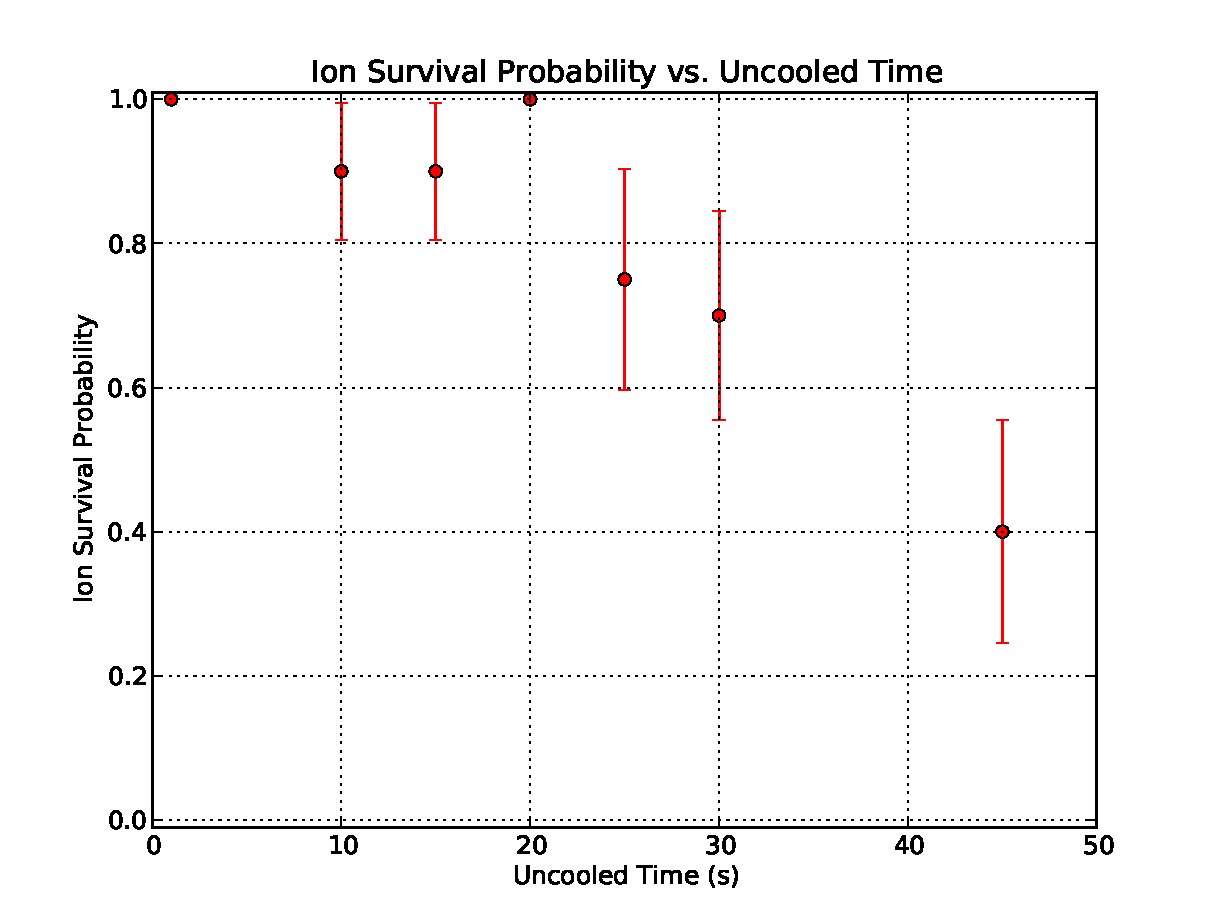
\includegraphics[width=0.7\textwidth]{LifetimeLoadingHole}
	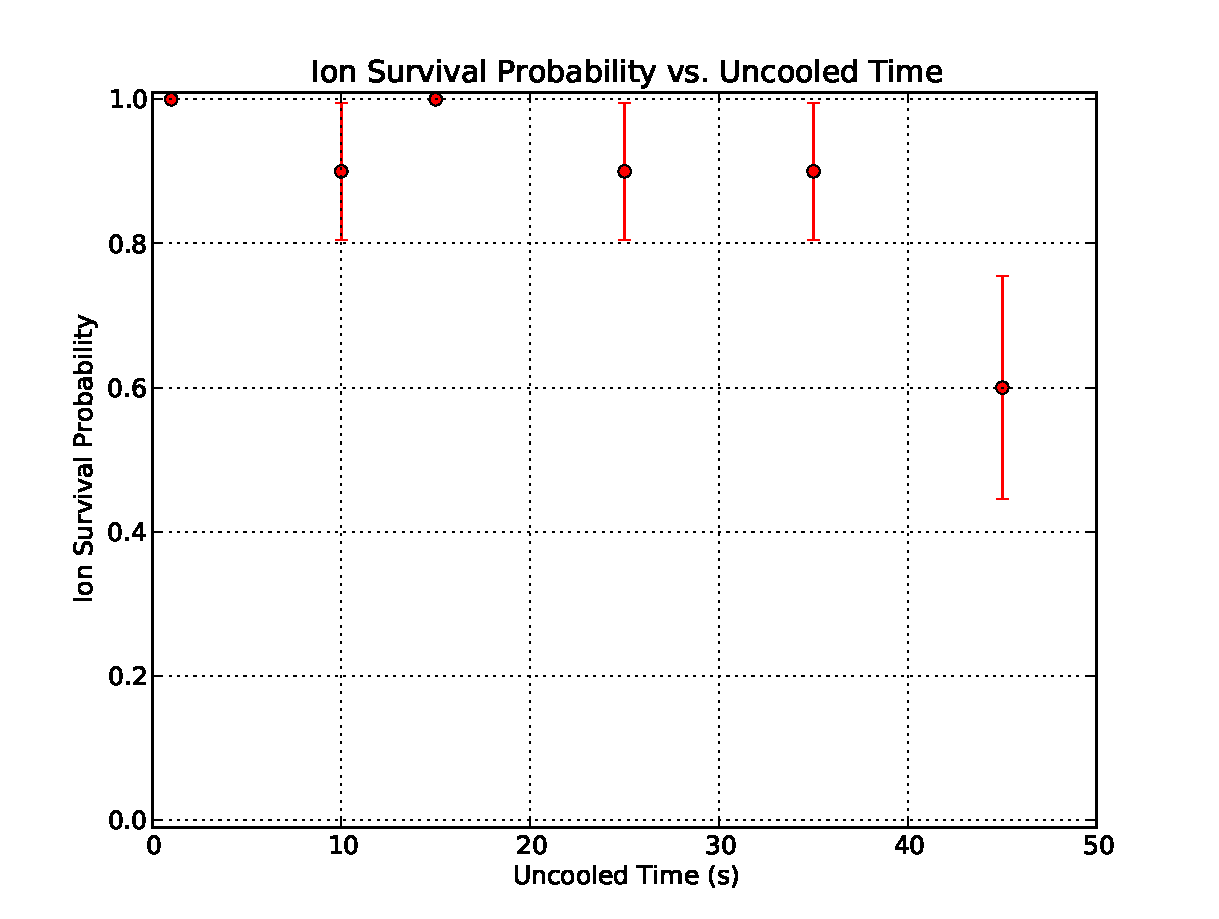
\includegraphics[width=0.7\textwidth]{LifetimeMidarm}
	\caption[Dark lifetime of barium ions in Sandia Y trap]{Dark lifetime of barium ions in a Sandia ``Y'' trap.  The probability that an ion remains trapped and can be recooled after a period of time without Doppler cooling.  This lifetime is significantly shorter in the loading region of the trap (top) than several hundred microns away along the trap (bottom).}
	\label{fig:lifetime}
\end{figure}

Direct heating from electric field noise at the motional secular frequencies has historically been anomalously high.  Heating rates seem to strongly increase as ions are brought closer to surfaces in ion traps, which has made the problem increasingly troublesome as the community moves towards using surface traps where ions are located 40~um to 100~um from the surface of the trap.  The expected scaling for the heating rate as a function of the distance to the nearest surface, $d$, would be $d^{-2}$, but instead there is significant evidence that the dependence is $d^{-4}$.  This problem has often been addressed in the past by using cryogenic instead of room temperature ion trap systems which greatly reduces the electric field noise density \cite{Niedermayr:14, Labaziewicz:08, Chiaverini:14}.  Recent investigations have shown that this surface heating is probably due to electric field noise in contaminants deposited on the surface during the UHV bakeout \cite{Safavi:11,Hite:12}.  These contaminants can be removed by argon ion bombardment after bakeout, which in two separate studies significantly lowered the heating rate in the trap \cite{Hite:12,Daniilidis:14}.

While we are beginning to develop an understanding of the processes behind this heating rate, at the moment it is still one of the most difficult experimental problems in surface traps.  In trapping systems that were not designed to be cleaned by ion bombardment, characterizing and dealing with the trap heating rate is important.

From Figure~\ref{fig:lifetime}, it is clear from our results that there is additional heating near the loading region.  It is beneficial to have regions of the surface trap that do not have loading holes where the heating rates may be lower and quantum operations can be performed more easily.  An additional benefit is that ions can be loaded while quantum operations are being performed without the neutral atom flux perturbing the calculation.  

\section{Secular Frequencies and Stray Fields}
\label{sec:secfreqs}

As discussed in Section~\ref{sec:paul}, the ions' motion can be approximately described as the result of a harmonic potential in each direction.  Measuring the trap frequencies in each direction allows us to characterize the strength of the trapping potential.  A technique to measure these frequencies is to apply a small-amplitude, oscillating electric field and scan its frequency over the possible range for the ions secular frequency.  We can understand the response of the ion to this ``tickle'' voltage by approximating its equation of motion as
\begin{equation}
	\ddot{x} + \omega_x^2 x = \frac{q \vec{E}_t \cdot \hat{x}}{m} \cos( \omega_t x )
\end{equation}
where $\omega_x$ is the radial secular frequency, $q$ is the charge of the ion, $\vec{E}_t$ is the magnitude and polarization of the tickle field, and its angular frequency is $\omega_t$.  This driven harmonic oscillator equation exhibits large amplitude motion when $\omega_t$ is approximately a multiple of $\omega_x$.

Another method for applying the ``tickle'' amplitude is to apply an additional high frequency voltage to the rf electrodes inside the trap.  When this signal's frequency, $\omega_t$, is offset from the applied rf frequency by a multiple of one of the trap frequencies, large amplitude motion can again be observed.  The tickle signal is added to the normal trapping rf using an rf splitter/combiner before the signal is amplified.  Although the rf then passes through a resonator with a Q factor of $\approx$ 200 which acts as a narrow-band filter, enough of the tickle signal remains for the additional motion to be detected.  The advantage of applying the signal this way is that the amplitude of the motional signal the ion sees is minimized when the stray electric field has been compensated, as discussed below. 

The motion of ions in a linear rf trap is given by Equation~\ref{eqn:mathieu-soln} if there is no stray electric field at the trapping location.  Additional micromotion caused by a stray field, $\vec{E}$, adds a term $B_x = q \vec{E} \cdot \hat{x} / m \omega_x^2$ to the solution of the Mathieu equation.  The radial motion of the ions is described by
\begin{equation}
	x(t) = \left( B_x + A_x \cos( \omega_x t + \phi_x ) \right) \left( 1 + \frac{q_x}{2} \cos( \Omega_\mathrm{rf} t ) \right) \mathrm{,}
\end{equation}
where $\Omega_\mathrm{rf}$ is the frequency of the applied rf, $q_x$ is a parameter of the Mathieu equation, and $A_x$ and $\phi_x$ are an amplitude and a phase set by initial conditions.  The larger the motion of the ion at $\Omega_\mathrm{rf}$ due to stray fields, the stronger the Doppler modulated signal from the tickle field it will see at $\omega_t - \Omega_\mathrm{rf}$.  By applying the tickle voltage at $\Omega_\mathrm{rf} + \omega_x$ and minimizing the ions response to it, the micromotion in all three axes can be minimized \cite{Ibaraki:11,Mount:13}.  

The additional motion of the ion caused by either of these tickle voltages can be detected by observing the image of the ion on a CCD camera.  On resonance the amplitude of the ions' motion can increase to $\approx$ 10~$\mu$m distance scales that are easily resolvable.  Since the motion of the ion is much faster than the exposure time of the camera, the ion's image appears to blur out over a larger area while it is being heated and collapse to a small point when cold.  The direction of this blurring can be seen in the CCD images and used to identify the trap axis that is being excited.  Figure~\ref{fig:tickle} shows the ions' response to being driven with an rf tickle near its axial trap frequency.  The additional heating can also be detected by detuning the Doppler cooling laser several linewidths from the transition so that normally the fluorescence is very low.  When the ion is heated it occupies much higher motional states and additional fluorescence can be seen \cite{Mount:13}.

\begin{figure}
	\centering
\begin{tabular*}{0.6\textwidth}{cccc}
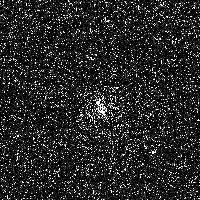
\includegraphics[width=0.1\textwidth]{axial/crop171} &
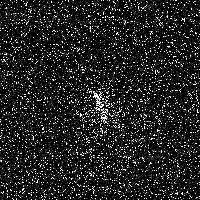
\includegraphics[width=0.1\textwidth]{axial/crop173} &
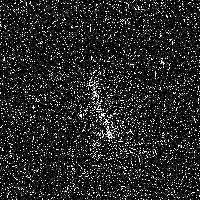
\includegraphics[width=0.1\textwidth]{axial/crop176} &
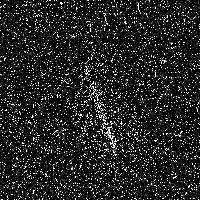
\includegraphics[width=0.1\textwidth]{axial/crop178} \\
{\small 24.171 MHz} & {\small 24.173 MHz} & {\small 24.176 MHz} & {\small 24.178 MHz} \\[0.5in]
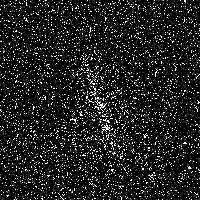
\includegraphics[width=0.1\textwidth]{axial/crop181} &
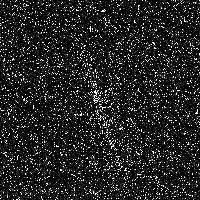
\includegraphics[width=0.1\textwidth]{axial/crop183} &
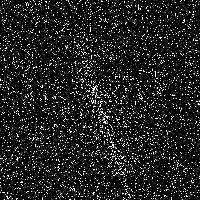
\includegraphics[width=0.1\textwidth]{axial/crop185} &
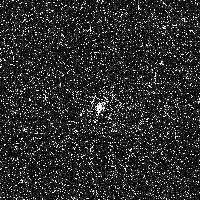
\includegraphics[width=0.1\textwidth]{axial/crop187} \\
{\small 24.181 MHz} & {\small 24.183 MHz} & {\small 24.185 MHz} & {\small 24.187 MHz} \\ 
\end{tabular*}
	\caption[CCD images of a barium ion with resonant rf modulation]{CCD images of a single \ba ion at different applied rf tickle frequency indicated underneath each image. The trap rf frequency, $\Omega_\mathrm{rf}$, was 24.93~MHz.  The amplitude of the ions motion increases dramatically when the tickle frequency is offset from the carrier frequency by a multiple of the trap frequencies.  The excitation shown is the trap axial mode which in these images is oriented along an axis approximately 30 degrees counter-clockwise  from vertical.}
	\label{fig:tickle}
\end{figure}

Using this measurement technique we have measured the secular frequencies of our trap with the voltages we are currently applying.  The axial angular frequency is $\approx$ 2$\pi \times$ 0.75~MHz using dc voltages of order $\pm$ 5~V, and the radial frequencies are $\approx$ 2$\pi \times$ 1.50~MHz and 2$\pi \times$ 2.05~MHz with approximately 100~Vpp of 20~MHz rf.  



\chapter{Normal Modes in Mixed Species Ion Chains}
\renewcommand{\curdir}{modes}
\label{sec:modes}

\graphicspath{ {\curdir/Graphics/}  }

The motional states of trapped ions are shared between all ions in the trap and provide a mechanism for transferring information between these ions.  By applying detuned lasers, virtual phonons can be excited and absorbed in motional modes shared by two or more ions, and the entangling M\o{}lmer-S\o{}rensen gate can be implemented.  In order for this to work the modes must be kept relatively cold, using Doppler cooling or other techniques.  For chains that include mixed ion species, the normal modes can separate, with some modes only coupling to one ion species and some to the other.  This effect limits our ability to cool both ion species using only cooling lasers addressing one species.  We have begun investigating the ion temperatures and heating rates in mixed species chains.  For the moment, we are performing these measurements in a standard macroscopic linear rf trap, but we plan to begin using them to characterize different surface trap designs in the near future.

\section{Single Ion Normal Modes}
\label{sec:single-modes}

In the case of a single ion occupying a trapping region there are only three normal modes.  At the bottom of the trap, the ion sees a harmonic potential in each direction and its motional states are well described by quantum harmonic oscillator states.  We will begin by only considering one mode of motion in the $\hat{x}$ direction.  We can label the motional states by $\ket{0}$, $\ket{1}$, etc. with energy $E_n = \hbar \omega (n + \frac{1}{2})$.  We can also define raising and lowering operators $a$ and $a^\dagger$ and write the position of the ion in terms of them as $x = x_0 (a + a^\dagger)$ where $x_0 = \sqrt{\frac{\hbar}{2 m \omega_x}}$ and $m$ is the mass of the ion.  After Doppler cooling the ion is in a thermal mixed state of these motional levels.  The density matrix of the ion is described by a parameter $\bar{n}$, the average thermal motional occupation number, and can be written
\begin{equation}
	\rho = \sum\limits_{n=0}^{\infty} \frac{1}{\bar{n}+1} \left( \frac{\bar{n}}{\bar{n} + 1} \right) ^ n \ket{n} \bra{n} \mathrm{.}
\end{equation}

In order to analyze the temperature of the motional modes we first took some measurements with a single ion.  In particular, we measured $\bar{n}$ and its time derivative $\dot{\bar{n}}$ to determine these parameters in the linear rf trap where we will later perform mixed ion species experiments.  The initial average thermal motional occupation number, $\bar{n}$, provides information on how effective Doppler cooling is, and can be indicative of problems with the cooling laser powers and frequencies.  The parameter $\dot{\bar{n}}$ is often called the heating rate, and is likely to be roughly constant as more ions are added.  Heating rates in macroscopic traps are often less problematic than in surface traps because of the increased distance between the nearest surfaces and the trapping locations, but the techniques we develop can later be used when these experiments are moved to surface traps.  

In order to make measurements of these parameters of the normal modes of the ion trap, we have to understand the way electric fields can interact with the modes.  In particular, we will be driving sideband transitions using lasers addressing narrow optical transitions.  Consider an atomic system consisting of two qubit levels $\ket{\downarrow}$ and $\ket{\uparrow}$, as well as harmonic motional energy levels in the $\hat{x}$ direction with angular frequency $\omega_x$.  Our base Hamiltonian is then
\begin{equation}
	H = \hbar \omega_\downarrow \ket{\downarrow}\bra{\downarrow} + \hbar \omega_\uparrow \ket{\uparrow}\bra{\uparrow} + \hbar \omega_x a^\dagger a \mathrm{,}
\end{equation}
where $\hbar \omega_\downarrow$ and $\hbar \omega_\downarrow$ are the energies of the two qubit levels.  We will consider the interaction of this ion with monochromatic electromagnetic radiation described by the potential energy
\begin{equation}
	V = \hbar \Omega \left( \ket{\uparrow}\bra{\downarrow} + \ket{\downarrow} \bra{\uparrow} \right) \left( e^{i k_x x + i \omega t} + h.c. \right) \mathrm{,}
\end{equation}
where $k_x$ is the component of the photon wavevector in the $\hat{x}$ direction, $\omega$ is the angular frequency of the radiation, $\Omega \equiv \frac{\vec{\mu} \cdot \vec{E}}{\hbar}$ is the Rabi frequency of the transition defined as in Chapter~\ref{sec:qcomp} in terms of the electric field magnitude and polarization, $\vec{E}$, and the ion dipole moment, $\vec{\mu}$.  Transforming the Hamiltonian into the interaction picture, we find
\begin{equation}
	V_I(t) = \hbar \Omega \left( \ket{\uparrow}\bra{\downarrow} \exp \left( i \eta (a e^{-i \omega_x t} + a^\dagger e^{i \omega_x t}) + i (\omega - \omega_{\uparrow} + \omega{\downarrow}) t \right) + h.c. \right) \mathrm{,}
\end{equation}
where $\eta \equiv x_0 k_x$ is the Lamb-Dicke parameter defined in Chapter~\ref{sec:qcomp}.  The effect of the ion's motion on the optical transitions between motional states $n$ and $n'$ can be absorbed into $\Omega$ and $\delta$ by writing
\begin{eqnarray}
	\Omega_{n,n'} &=& \Omega \left| \bra{n'} \exp\left( i \eta (a + a^\dagger ) \right) \ket{n} \right| \\
	&=& \Omega e^{-\eta^2 / 2} \left( \frac{n_<!}{n_>!} \right)^{1/2} \eta^{\left| n - n' \right| } L_{n_<}^{\left| n - n' \right| }(\eta^2) \\
	\delta_{n,n'} &=& \omega - \omega_\uparrow + \omega_\downarrow - \omega_x (n' - n)
\end{eqnarray}
using the generalized Laguerre polynomials, $L_n^\alpha$, and defining the smaller of $n$ and $n'$ to be $n_<$ and the larger to be $n_>$.  The transition between $\ket{\uparrow}$ and $\ket{\downarrow}$ proceeds as in Chapter~\ref{sec:qcomp}, but with additional transitions corresponding to any choice of $n$ and $n'$ occurring with the corresponding $\Omega_{n,n'}$ and $\delta_{n,n'}$.

Therefore, we can see that we can drive transitions between motional states of the ion using an optical electric field.  In order to observe these sideband transitions in trapped barium ions, we use the techniques discussed in Section~\ref{sec:initread}.  We trap and Doppler cool a single \ba ion, and then initialize its state to the $m_J$ = -1/2 level of its 6S$_{1/2}$ ground state by switching our cooling laser to have circular polarization.  We then shutter the cooling lasers and apply a fixed duration pulse of 1762~nm light that is near the transition from the optically pumped ground state to the $m_J$ = -1/2 level of the 5D$_{5/2}$ state.  Upon reactivating the cooling lasers we see fluorescence from the ion only if we were unsuccessful in driving a transition with 1762~nm laser.  This procedure is repeated multiple times to build statistics, and then repeated at multiple frequencies of the 1762~nm laser to explore the frequency dependence of the transition. 

Figure~\ref{fig:freqscan} shows the result of this procedure.  The large center peak is the carrier transition ($n'$ = $n$) that does not include any change in motional state.  There are two sets of red ($n'$ = $n-1$) and blue ($n'$ = $n+1$) sidebands of this transition visible corresponding to the two radial motional modes.  The strength of the sidebands is related to the carrier transition by $\eta \sqrt{\bar{n}}$ and therefore depends on the photon momentum, the motional secular frequency, and the occupation number.  The two sidebands that are shown are the radial sidebands with secular frequencies of $\omega_x$ = $2 \pi \times$ 1.31~MHz and $\omega_y$ = $2 \pi \times$ 1.21~MHz.  The 1762~nm laser is oriented perpendicular to the trap axis and therefore no axial sideband transition can be seen because the corresponding $\eta = 0$.

\begin{figure}
	\centering
	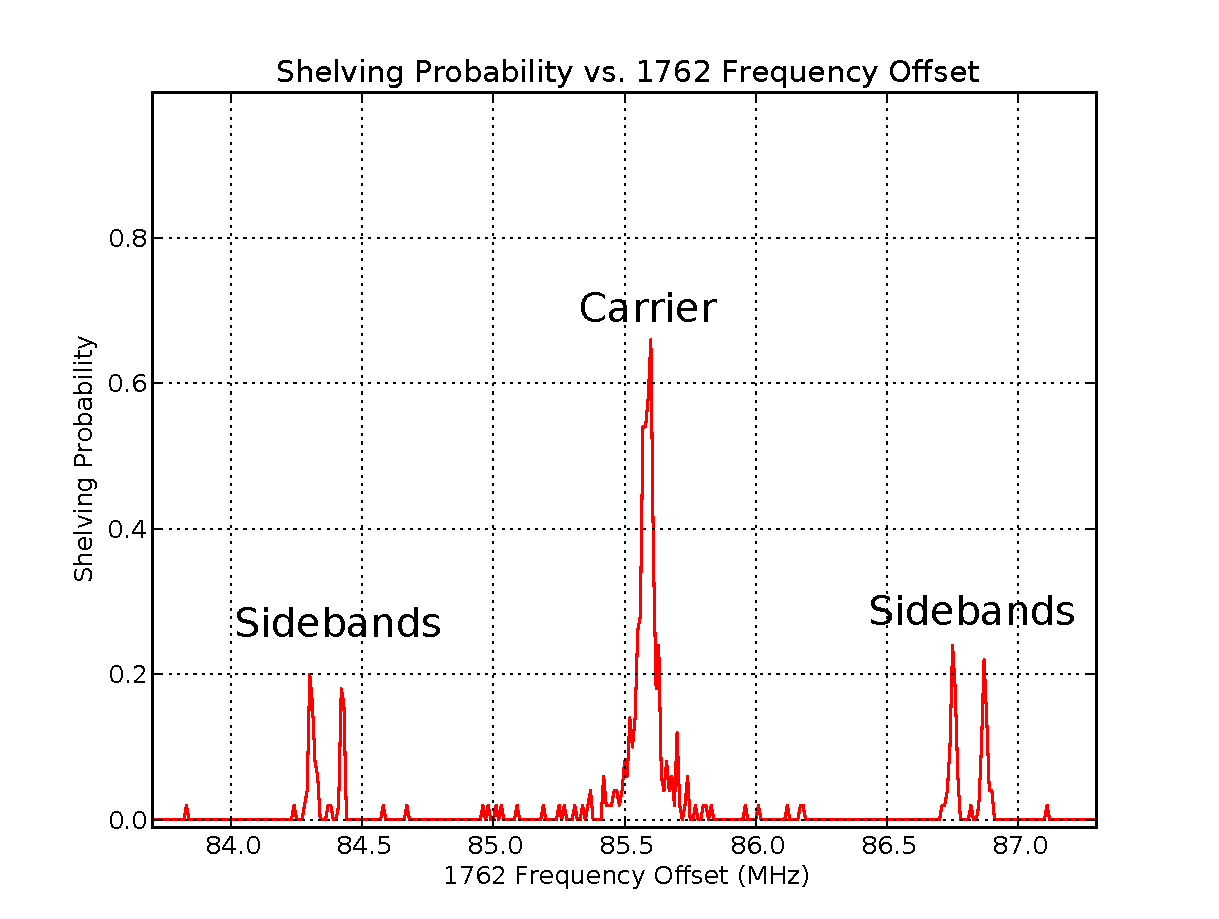
\includegraphics[width=0.8\textwidth]{FullScan}
\caption[Motional mode spectroscopy of the 1762~nm transition in \ba]{Motional mode spectroscopy of the 1762~nm transition in \ba.  Shelving probability is shown as a function of 1762~nm laser frequency.  A strong carrier transition is present at offset 85.6~MHz, while symmetric radial motional sidebands can be seen at 84.3~MHz, 84.4~MHz, 86.75~MHz, and 86.85~MHz.}
	\label{fig:freqscan}
\end{figure}

Using this technology we would then like to estimate the initial temperature and heating rate of our ions.  There are two possible methods for performing this procedure.  We could compare the strength of the sidebands to the strength of the carrier and use the weak excitation limit from Equation~\ref{eqn:shortpulses} to extract $\eta \sqrt{\bar{n}}$ for each peak.  The difficulty with this strategy is that the radial modes must be weakly excited in order to extract this information, and errors on fitting the heights of the peaks are often large.  For single ions we can make a more accurate measurement by using a different technique based on measuring the decay of contrast in carrier Rabi oscillations.

Since our 1762~nm source has a linewidth $<$ 1~kHz we should be able to apply pulses of hundreds of microseconds of duration without seeing any noticeable loss of contrast in Rabi oscillations.  Instead the amplitude of these oscillations begins to decay in 100~$\mu$s to 200~$\mu$s because of the finite temperature of our ions.  The source of this loss of contrast is driving carrier (not sideband) transitions from different motional harmonic oscillator states.  The sideband transitions are far enough away in frequency that they are not relevant, but these carrier transitions at different motional energies are slightly shifted in frequency with respect to one another.  All of these transitions of slightly different frequency are driven simultaneously and the accumulating phase difference between them causes a decrease in contrast.

The Rabi frequency for these carrier transitions follows from the above discussion of sideband transitions and is
\begin{equation}
	\Omega_{n,n} = \Omega e^{-\eta^2/2} L_n^0 ( \eta^2 ) \mathrm{,}
\end{equation}
which can be simplified for $\eta^2 \ll 1$ to $\Omega ( 1 - \eta^2 n )$.  In order to calculate the result for an ion at a finite temperature we can write the probability of driving the transition as a sum over a thermal distribution of motional states. The probability of driving the transition to the shelved state becomes
\begin{equation}
P_\mathrm{shelve} (t) = \sum\limits_{n=0}^{\infty} \frac{1}{\bar{n} + 1} \left( \frac{\bar{n}}{\bar{n} + 1} \right) ^n \sin^2 \left( \Omega_{n,n}  \frac{t}{2} \right) 
\end{equation}
This analysis has all been performed assuming there is only one motional degree of freedom.  If the ion has multiple modes of motion there is a corresponding Lamb-Dicke parameter, $\eta$, and thermal average occupation number, $\bar{n}$, for each mode.  The shelving probability can be calculated by summing over all possible combinations of occupation numbers in each mode weighted by the thermal state probability for each mode.  For even a few modes this calculation becomes very time consuming, and the fit parameters are coupled together which decreases the accuracy of the fit.  The computational time can be reduced by Monte Carlo sampling from the distribution of occupation numbers, but the errors would still be large.

Instead we have chosen the propagation angle of the 1762~nm laser to only address the radial modes of motion, which are separated in frequency by $\le$ 10\%.  It is therefore reasonable to approximate their occupation numbers and Lamb-Dicke parameters as equal.  Since the axial trap frequency is almost an order of magnitude smaller this procedure would not be possible if the 1762~nm laser also addressed these states.  Making this approximation for the radial parameters, we can extract a parameter $\sum_i \bar{n}_i$, where the sum extends over two radial modes, from an experimental Rabi flop curve.

Using this procedure, we would like to find the minimum temperature we achieve with Doppler cooling, as well as the rate at which the ion heats while Doppler cooling is disabled.  In order to find this heating rate, we can shutter the cooling lasers for a variable period of time before applying 1762~nm pulses to it.  In Figure~\ref{fig:rabi-heating} we can see that as we increase the period of time that the cooling lasers are shuttered the Rabi oscillations lose contrast more rapidly which corresponds to an increase in temperature of the ion.  It is common to approximate the heating rate in ion traps as linear, and this approximation holds well at least for low temperatures.  As the ion heats up and experiences more of the trap anharmonicity and trap micromotion, heating rates may increase, but we do not see evidence of this at the temperatures we currently reach.  The total initial radial mode average occupation of our single trapped barium ion is 122~quanta for two modes, with a total heating rate of 2.43~quanta/ms (see Figure~\ref{fig:heating-nonoise}).

\begin{figure}
	\centering
	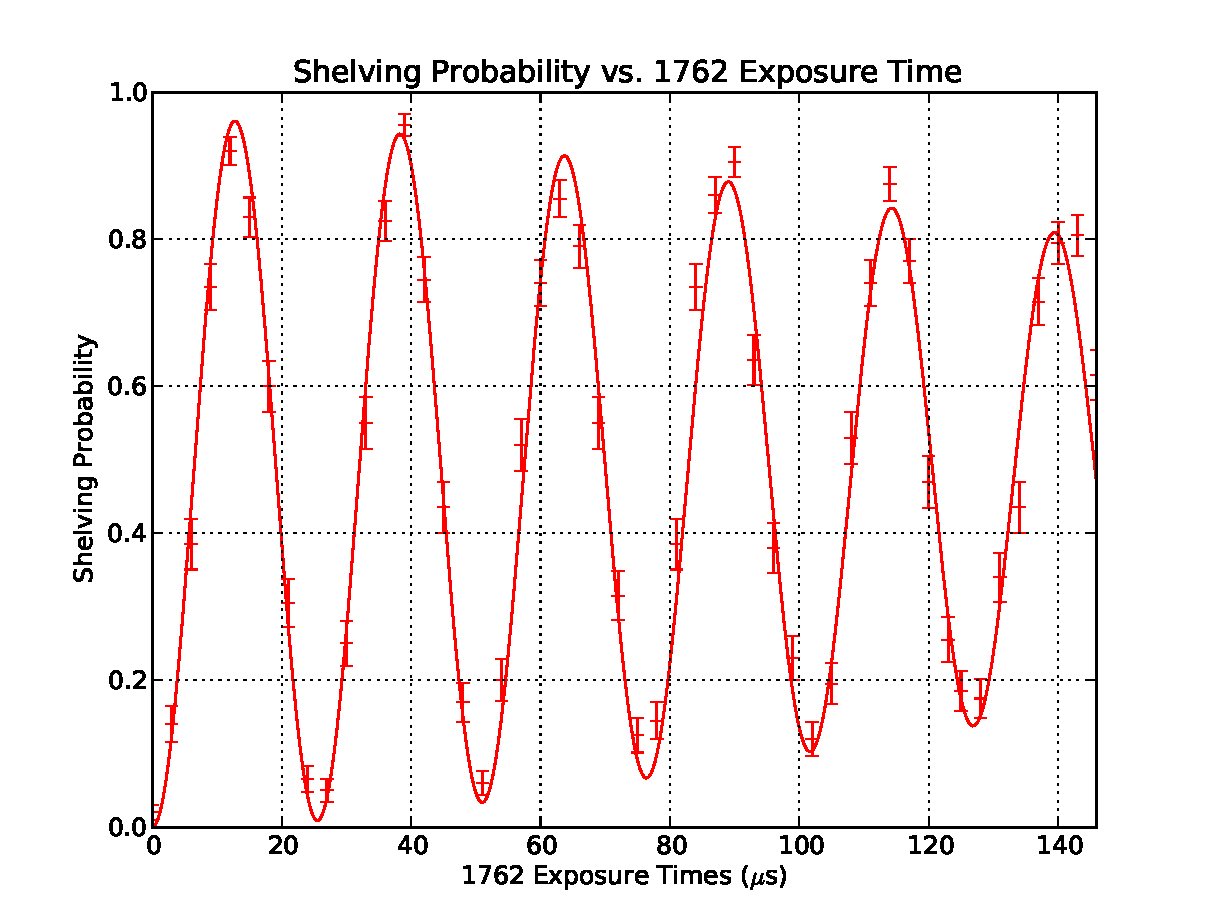
\includegraphics[width=0.7\textwidth]{HeatingRateT0Orange}
	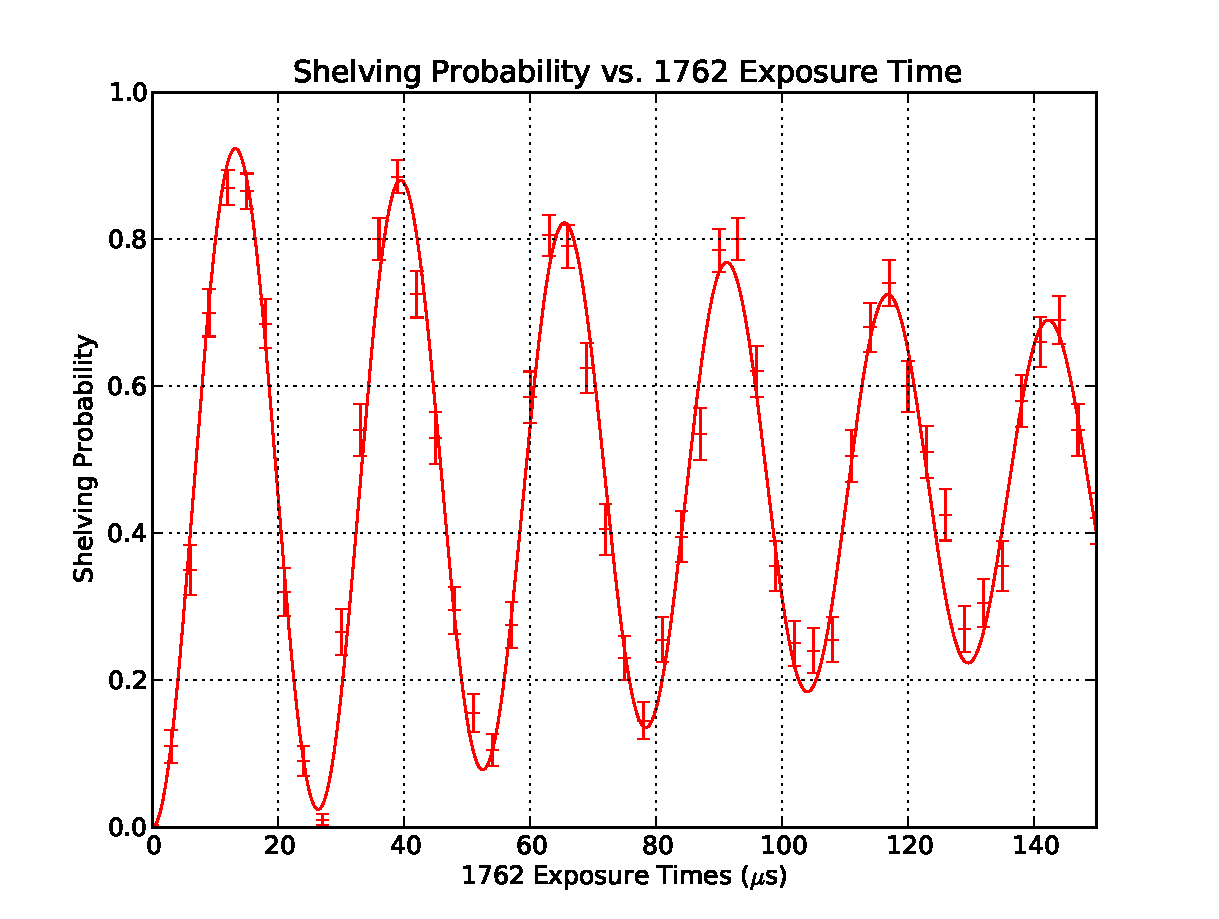
\includegraphics[width=0.7\textwidth]{HeatingRateT50000Orange}
	\caption[Rabi oscillations on the 1762~nm transition at different ion temperatures]{Rabi oscillations with different delays between the end of Doppler cooling and the beginning of 1762~nm laser exposure.  The contrast of the Rabi oscillations decays more quickly after a delay of 50~ms (bottom) than with no delay (top).}
	\label{fig:rabi-heating}
\end{figure}


\begin{figure}
	\centering
	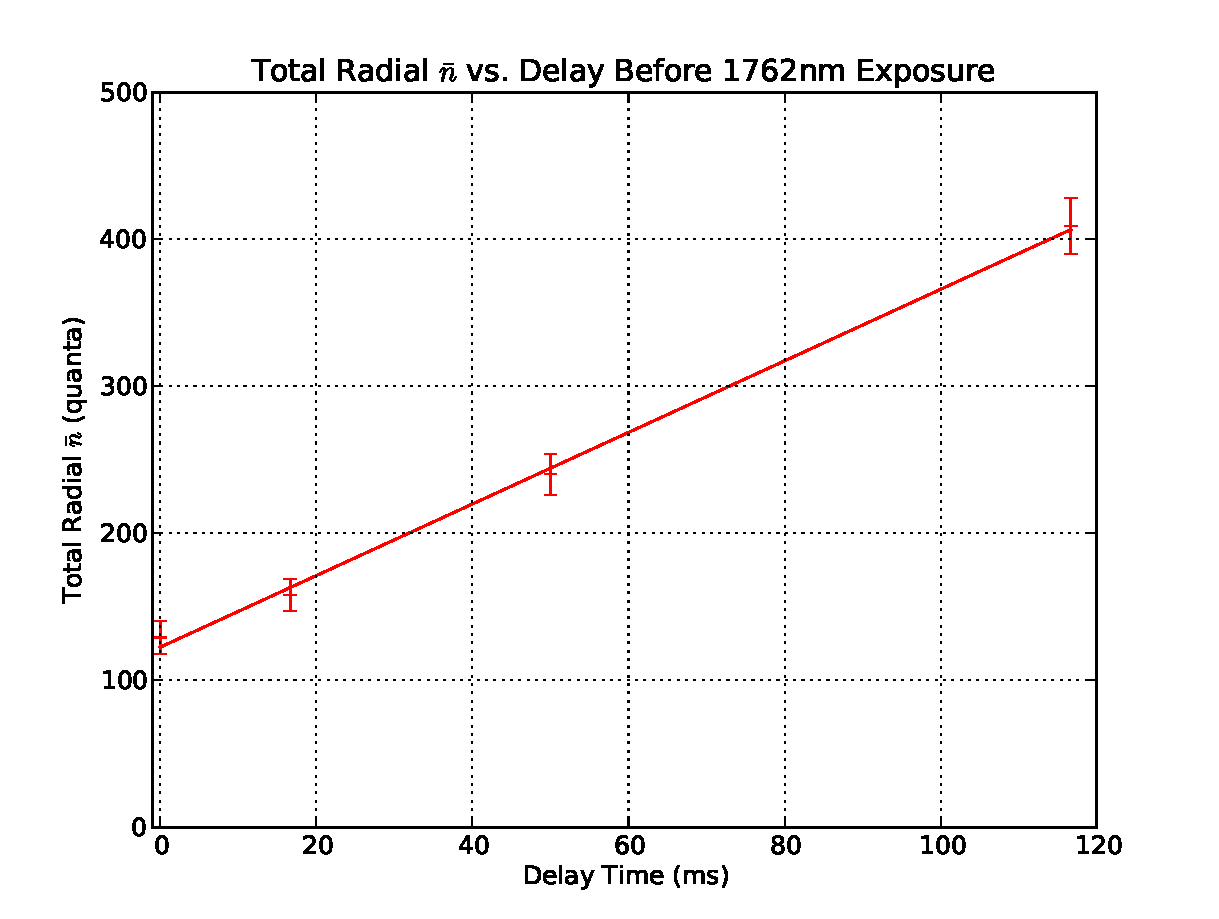
\includegraphics[width=0.8\textwidth]{HeatingRate}
	\caption[Heating rate of single barium ion without 1762~nm noise correction]{Heating rate of a single barium ion without correcting for 1762~nm frequency noise.  Total thermal radial mode average occupation number is plotted as a function of delay time during which the ion is not cooled.  A linear fit is shown with initial total radial average thermal occupation number of 122~quanta and a 2.43~quanta/ms heating rate.}
	\label{fig:heating-nonoise}
\end{figure}

Unfortunately, the initial temperature of the ion that we measured with this procedure was significantly hotter than expected.  Doppler cooling barium ions with 493~nm light should result in ion temperatures of $<$ 0.5~mK from Equation~\ref{eqn:doppler}. The measured initial temperature is approximately an order of magnitude higher at $\approx$ 60 quanta per radial mode of motion, which corresponds to $\approx$ 3.5~mK.  By carefully exploring the dependence of the decay of our Rabi oscillations with temperature we determined that our initial ion temperature is not actually this large.  Instead, there is an increased loss of contrast caused by frequency variations in our 1762~nm laser.

This laser is locked to a 500~kHz linewidth cavity by a locking circuit that stabilizes it to within a few percent of the cavity linewidth.  The small residual error still corresponds to a frequency modulation of the laser with a modulation depth of 10~kHz, but the timescale of the modulation is very slow compared to the duration of the pulses we apply to the ion.  The result is that every run of our Rabi flop experiment sees an approximately constant frequency drawn from this 10~kHz wide distribution of frequencies.  By sampling from this distribution in the fit function we can correct the measured Doppler temperature for this additional effect.  The shelving probability, $P_{\mathrm{shelved}}$, is then given by
\begin{eqnarray}
	P_\mathrm{shelved}(t) &=& \int_\omega \frac{1}{\sigma \sqrt{2 \pi}} e^{-\frac{(\omega - \mu)^2 }{2 \sigma^2}} \sum\limits_{n=0}^\infty \frac{1}{\bar{n} + 1} \left( \frac{\bar{n}}{\bar{n} + 1} \right)^2 \frac{s \Omega^2}{W^2} \sin^2 \left( W (1 - \eta^2 n) \frac{t}{2} \right) \\
	W(\omega)^2 &\equiv& \Omega^2 + (\omega - \omega_\mathrm{transition})^2
\end{eqnarray}
where $\sigma$ is the width of the residual frequency noise ($\approx$ 10~kHz), $\mu$ is the center frequency of this distribution which is approximately equal to $\omega_\mathrm{transition}$ which is the center of the 1762~nm transition, and $\Omega$ is the Rabi frequency ($\approx$ 50~kHz with our achievable laser power).  The resulting curve also exhibits a loss of contrast on the 100~$\mu$s time scale.

The fit parameters are the Rabi frequency $\Omega$, the optical pumping efficiency $s$, and the sum of the radial average thermal occupation numbers $\sum_i \bar{n}_i$.  In Figure~\ref{fig:heating} we have fit this new model to the same data and the heating rate of the radial modes is again approximately linear, with an initial temperature that is reasonable for a Doppler cooled barium ion.  The linear fit shown corresponds to an initial $\sum_i \bar{n}_i$ = 17~quanta, with a heating rate of 2.84~quanta/ms.  The corresponding minimum Doppler temperature is $\approx$ 1~mK, which agrees reasonably well with the theoretical minimum given the saturation of the 493~nm transition and the complicating effect of the 650~nm repump laser.  We will use these single ion measurements to evaluate our results with ion chains in the next section.  We expect that the heating rate per ion should be approximately constant.

\begin{figure}
	\centering
	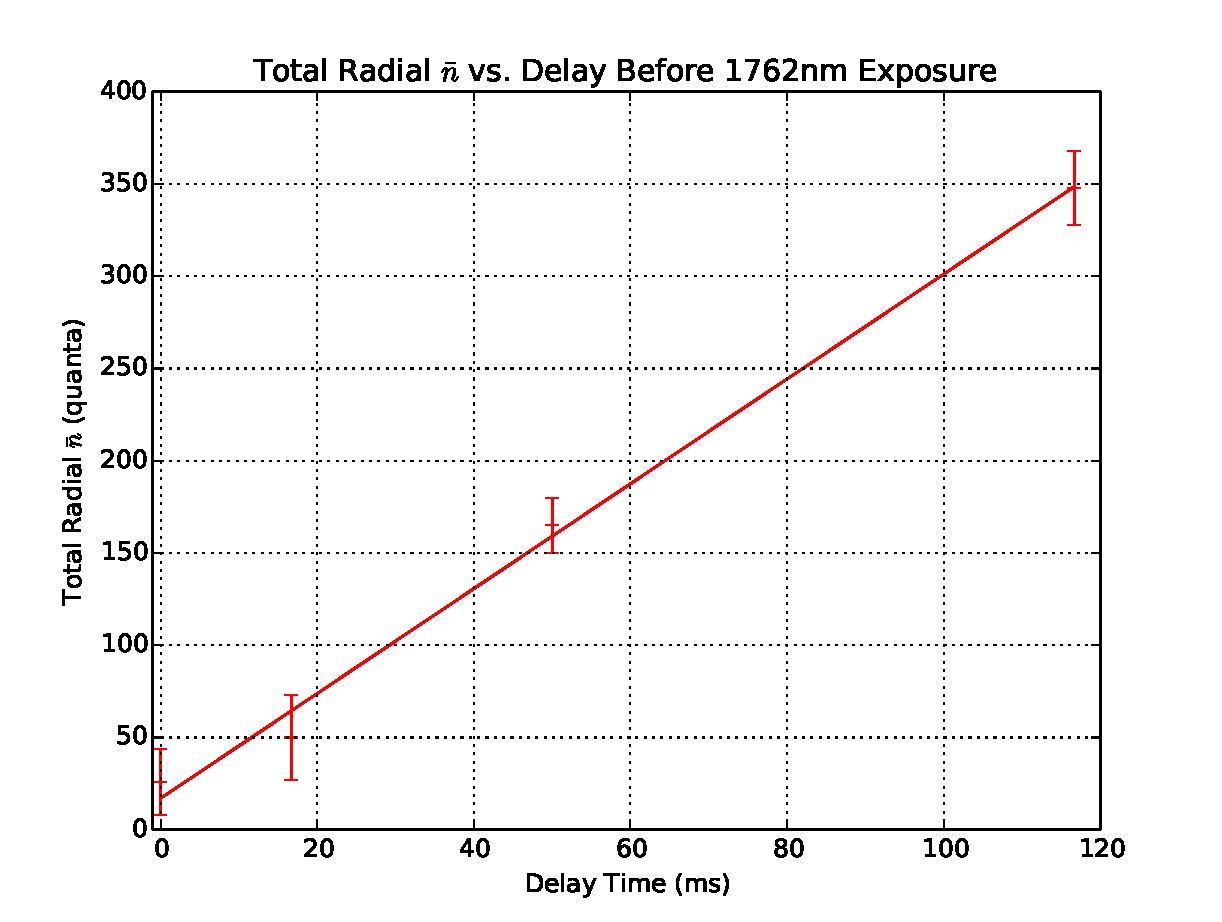
\includegraphics[width=0.8\textwidth]{HeatingRateNoise}
	\caption[Heating rate of single barium ion]{Heating rate of a single barium ion in a linear rf trap.  Measured radial motional average occupation numbers as a function of the period of time the ion was allowed to heat before the 1762~nm pulse began.  A linear fit is shown with initial radial average thermal occupation number of 17~quanta and a 2.84~quanta/ms heating rate.}
	\label{fig:heating}
\end{figure}

\section{Mixed Species Ion Chains}
\label{sec:mixed-modes}

In order to analyze the temperatures of mixed species chains, we first need to understand the normal mode structure of a chain of ions with different masses.  The normal modes for any given number of each species of ion and any ordering of those species can be calculated through classical mechanics techniques.  When the dynamics are much slower than the rf period, the Mathieu equation can be ignored and the trapping potential can be written as a simple harmonic oscillator.  The trapping potential is then
\begin{equation}
	V_\mathrm{trap} = \sum\limits_{i=1}^N \frac{1}{2} m_i \omega_x^2(m_i) x^2 + \frac{1}{2} m_i \omega_y^2(m_i) y^2 + \frac{1}{2} m_i \omega_z^2(m_i) z^2 \mathrm{,}
\end{equation}
where $N$ is the number of ions in the trap, $m_i$ is the mass of ion $i$, and $\omega_z$ is the axial confinement generated by the dc electrodes that is necessarily weaker than the radial secular frequencies $\omega_x$ and $\omega_y$.  The trap frequencies are a function of the ion mass as described in Equations~\ref{eqn:axialfreq} and \ref{eqn:radialfreq}.  The trap potential is modified by the Coulomb interaction between the ions
\begin{equation}
	V_\mathrm{coulomb} = \frac{1}{2} \sum\limits_{i = 1}^N \sum\limits_{j \ne i} \frac{1}{4 \pi \epsilon_0} \frac{q^2}{ \left| \vec{x}_i - \vec{x}_j \right| } \mathrm{,}
\end{equation}
where $q$ is the charge of an ion.

At the minimum of the potential, the linear terms are zero and the potential can be approximated by
\begin{eqnarray}
	V &=& \sum\limits_{i=1}^{3N} \sum\limits_{j=1}^{3N} V_{ij} x_i x_j \\
	\label{eqn:mixedtrap}
	V_{ij} &\equiv& \frac{1}{\sqrt{m_i m_j}} \frac{ \partial }{ \partial x_i } \frac{ \partial }{ \partial x_j } ( V_\mathrm{trap} + V_\mathrm{coulomb} ) 
\end{eqnarray}
where we have neglected a constant offset and allowed $i$ and $j$ to represent the $\hat{x}$, $\hat{y}$, or $\hat{z}$ direction of any one of the N ions.  Anharmonic terms can be taken into account by evaluating higher derivative tensors and using perturbation theory \cite{Home:11}.  The equations of motion for the harmonic terms are given by
\begin{equation}
	\ddot{x_i} + V_{ij} x_j = 0 \mathrm{.}
\end{equation}
There are 3N solutions which take the form of independent harmonic oscillators.  Each harmonic oscillator corresponds to motion along one of the eigenvectors of the matrix $V_{ij}$ with an angular frequency $\omega_\alpha$ equal to the square root of the corresponding eigenvalue.  We can write these solutions as
\begin{equation}
	\vec{x}_{\alpha}(t) = \hat{e}_{\alpha} \cos(\omega_\alpha t)
\end{equation}
for each normal mode $\alpha$, where $\hat{e}_\alpha$ is a unit length eigenvector of $V_{ij}$.  The analysis of sideband transitions still carries through with one small modification.  The separate motional state operators for each ion and each mode now carry the corresponding eigenvector component as a scalar multiplier that reduces the motion of each individual ion.  This effect can be accounted for by defining our Lamb-Dicke parameter for each mode $\alpha$ and ion $i$ to be $\eta_{\alpha, i} = \hat{e}_{\alpha}^i x_{\alpha, 0} k_x$, where $x_{\alpha, 0} = \sqrt{ \frac{\hbar}{2 m \omega_\alpha} }$.

We can scan the frequency of the 1762~nm laser over these radial modes following almost the same procedure used for a single barium ion.  One difference is that state detection must be done with our EMCCD camera instead of with the PMT.  The PMT has no spatial sensitivity and cannot distinguish which ions in the chain are bright.  Since we need to independently build statistics of each ion's state, we must be able to distinguish which ions are shelves in each experimental run.  I have developed software that integrates our experiment with the EMCCD camera and automatically performs this analysis.

An additional difference is that data must be collected when the ions are ordered in a particular configuration.  The normal mode structure changes depending on the ordering of the ion species and the numbers of each ion.  This structure must be constant in each experimental run.  In the future, this work can be done in microfabricated traps where dc control voltages can be used to separate, reorder, and merge ions.  At the moment, the ions are randomly reordered by shuttering the Doppler cooling lasers and allowing the ions to heat until the ion crystal melts.  When the ions recrystallize their order randomly changes.  This procedure must be repeated until the desired order is achieved at random.   It becomes more unlikely to reach the correct configuration as the number of possible configurations increases which is the current limiting factor in the number of ions we can use in these experiments.

We have performed initial characterizations of chains of two barium and two ytterbium ions.  This chain length is short enough that we can achieve the desired ion ordering easily enough to take reasonable amounts of data.  We are most interested in how effectively the ytterbium ions can be kept cooled by only Doppler cooling the barium ions.

\begin{figure}
	\centering
	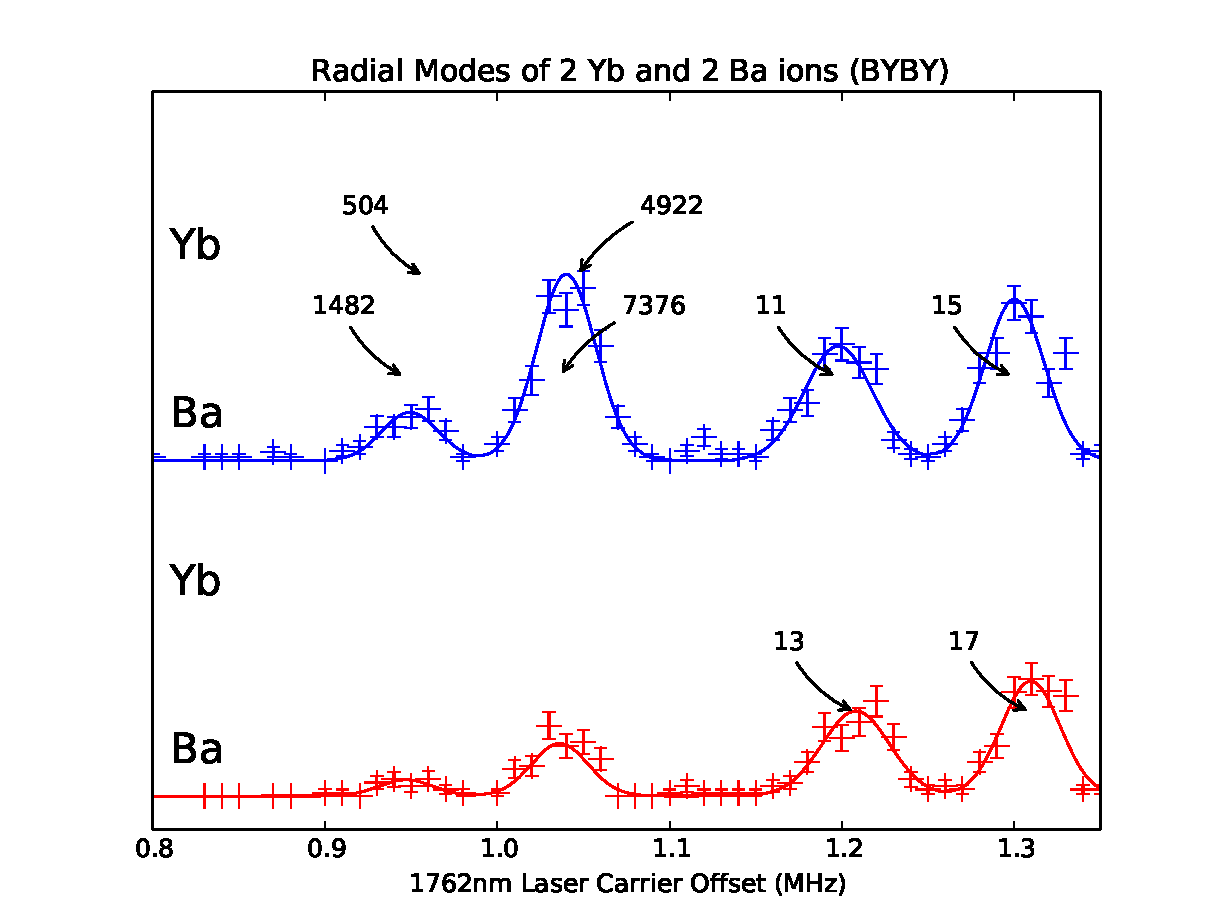
\includegraphics[width=0.7\textwidth]{RadialScanBYBY}
	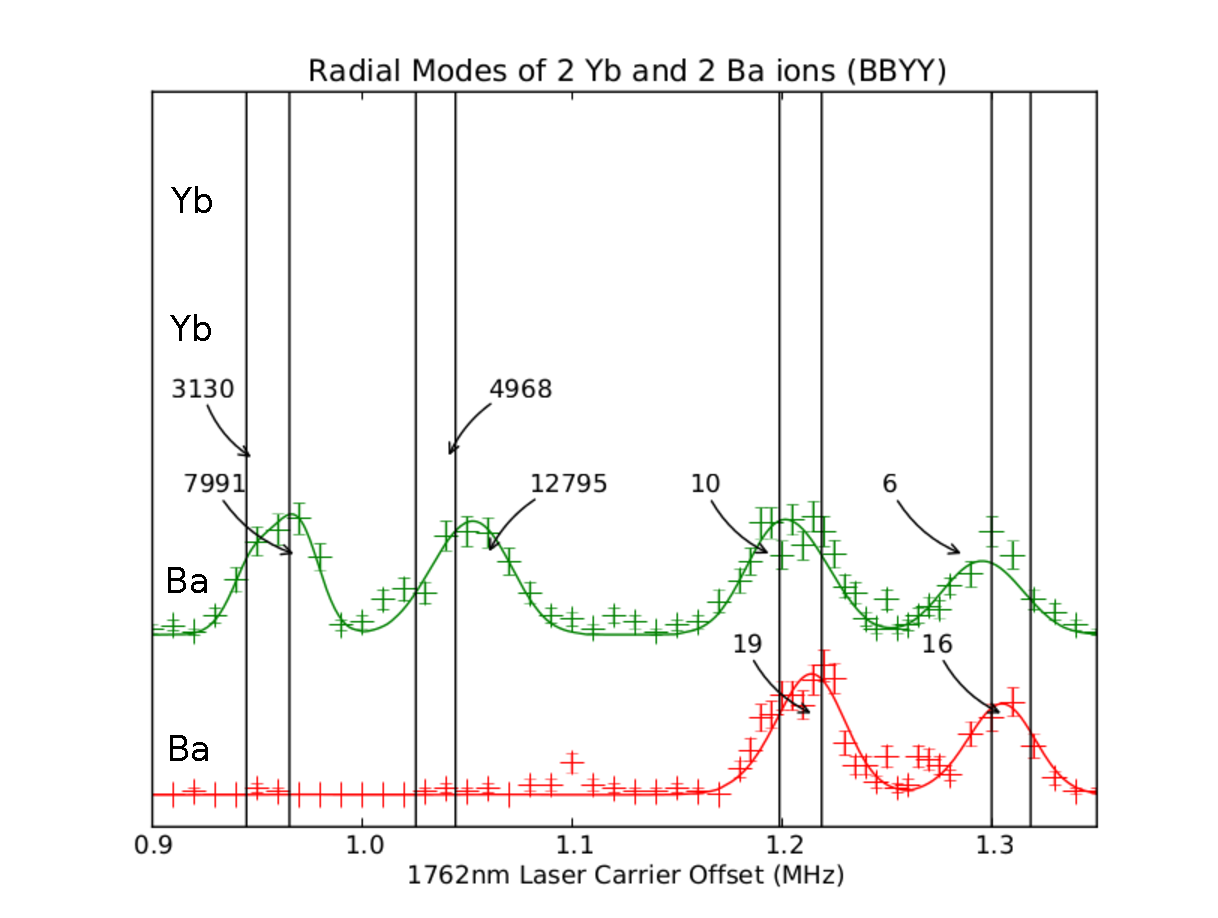
\includegraphics[width=0.7\textwidth]{RadialScanBBYY}
	\caption[Frequency scan over 1762~nm radial sidebands in a barium-ytterbium chain]{Frequency scan over the 1762~nm radial sidebands in a barium-ytterbium mixed species chain.  Predicted radial mode frequencies are shown by vertical lines while measured motional modes are labeled by arrows, along with their $\bar{n}$.  The vertical positions of the data curves show the locations of the barium ions in the chain with blank horizontal spaces representing the unaddressed ytterbium ions.  The top panel shows a Ba-Yb-Ba-Yb configuration and the bottom panel shows a Ba-Ba-Yb-Yb configuration.}
	\label{fig:radial-byby}
\end{figure}

After we have achieved the desired ion species configuration, we scan the frequency of the 1762~nm laser over the blue radial mode sidebands.  We limit the exposure time of the laser such that the shelving probability does not exceed 35\% allowing us to fit each peak to the weak excitation limit using Equation~\ref{eqn:shortpulses}.   In this limit, the shelving probability is given by
\begin{equation}
	P_\mathrm{shelve}(\omega) = \frac{1}{4} \eta_{\alpha, i}^2 \bar{n} \Omega_i^2 \frac{ \sin^2( (\omega - \omega_\alpha) t / 2) }{ (\omega - \omega_\alpha)^2 / 4 } \mathrm{,}
	\label{eqn:sidebands}
\end{equation}
where $\Omega_i$ is the Rabi frequency of the 1762~nm laser on ion $i$. In order to find $\Omega_i$ we also perform a Rabi experiment on the ion chain and determine the Rabi frequency for each ion by fitting to the resulting curve.  Again we have to deal with the frequency noise of the 1762~nm lock by allowing the 1762~nm frequency to vary over some range of frequencies.  Therefore, we actually fit the radial sideband curves to the integral of Equation~\ref{eqn:sidebands} over a Gaussian distribution of frequencies around a center frequency.  This frequency noise has the effect of broadening all of the radial modes and making it more difficult to fit the heights of modes close together in frequency.

The radial mode frequencies and eigenvectors are found from Equation~\ref{eqn:mixedtrap} following the numerical procedure described, but the measured radial mode frequencies display small, 10~kHz to 20~kHz, shifts from the theoretical frequencies.  We believe these shifts are due to small offsets in the error signal of the 1762~nm laser that occur when the laser is relocked.  The ZeroDer cavity that the laser is locked to also displays mechanical relaxation at a rate of 10~kHz/day, which explains some of the shifts because of the 10~hour experimental run time.  To accurately fit the peak heights we must also fit for the angular frequency of each mode, but the resulting frequencies are only shifted by 10~kHz to 20~kHz from the theoretical predictions.

First we will consider the case where the barium ions are maximally dispersed in the ion chain, i.e. the chain order is barium, ytterbium, barium, and ytterbium.  In top panel of Figure~\ref{fig:radial-byby}, a radial mode scan of this configuration is shown.  The two data curves are the probability of shelving the barium ion in that position as a function of the 1762~nm laser detuning.  The blank horizontal spaces correspond to the positions of ytterbium ions that are not addressed by any lasers.  The theoretically predicted radial modes given our independently measured trap secular frequencies are shown as black vertical lines.  The positions of the modes after the small frequency shifts are fit to them are indicated by the positions pointed to by the arrows, which label the fit $\bar{n}$ to each peak.  The four lowest frequency modes have large eigenvector motional components in ytterbium ions, but very small motional components for both barium ions.  It is clear from the labeled values of $\bar{n}$ that these modes are not being well cooled by the barium cooling lasers.  The mode frequencies, barium eigenvector components, and $\bar{n}$ for each mode in this configuration are given in Table~\ref{tab:byby}.  It is clear that there is a very large difference in the amount of motion that the last four modes have in barium ions than the first four.  We can also observe that having both eigenvector components be of the same magnitude does not decrease the number of quanta in the mode significantly, but even slightly increasing the maximum eigenvector component can have large effect.  Additionally, the participation of the barium ions in a given mode is increased when the base secular frequency for that direction is smaller.  

\begin{table}
\begin{tabularx}{1\textwidth}{ |>{\setlength\hsize{1\hsize}\centering}X|>{\setlength\hsize{1\hsize}\centering}X@{} >{\setlength\hsize{1\hsize}\centering}X|>{\setlength\hsize{1\hsize}\centering}X| }
	\multicolumn{4}{>{\centering\setlength\hsize{4\hsize} }X}{Ba, Yb, Ba, Yb Radial Mode Data} \tabularnewline
	Frequency (MHz) & 
	\multicolumn{2}{>{\centering\setlength\hsize{2\hsize} }X|}{ Barium Eigenvector Components } &
	$\bar{n}$ \tabularnewline
	\hline

	1.30 & 0.989 & 0.143 & 17 \tabularnewline
	1.29 & -0.144 & 0.989 & 15 \tabularnewline
	1.20 & 0.988 & 0.148 & 13 \tabularnewline
	1.19 & -0.150 & 0.987 & 11 \tabularnewline
	1.03 & 0.003 & 0.034 & 4913 \tabularnewline
	1.02 & 0.028 & 0.034 & 7427 \tabularnewline
	0.95 & 0.003 & 0.039 & 490 \tabularnewline
	0.94 & 0.033 & 0.041 & 1501 \tabularnewline
\end{tabularx}
\caption[Occupation number of modes in Ba-Yb-Ba-Yb chain]{Eigenvector components and occupation numbers for each mode in a chain of Ba-Yb-Ba-Yb ions.  The modes coupled strongly to ytterbium have much higher occupation numbers.}
\label{tab:byby}
\end{table}

When we move all of the barium ions to one side of the chain such that the order is barium, barium, ytterbium, ytterbium, we find the occupation numbers from Table~\ref{tab:bbyy}.  The temperature of the decoupled modes has increased substantially.  It is very clear from the eigenvector components of these modes and from Figure~\ref{fig:radial-byby} that the outermost barium ion is even more strongly decoupled.  It is fairly easy to conclude that for any reasonable chance of cooling all of these modes using barium ions, the barium ions will have to be interspersed along the length of the chain.  

\begin{table}
\begin{tabularx}{1\textwidth}{ |>{\setlength\hsize{1\hsize}\centering}X|>{\setlength\hsize{1\hsize}\centering}X@{} >{\setlength\hsize{1\hsize}\centering}X|>{\setlength\hsize{1\hsize}\centering}X| }
	\multicolumn{4}{>{\centering\setlength\hsize{4\hsize} }X}{Ba, Ba, Yb, Yb Radial Mode Data} \tabularnewline
	Frequency (MHz) & 
	\multicolumn{2}{>{\centering\setlength\hsize{2\hsize} }X|}{ Barium Eigenvector Components } &
	$\bar{n}$ \tabularnewline
	\hline

	1.31 & 0.866 & 0.500 & 16 \tabularnewline
	1.29 & -0.500 & 0.865 & 6 \tabularnewline
	1.20 & 0.865 & 0.501 & 19 \tabularnewline
	1.18 & -0.501 & 0.864 & 10  \tabularnewline
	1.03 & 0.002 & 0.022 & 12795 \tabularnewline
	1.01 & 0.002 & 0.029 & 4968 \tabularnewline
	0.95 & 0.002 & 0.026 & 7991 \tabularnewline
	0.93 & 0.002 & 0.035 & 3130 \tabularnewline
\end{tabularx}
\caption[Occupation number of modes in Ba-Ba-Yb-Yb chain]{Eigenvector components and occupation numbers for each mode in a chain of Ba-Ba-Yb-Yb ions.  The modes coupled strongly to ytterbium have much higher occupation numbers.}
\label{tab:bbyy}
\end{table}

In order to gain a simplified understanding of what this data tells us about the temperature of ions in mixed species ion chains, we have compared the $\bar{n}$ for each radial mode that is not cooled well by barium to its eigenvector components for barium ions.  The correlation between these variable seems to be strongest when we compare $\bar{n}$ to the maximum eigenvector component, $\max_{i,\mathrm{barium}} \left| \hat{e}_\alpha^i \right|$.  Plotting these variables against each other shows a strong correlation, with reasonable thermal occupation numbers only being reached when the eigenvector component is $\approx$ 0.04.

\begin{figure}
	\centering
	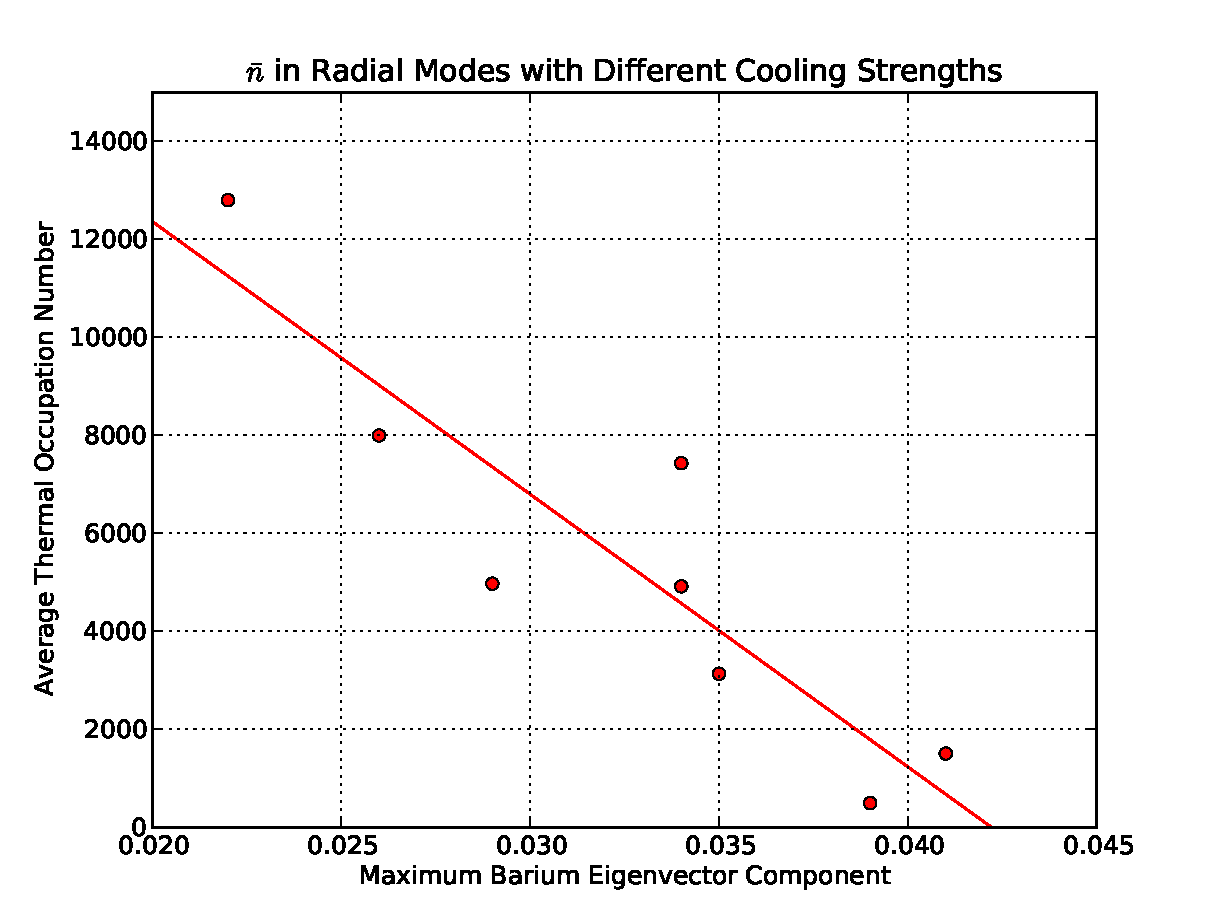
\includegraphics[width=0.8\textwidth]{RadialNBarEigenvectors}
	\caption[Radial mode occupation numbers for different barium ion motional couplings]{Radial $\bar{n}$ as a function of the maximum eigenvector component of the mode with a cooled barium.  The linear trend is given as a guide to the eye.}
	\label{radial-nbars}
\end{figure}

Obviously cooling ytterbium ions using only barium cooling lasers is not going to be as efficient as we would hope.  It seems that that our Doppler cooling is near optimal for barium ions, so it is unlikely that Doppler cooling alone will be able to perform any better than this.  There are still a few options for making progress however.  For the weaker of the two trap axes, we can see that the ytterbium modes are reasonably cold for chain configurations that are well mixed.  Only a few modes of the trap will need to be kept cold to perform entangling gates in ytterbium, and its possible the trap strengths and ion configuration can be arranged to make this possible.  Doing so will likely require the barium to be well distributed throughout the chain.

Investigating these problems for increasing numbers of ions should prove very interesting.  If the trends established above continue to hold it may still be possible to keep a few modes cold enough to be in the Lamb-Dicke regime and perform entangling operations in ytterbium.  Working with more ions will most likely involve moving this experiment to a surface electrode trap where the ordering of the ions can be easily controlled.  Scaling this experiment further in its current trap would be very difficult.

\section{Ion Species Reordering}
\label{sec:reordering}

Working with mixed ion species chains gives an experimenter the ability to determine when chains reorder.  Obviously when working with only a single ion species, the ions are indistinguishable and it is impossible to tell whether its order is the same as previously at any point in time.  We hypothesized that the reordering of ions would happen at a relatively constant temperature and therefore could provide a simple temperature or heating rate measurement.  To investigate this hypothesis we performed simulations of the motion of mixed ion species chains.

Heating in ion chains is difficult to simulate well because it often depends on random electric field noise which is difficult to integrate numerically.  Instead of simulating the heating process, the ions are initialized at the beginning of the simulation to a given temperature.  Depending on this initial temperature, we track the probability for them to reorder before they are cooled to somewhere near their ground state.  The initial temperature is modeled by initializing the ions velocity to the corresponding energy with a random direction.  The ions motion is then modeled subject to the differential equation
\begin{equation}
	m_i \ddot{\vec{x}}_i = \vec{F}_\mathrm{trap}(m_i) + \hbar \vec{k} \frac{\Gamma}{2} \frac{s}{1 + s + 4 \left( \frac{\delta + \vec{k} \cdot \dot{\vec{x}}}{\Gamma} \right)^2}	+ \sum\limits_{j \ne i} \frac{1}{4 \pi \epsilon_0} \frac{e^2}{ \left| \vec{x}_i - \vec{x}_j \right| ^3 } \left( \vec{x}_i - \vec{x}_j \right) \mathrm{,}
\end{equation}
where $\vec{x}_i$ is the position of the ion that began in position $i$, $\vec{F}_\mathrm{trap}$ is the harmonic trapping force that confine the ions, and $s$, $\Gamma$, $\delta$, and $\vec{k}$ are the saturation parameter, natural linewidth, detuning, and wavevector of the main Doppler cooling laser.  This differential equation is numerically integrated using the Boost odeint library\footnote{\url{http://www.boost.org/doc/libs/1_57_0/libs/numeric/odeint/doc/html/index.html}}.  Once the ions reach a sufficiently low energy, it is determined whether the ion species have reordered in a way that is experimentally detectable.  Figure~\ref{fig:reorderingpos} shows a sampling of the axial positions of a chain of ions from a single run of the simulation where the ions reorder.  Repeating this process several thousand times for several initial temperatures shows us that the probability to reorder changes relatively sharply with temperature.  Using a single quad-core desktop the runtime for performing 10,000 iterations of this procedure is almost a day because of the difficulty of integrating singular potentials and the long integration times used.

\begin{figure}
	\centering
	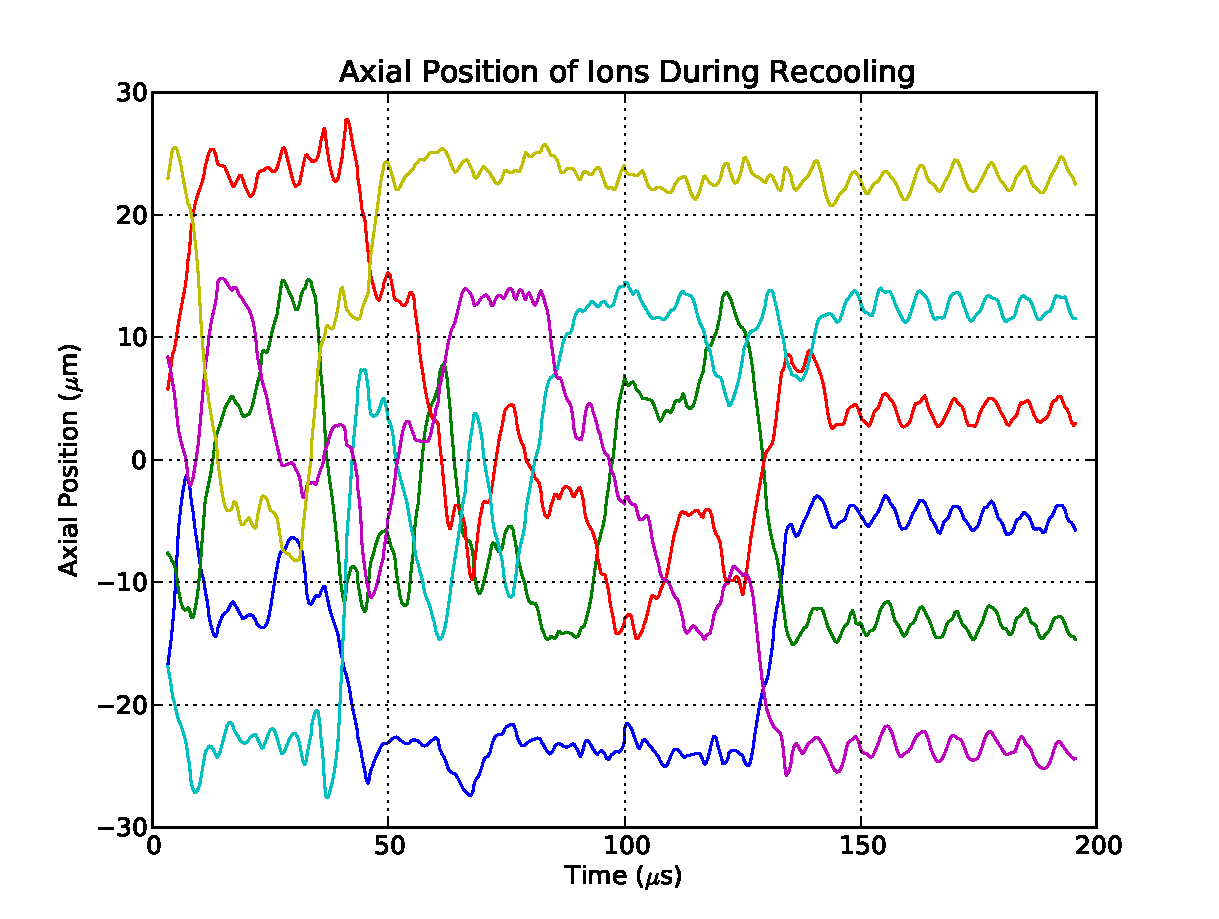
\includegraphics[width=0.8\textwidth]{ReorderingPositions}
	\caption[Simulated axial positions during Doppler recooling]{Simulated axial positions of trapped ions as function of time.  The ions are initialized with a large randomly directed velocity and are cooled by simulated Doppler cooling.  The numerical integration is performed by the odeint library.}
	\label{fig:reorderingpos}
\end{figure}

\begin{figure}
	\centering
	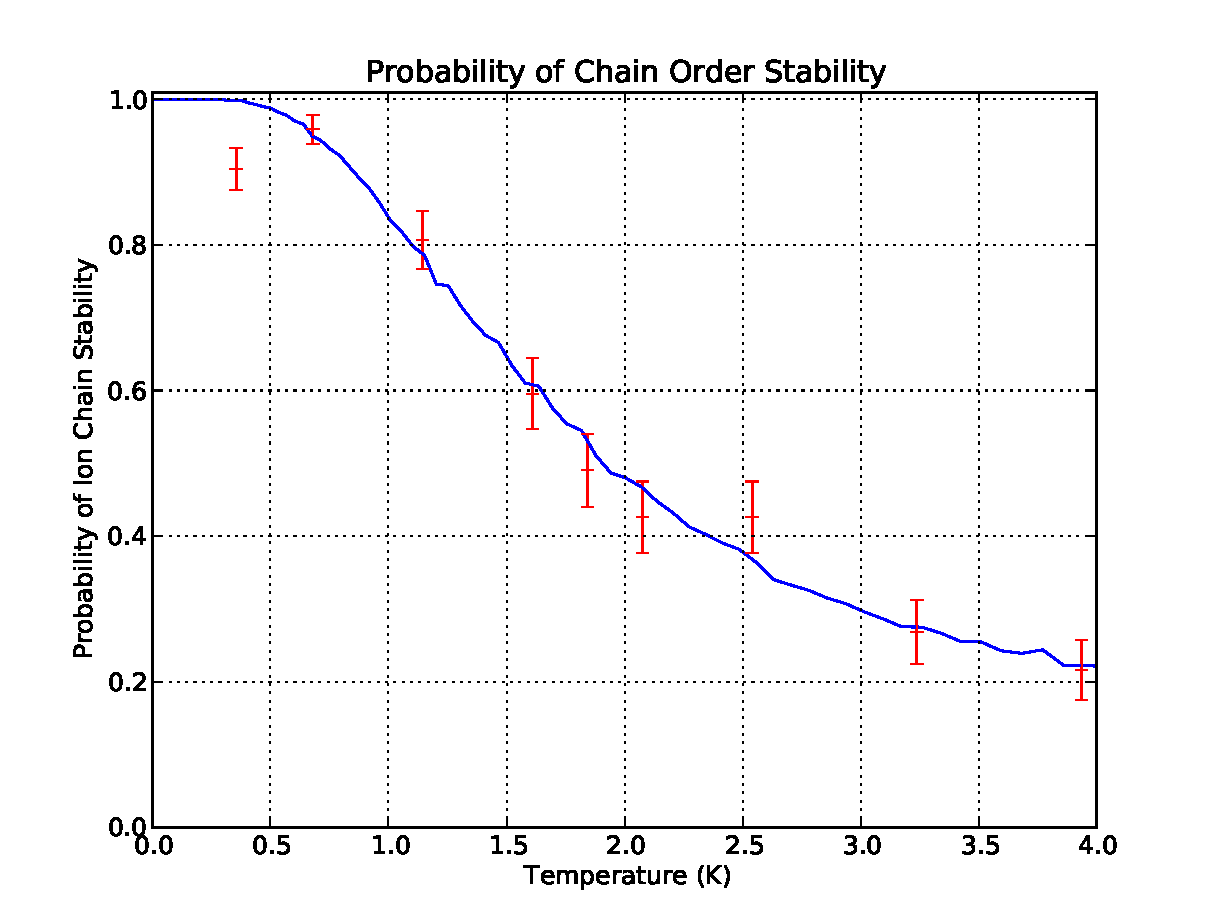
\includegraphics[width=0.7\textwidth]{Reordering81}
	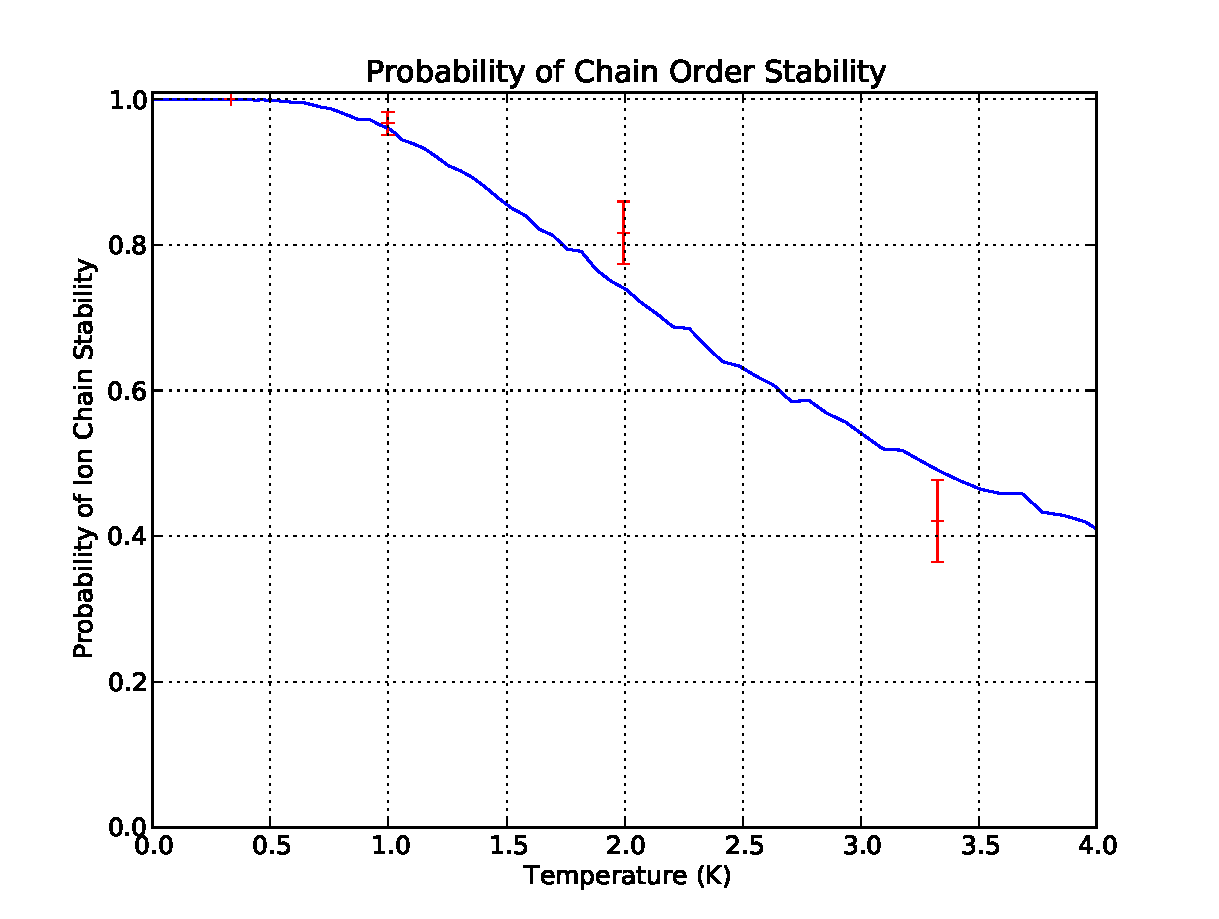
\includegraphics[width=0.7\textwidth]{Reordering61}
	\caption[Reordering probability of ion chains at different temperatures]{Reordering probability as a function of temperature.  The simulation results are shown in blue, while the red data points are taken at different uncooled times and then fit to temperatures using a linear heating rate.  For seven barium and one ytterbium ion (top) the initial temperature is 0.215~degrees Kelvin and the heating rate is 0.465~K/s.  For five barium and one ytterbium (bottom) the initial temperature is 0~K and the heating rate is 0.665~K/s.}
	\label{fig:reordering81}
\end{figure}

Experimentally, ion species reordering probabilities are very easy to measure.  Once again heating can be induced by allowing the ion to spend several hundred milliseconds to several seconds uncooled in the trap.  Using our EMCCD camera we image the ions before and after a given period of uncooled time.  The reordering probability is then extracted from a series of many such experiments.  In order to fit the collected data to the theoretical curve generated by the molecular dynamics simulation, we need to fit the initial temperature and heating rate of the ion chain.  

In Figure~\ref{fig:reordering81}, the resulting curves for an ion chain of 7 barium and one ytterbium ion are shown.  The fit indicates an initial temperature of 0.215~degrees Kelvin and a heating rate of 0.465~K/s.  For five barium ions and one ytterbium ion the initial temperature is 0~K and the heating rate is 0.665~K/s.  Obviously, this initial temperature is not physically realistic and is probably caused by the small amount of data taken using the smaller chain.  More data would have had to be taken to fit a reasonable initial temperature because its effect on the fit is relatively small.  The heating rate measurement should be reliable because it has a strong effect on the generated points.  A heating rate of 0.465~K/s corresponds to 8.07~quanta/ms for 1.2~MHz phonons.  This rate is 2.8 times larger than the radial mode heating rate of 2.84~quanta/ms for a single barium ion measured using Rabi flop decay, but it also includes the motional energy in the axial motional modes.  We have not directly measured the heating rate of these modes, but this total heating result seems reasonable because their heating rate is expected to be larger because of their lower frequency.

The advantage of this technique is that a single, fast measurement can quickly characterize the heating rate of the trap.  With the methods described earlier in this chapter several dozen data points each comprised of several hundred experimental runs must be performed to fit a function and determine the ions' temperature or heating rate.  Also, the configuration of the ion species must be controlled in order to analyze the same motional mode structure.  With the present method, collecting one or two data points near the maximum slope of the reordering probability can generate a quick measurement of the same quantity and, obviously, no effort to control the species configuration is necessary.  The reordering measurement also does not require any narrow transitions to be used, allowing traps to be quickly be characterized even before these additional lasers are aligned to them.

\begin{figure}
	\centering
	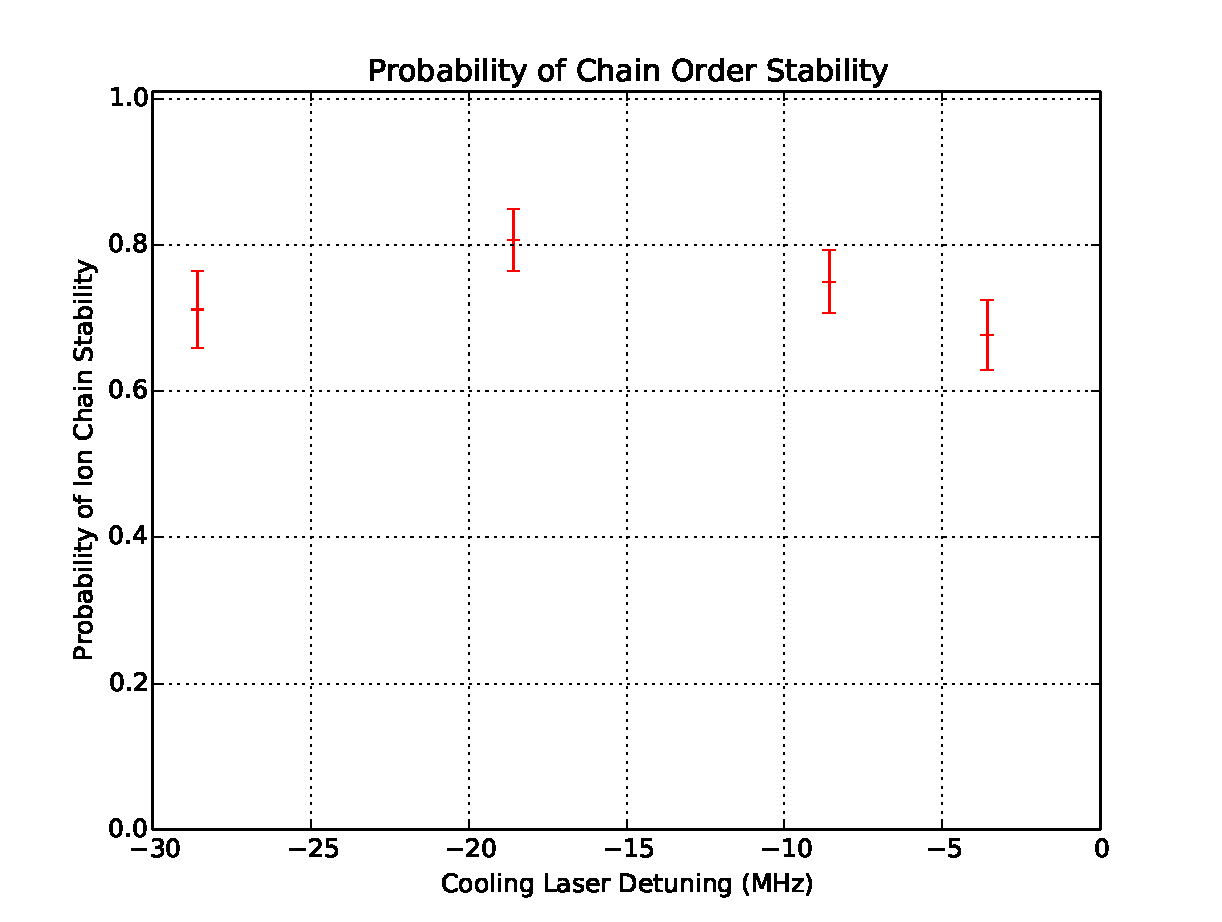
\includegraphics[width=0.8\textwidth]{ReorderingFreq}
	\caption[Reordering probability at different cooling laser detunings]{Reordering probability of a linear chain at different Doppler cooling laser frequencies.  The ions are allowed to heat for 2~seconds before the reordering is detected so that the rate of change of the reordering probability as a function of temperature is maximized. Lower probability of chain stability indicates lower cooling efficiency.  Although the variations are small, the results could be made statistically significant by taking more data.}
	\label{fig:reordering-freq}
\end{figure}

Since these measurements are so quick to carry out, it is also convenient to look at how our minimum temperature varies with our 493~nm laser frequency using this technique.  Figure~\ref{fig:reordering-freq} plots the reordering probability as a function of the detuning of this main barium cooling laser with the uncooled time in the experiment set to the maximal reordering slope.  Collecting data using this method took only a few minutes as compared to an hour or more to measure several curves with the other methods described.  For this reason, reordering measurements also serve as a good, fast indicator of cooling efficacy.  Although we saw earlier that this technique is not always a good measurement of initial temperature, when sitting on this maximal slope we can definitely see the effects of the Doppler cooling parameters.

In this chapter we have characterized the temperature and heating rate of barium and ytterbium ions in our trap in many different ways.  The benefit we were hoping to achieve in designing this system was the ability to continuously cool barium ions while performing quantum operations with ytterbium ions.  It certainly looks like that task is not going to be as easy as we had hoped.  In Chapter~\ref{sec:qcomp}, we found that we needed to be operating in the Lamb-Dicke regime where $\eta^2 \bar{n} \ll 1$ in order for M\o{}lmer-S\o{}rensen entangling operations to have high fidelity.  At the current average thermal occupation number of some of the modes and the expected $\eta$ for our laser we can expect $\eta^2 \bar{n} \approx 1$.  We are hopeful that by manipulating additional trap parameters in surface traps and using additional barium ions we can lower these temperatures, but if necessary we can also perform these entangling gates using the better coupled axial modes.  There are still many different possible degrees of freedom to explore in this new system.


\chapter{Quantum Operations}
\renewcommand{\curdir}{raman}
\label{sec:raman}

\graphicspath{ {\curdir/Graphics/}  }

As we make progress towards effectively cooling these ion chains we want to begin exploring how quantum operations can be engineered in them.  We have begun performing single qubit quantum gates with barium ions in our system, and are preparing the necessary infrastructure to being characterizing entangling gates.  Currently, our single qubit gates are driven with resonant rf fields, but we are developing a Raman laser system to perform these gates that will have single qubit addressability and large enough Lamb-Dicke parameter to also perform two qubit entangling gates.  We will begin by characterizing these gates in barium ions in our mixed species chains, but eventually transition to the architecture described previously.

\section{Zeeman Transitions}
\label{sec:zeeman}

The Zeeman qubit I have described in barium, as well as the hyperfine qubit in ytterbium, can be coherently controlled by applying rf or microwave magnetic fields to the ions.  In our group we have some traps that have been designed to accommodate applying large amplitude oscillating magnetic fields to ions by placing copper transmission lines along paths inside of the vacuum chamber near the ion.  Our current quantum information vacuum chambers were not designed to incorporate this feature, and for the moment we are applying the fields from the outside.

We have demonstrated our ability to find and drive Zeeman transitions in single barium ions using an external field coil driven by a Stanford SRS-345 frequency source.  The field coil is composed of approximately 20 turns of copper wire and is located on our imaging viewport approximately 1~cm from the ion.  The rf can be crudely coupled onto this coil by making a resonant circuit by adding capacitance to cancel the inductance of the coil near the Zeeman transition frequency.

The experimental procedure to observe these transitions again begins by switching the cooling lasers to perform optical pumping and pumping the ion into the $m_J = -\frac{1}{2}$ level of the ground state. The cooling lasers are then shuttered and we attempt to drive a Zeeman transition by applying resonant rf at our Zeeman transition frequency $\omega$ = $2 \pi \times$ 14.610~MHz to the field coil.  After this attempt, we apply a $\pi$-pulse of 1762~nm light to drive the $m_J = -\frac{1}{2}$ level to the $m_J = -\frac{1}{2}$ level of the 5D$_{5/2}$ shelved state with a probability of approximately 90\%.  Finally, we reactivate the cooling lasers and the ion fluoresces if it has not been successfully shelved.

For our initial characterization of this process, we have only been able to apply relatively small magnetic field amplitudes to the ion.  Figure~\ref{fig:zeeman-rabi} shows the shelving probability as a function of the exposure time of our rf source.  The beginning of a Rabi oscillation is clear, but then the frequency and amplitude of the transition begin to change.  These changes are due to the changing magnetic field in the trap because of the changing ac wall phase.  All of our magnetically sensitive experiments are triggered to begin on a maximum of the ac wall voltage, but since this experiment lasts for several milliseconds we begin to see the magnetic field shift.  Without magnetic shielding it is almost impossible to avoid having a large changing magnetic field caused by the current draw of all of the lab electronics.

\begin{figure}
	\centering
	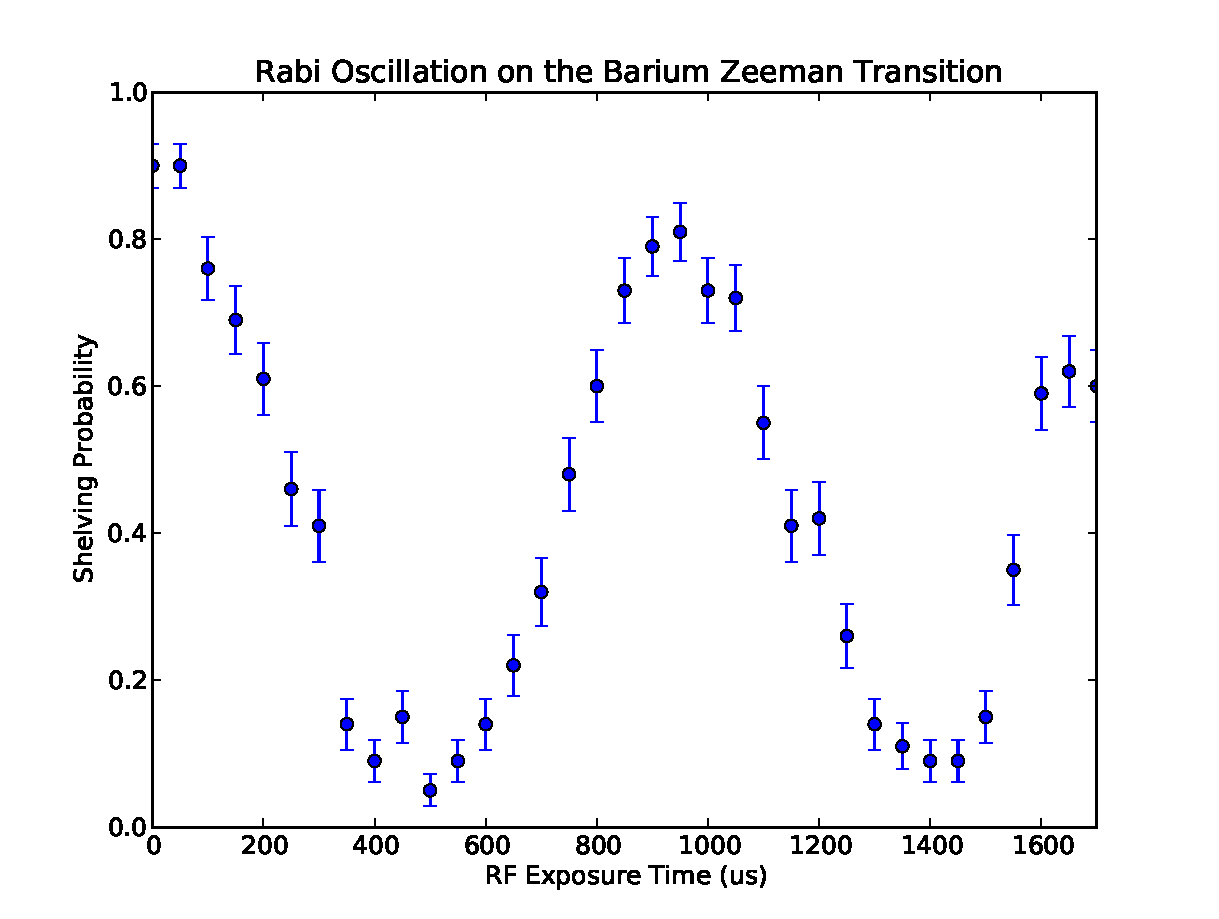
\includegraphics[width=0.8\textwidth]{ZeemanRabi}
	\caption[Rabi oscillations between Zeeman levels of the ground state of \ba]{Rabi oscillations between the \ba ground state Zeeman levels.  The probability of driving a 1762~nm transition from the Zeeman level the ion was initialized to is shown as a function of exposure time of rf current resonant with the Zeeman energy splitting.  The complicated behavior is caused by magnetic field shifts from the ac wall current.}
	\label{fig:zeeman-rabi}
\end{figure}

The fidelity of this qubit operation is currently low in our setup, but it demonstrates that we have the infrastructure to support these kinds of operations.  In other traps, my group has shown Rabi oscillations between these levels with 600~ns $\pi$-pulses and fidelities greater than 99\%. The fidelity in our setup could be quickly improved by using amplifiers and resonators to apply a stronger magnetic field to the ion.  Increasing our magnetic field would decrease the gate operation time and significantly reduce the size of the magnetic field drift.  Our maximum shelving probability could also be significantly improved by carefully improving our optical pumping efficiency and the 1762~nm $\pi$-pulse fidelity.  In actual quantum information processing, we plan to drive our single qubit gates using optical Raman transitions and therefore it is not necessary to optimize the fidelity of these rf-driven gates.  

\section{Raman Transitions}
\label{sec:raman-trans}

The difficulty with performing qubit rotations using resonant rf or microwaves is that the energy separation between ideal qubit levels can often be very small.  Therefore, near resonant radiation will have a long wavelength and be difficult to address onto single ions.  For example, the hyperfine qubit in $^{171}$Yb$^+$ has $\omega =$ 12.643~GHz, which corresponds to a wavelength of approximately 2.5~cm.  Typical ion separations in a single trapping region are 5~um to 10~um.  For performing quantum algorithms where we need to perform different rotations on adjacent qubits, we will need to use different techniques.  

It is possible to generate spatially varying microwave field intensities on the micron level using several electrodes on a surface trap geometry which enables single qubit addressing \cite{Warring:13}.  The energy difference of the qubit levels can also be varied by applying large magnetic field gradients to ion chains which enables frequency addressing single qubits \cite{Wang:09}.  Both of these techniques involve adding control electrodes to surface traps, but can achieve reasonably low crosstalk of a few percent or less.

We are planning to instead use optical Raman transitions to implement single- and multi-qubit gates.  Using optical Raman transitions is advantageous because the lasers driving them can easily be focused onto individual ions, and the photons absorbed and emitted carry enough momentum to usefully couple to the motion of the ions.  The interaction between optical fields and the motional modes of the trap is still characterized by the Lamb-Dicke parameter $\eta$ = $k_\mathrm{photon} x_\mathrm{ion}$.  We are planning to use a 532~nm laser to drive these transitions on our $\approx$ 1.2~MHz radial motional modes, which results in $\eta \approx$ 0.05.

\begin{figure}
	\centering
	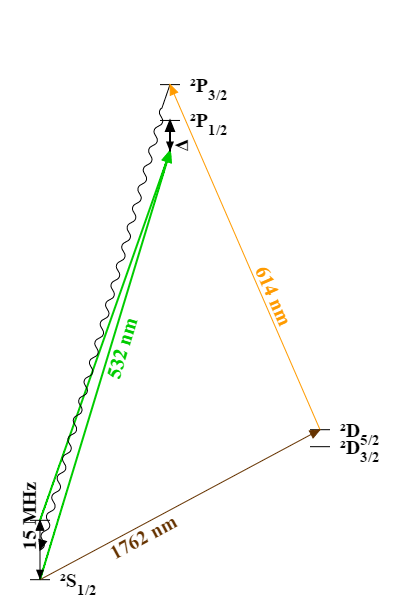
\includegraphics[width=0.5\textwidth]{ba-qcomp-lasers}
	\caption[Energy level diagram of Ba$^+$ quantum computation lasers]{Energy level diagram of Ba$^+$ including ground state Zeeman levels (not to scale) and relevant lasers.  Raman transitions can be driven using two 532~nm beams with a relative detuning equal to the Zeeman energy spacing.  Readout will still be performed using the 1762~nm laser.}
	\label{fig:ba-qcomp}
\end{figure}

For a pair of monochromatic light fields the Rabi frequency for Raman transitions can be written as 
\begin{equation}
	\Omega = \frac{ \left| \vec{\mu}_1 \cdot \vec{E}_1 \right| \left| \vec{\mu}_2 \cdot \vec{E}_2 \right| }{ \hbar^2 \Delta } \mathrm{,}
\end{equation}
where $\vec{\mu}_i$ are the electric dipole moment coupling the two Zeeman qubit levels to an intermediate level in the 6P$_{1/2}$ or 6P$_{3/2}$ state, $\vec{E}_i$ are the electric field magnitude and polarization for the two beams, and $\Delta$ is the detuning of each beam from the excited state.  Our detunings $\Delta$ are $2 \pi \times$ 44.5~THz from the 6P$_{1/2}$ state and $2 \pi \times$ 95.4~THz from the 6P$_{3/2}$ state.  However, our 532~nm source is not monochromatic, since the light is provided by a mode-locked laser.

The electric field from a mode-locked laser can be described by
\begin{equation}
	\vec{E}(t) = \vec{E}_0 \sum\limits_{n=0}^\infty f( t - n T ) \cos( \omega t + k_x x )
\end{equation}
where $\vec{E}_0$ is the electric field magnitude and polarization, $\omega$ is the center frequency of the laser, the function $f$ describes the pulse shape of the laser, and $T$ is the time period between pulses.  In an optimal mode-locked laser, $f(t) \propto \sech( \pi t / \tau )$, where $\tau$ is the time duration of the pulses.  Taking the Fourier transform of this field we can find that it has many sharp spectral components separated by the repetition rate of the laser, $\omega_R = 2 \pi / T$, in a $2 \pi / \tau$ bandwidth around $\omega$.  These ``comb teeth'' can be used to drive narrow atomic transitions \cite{Hayes:10}.  The frequency width of these teeth, $\omega_R / N$, is controlled by the number of pulses, $N$, applied to the ion.

\begin{figure}
	\centering
	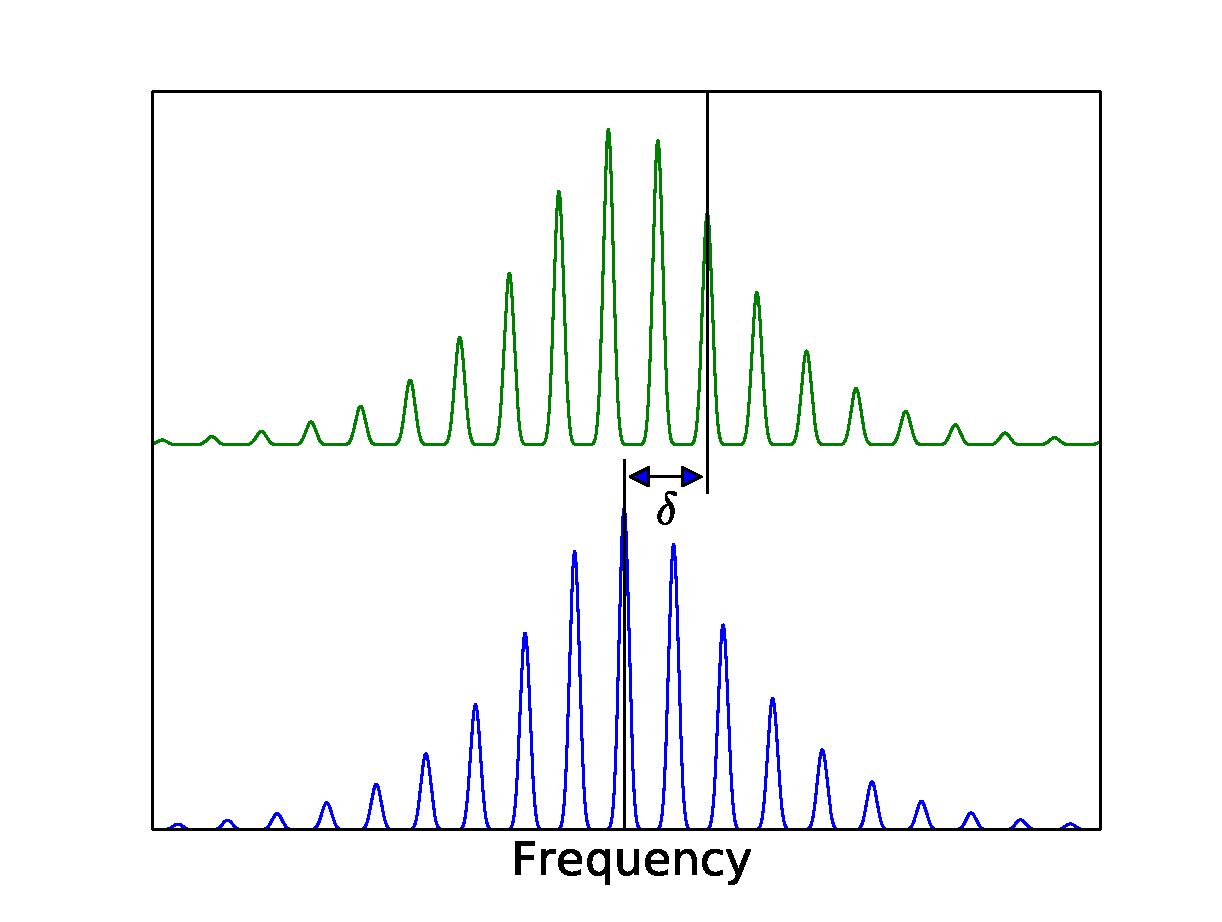
\includegraphics[width=0.7\textwidth]{ModelockedSpectrum}
	\caption[Frequency spectrum of a series of pulses from a modelocked laser]{Frequency spectrum of a series of pulses from a modelocked 532~nm laser.  The comb teeth are spaced by the repetition rate of the laser, and can be made more narrow by applying more sequential pulses to the ion.  The two pulse trains are detuned from one another by an AOM, and Raman transitions can be driven for any frequency $\delta$ equal to a multiple of the repetition rate plus or minus the AOM frequency.}
	\label{fig:modelocked}
\end{figure}

We will be using these comb teeth to drive Raman transitions between our qubit levels.  Therefore we require that the bandwidth of the laser is significantly larger than our qubit energy spacing such that many of the comb teeth can contribute to driving the transition.  By independently frequency shifting two beams from the laser by $\delta$, we will tune their frequency difference such that $\omega_\mathrm{qubit} = m \omega_R + \delta$ for some integer $m$. The resulting Raman transition will have a coupling strength given by
\begin{eqnarray}
	\Omega &=& \sum_n \frac{ \mu^2 E_n E_{n-m} }{ \hbar^2 \Delta } \\ 
	&\approx& \frac{\omega_R \tau}{2\pi} \frac{\mu^2 E_0 ^2}{\hbar^2 \Delta}
	\label{eqn:ramanapprox}
\end{eqnarray}
where $E_n$ is the electric field magnitude of comb tooth n and can be found from f.  The approximation is valid when $\omega_\mathrm{qubit} \tau \ll 1$ such that most of the comb teeth have a corresponding comb tooth at the correct detuning.  By simultaneously driving two Raman transitions with detunings of $\omega_\mathrm{qubit} \pm \delta$ on two ions, with $\delta \approx \omega_x$, we can use this laser to generate entanglement between ions using the M{\o}lmer-S{\o}rensen gate.  For our 532~nm light driving Raman transitions in barium, we must consider coupling through both the 6P$_{3/2}$ and the 6P$_{1/2}$ state.  We estimate that given our current laser power and focusing constraints, we can expect to drive carrier Raman transitions at a rate of $\Omega \approx$ 50~kHz.  The M{\o}lmer-S{\o}rensen coherent two qubit operation can be driven at a rate of $2 \eta \Omega \approx$ 5~kHz.

We will be using a mode-locked diode-pumped ND:YVO$_4$ laser to provide the optical beams.  This laser was originally a multimode CW pump laser for a Ti:Sapphire mode-locked laser, but it has been modified to support mode-locked operation itself.  Mode-locked operation is favored by a semiconductor saturable absorber end mirror that has been added to the laser cavity.  In addition, the cavity had been modified to produce the necessary tight focus on the saturable absorber \cite{Schlatter:04, Sun:10}.  The laser produces 2~W of optical power at 1064~nm that we frequency double using a LBO crystal in a single pass configuration to 500~mW of 532~nm light.  The output pulses were measured using an autocorrelator to have 17~ps duration and our repetition rate is approximately 150~MHz.

In order to drive Raman transitions using this system we need to split the pulse train into two beams and frequency detune these beams from each other (see Figure~\ref{fig:modelocked}).  We have accomplished this using two AOMs.  A base 220~MHz signal is generated by an HP-8640B signal generator and then split into two paths by a rf power splitter.  One path continues directly to a high speed rf switch, while the other is mixed with a computer controlled Stanford Research Systems DS345 20~MHz signal generator, resulting in signals at 200~MHz and 240~MHz, and then sent to a different switch.  Both paths are then amplified to approximately 1~W and sent to separate 200~MHz AOMs.  The bandwidth of the amplifier and the AOM severely attenuates the 240~MHz signal from the mixer leaving the two AOMs to be driven by 200~MHz and 220~MHz signals, respectively.  The common mode 220~MHz signal has no effect on Raman transitions and so the stability only depends on the DS345 signal and there is no need to phase lock two rf sources together.  This optical setup is operational with both beams controlled by the AOMs and focused into the trap.  The path length difference between the two beams is set by a linear delay stage and has been measured to approximately overlap the pulses in from the two paths.  Since we know the energy separation of the Zeeman levels because we have directly driven the the transition between them, there are no remaining degrees of freedom in the system.  We expect to observe optical Raman transitions very soon.

In the future we plan to provide the rf for the two Raman beams with a two channel DDS system based on the Analog Devices AD9958 part.  The two channels are controlled through a serial interface and are phase coherent because they are created from the same reference clock.  This device will also allow us to provide feedback to stabilize the frequencies of the comb teeth against path length drift in the optical cavity.  We will also be able to program pulse sequences with different amplitudes and phases into the DDS to perform error-compensating pulse sequences \cite{Hayes:12}.

These techniques have been developed using commercial systems by several other ion trapping groups.  M{\o}lmer-S{\o}rensen gates with 10 to 100~$\mu$s $\pi$ time have been developed \cite{Hayes:10}.  The bandwidth of the modelocked laser we have built ($\approx$ 100~GHz) is also sufficient to span the 12.6~GHz hyperfine splitting in ytterbium ions to drive entangling gates between these levels.  As we develop our ability to work with quantum information in ytterbium, this laser will become increasingly important.  We can use a second nonlinear crystal to generate light at the third harmonic of the laser frequency at 355~nm, which is at an optimal frequency detuning for driving Raman transitions in ytterbium \cite{Campbell:10}.

\section{Conclusions and Outlook}
\label{sec:conclusions}

The initial infrastructure for working with mixed species ion chains in a quantum computer architecture has been described here and implemented in my lab.  We have developed the technology that we will use to work with surface electrode ion traps in the future.  We can simulate the effect of applying dc voltages to these traps using simulation tools and apply sequences of voltages quickly with a FPGA driven DAC system.  These traps will be able to stably confine more ions in each trapping region and hold multiple separate trapping regions within the same vacuum chamber.  The additional voltage degrees of freedom will give us greater control over the trapping potential the ions experience within each trap.  We have demonstrated using these systems to shuttle ions around the surface trap and perform experiments in different locations to explore the local features of these traps.  Initial measurements of secular frequencies, stray fields, and heating rates have been made that will guide us in improving our cooling and trapping apparatus in the future.

We can repeatably ionize, trap, and cool barium and ytterbium ions.  Currently the temperature of the normal modes that are strongly coupled to the ytterbium ions will be problematic for implementing entangling gates, but there are many possible avenues for overcoming this problem.  The temperature measurement techniques we have developed will allow us to optimize our cooling and trapping parameters.  One of the main difficulties in performing these experiments at the moment is that in our macroscopic Paul trap the ordering of the ions is random.  As we move the techniques we have developed to surface electrode traps, we should be able to perform experiments with tens of ions and full control over the number and configuration of the cooling ions.  We will then be able to fully investigate the scalability of this architecture.

Lastly, although most of my work has gone into the basic trapping and cooling infrastructure for our scalable system,  we have made some progress towards performing actual quantum gates using this system.  We have found and driven our Zeeman qubit level in \ba, which will enable us to rapidly set up our actual quantum operations experiments with our mode-locked laser.  We have fully characterized the performance of this laser and we are beginning experiments to attempt to drive carrier transitions with it.  This system will allow us to begin testing how well all of the infrastructure we have developed will work during actual quantum computation.  That is an exciting step.

Overall the future for trapped ion quantum computing still looks promising.  All of the required basic systems have been implemented, and the only remaining challenge is having a sufficient number of communicating ions.  As you most certainly know by now, there are a huge number of different ways we can approach this goal.  We have been simultaneously working in several directions on this problem, and as we begin to combine these ideas into larger systems I think we'll be able to achieve some really amazing things.



%\begin{appendices}
%\end{appendices}

\nocite{*}
\bibliographystyle{plain}
\bibliography{thesis}

\vita{John Albert Wright was born on May 9$^\mathrm{th}$, 1988 to Juli and William Wright in Chapel Hill, North Carolina.  He eventually moved to Indianapolis and graduated from North Central High School in 2006.  Continuing his education, he received a Bachelor of Science degree majoring in Physics, Math, and Computer Science from Purdue University in West Lafayette, Indiana in 2010.  He joined Boris Blinov's ion trapping group at the University of Washington in July 2010, and had the opportunity to help develop a completely new lab devoted to quantum information research.  He graduated with a Physics Ph.D. from the University of Washington in March 2015, and hopefully moved on to fulfilling career.}
\end{document} 
